% 若编译失败,且生成 .synctex(busy) 辅助文件,可能有两个原因:
% 1. 需要插入的图片不存在:Ctrl + F 搜索 'figure' 将这些代码注释/删除掉即可
% 2. 路径/文件名含中文或空格:更改路径/文件名即可

% ------------------------------------------------------------- %
% >> ------------------ 文章宏包及相关设置 ------------------ << %
% 设定文章类型与编码格式
\documentclass[UTF8]{report}		

% 本文特殊宏包
\usepackage{siunitx} % 埃米单位

% 本 .tex 专属的宏定义
    \def\V{\ \mathrm{V}}
    \def\mV{\ \mathrm{mV}}
    \def\kV{\ \mathrm{KV}}
    \def\KV{\ \mathrm{KV}}
    \def\MV{\ \mathrm{MV}}
    \def\A{\ \mathrm{A}}
    \def\mA{\ \mathrm{mA}}
    \def\kA{\ \mathrm{KA}}
    \def\KA{\ \mathrm{KA}}
    \def\MA{\ \mathrm{MA}}
    \def\O{\ \Omega}
    \def\mO{\ \Omega}
    \def\kO{\ \mathrm{K}\Omega}
    \def\KO{\ \mathrm{K}\Omega}
    \def\MO{\ \mathrm{M}\Omega}
    \def\Hz{\ \mathrm{Hz}}

% 自定义宏定义
    \def\N{\mathbb{N}}
    \def\F{\mathbb{F}}
    \def\Z{\mathbb{Z}}
    \def\Q{\mathbb{Q}}
    \def\R{\mathbb{R}}
    \def\C{\mathbb{C}}
    \def\T{\mathbb{T}}
    \def\S{\mathbb{S}}
    \def\A{\mathbb{A}}
    \def\I{\mathscr{I}}
    \def\Im{\mathrm{Im\,}}
    \def\Re{\mathrm{Re\,}}
    \def\d{\mathrm{d}}
    \def\p{\partial}

% 导入基本宏包
    \usepackage[UTF8]{ctex}     % 设置文档为中文语言
    \usepackage[colorlinks, linkcolor=blue, anchorcolor=blue, citecolor=blue, urlcolor=blue]{hyperref}  % 宏包:自动生成超链接 (此宏包与标题中的数学环境冲突)
    % \usepackage{hyperref}  % 宏包:自动生成超链接 (此宏包与标题中的数学环境冲突)
    % \hypersetup{
    %     colorlinks=true,    % false:边框链接 ; true:彩色链接
    %     citecolor={blue},    % 文献引用颜色
    %     linkcolor={blue},   % 目录 (我们在目录处单独设置),公式,图表,脚注等内部链接颜色
    %     urlcolor={orange},    % 网页 URL 链接颜色,包括 \href 中的 text
    %     % cyan 浅蓝色 
    %     % magenta 洋红色
    %     % yellow 黄色
    %     % black 黑色
    %     % white 白色
    %     % red 红色
    %     % green 绿色
    %     % blue 蓝色
    %     % gray 灰色
    %     % darkgray 深灰色
    %     % lightgray 浅灰色
    %     % brown 棕色
    %     % lime 石灰色
    %     % olive 橄榄色
    %     % orange 橙色
    %     % pink 粉红色
    %     % purple 紫色
    %     % teal 蓝绿色
    %     % violet 紫罗兰色
    % }

    % \usepackage{docmute}    % 宏包:子文件导入时自动去除导言区,用于主/子文件的写作方式,\include{./51单片机笔记}即可。注:启用此宏包会导致.tex文件capacity受限。
    \usepackage{amsmath}    % 宏包:数学公式
    \usepackage{mathrsfs}   % 宏包:提供更多数学符号
    \usepackage{amssymb}    % 宏包:提供更多数学符号
    \usepackage{pifont}     % 宏包:提供了特殊符号和字体
    \usepackage{extarrows}  % 宏包:更多箭头符号
    \usepackage{multicol}   % 宏包:支持多栏 
    \usepackage{graphicx}   % 宏包:插入图片
    \usepackage{float}      % 宏包:设置图片浮动位置
    %\usepackage{article}    % 宏包:使文本排版更加优美
    \usepackage{tikz}       % 宏包:绘图工具
    %\usepackage{pgfplots}   % 宏包:绘图工具
    \usepackage{enumerate}  % 宏包:列表环境设置
    \usepackage{enumitem}   % 宏包:列表环境设置
    \usepackage{longtable}  % 宏包:长表格

% 文章页面margin设置
    \usepackage[a4paper]{geometry}
        \geometry{top=1in}
        \geometry{bottom=1in}
        \geometry{left=0.75in}
        \geometry{right=0.75in}   % 设置上下左右页边距
        \geometry{marginparwidth=1.75cm}    % 设置边注距离(注释、标记等)

% 定义 solution 环境
\usepackage{amsthm}
\newtheorem{solution}{Solution}
        \geometry{bottom=1in}
        \geometry{left=0.75in}
        \geometry{right=0.75in}   % 设置上下左右页边距
        \geometry{marginparwidth=1.75cm}    % 设置边注距离(注释、标记等)

% 配置数学环境
    \usepackage{amsthm} % 宏包:数学环境配置
    % theorem-line 环境自定义
        \newtheoremstyle{MyLineTheoremStyle}% <name>
            {11pt}% <space above>
            {11pt}% <space below>
            {}% <body font> 使用默认正文字体
            {}% <indent amount>
            {\bfseries}% <theorem head font> 设置标题项为加粗
            {:}% <punctuation after theorem head>
            {.5em}% <space after theorem head>
            {\textbf{#1}\thmnumber{#2}\ \ (\,\textbf{#3}\,)}% 设置标题内容顺序
        \theoremstyle{MyLineTheoremStyle} % 应用自定义的定理样式
        \newtheorem{LineTheorem}{Theorem.\,}
    % theorem-block 环境自定义
        \newtheoremstyle{MyBlockTheoremStyle}% <name>
            {11pt}% <space above>
            {11pt}% <space below>
            {}% <body font> 使用默认正文字体
            {}% <indent amount>
            {\bfseries}% <theorem head font> 设置标题项为加粗
            {:\\ \indent}% <punctuation after theorem head>
            {.5em}% <space after theorem head>
            {\textbf{#1}\thmnumber{#2}\ \ (\,\textbf{#3}\,)}% 设置标题内容顺序
        \theoremstyle{MyBlockTheoremStyle} % 应用自定义的定理样式
        \newtheorem{BlockTheorem}[LineTheorem]{Theorem.\,} % 使用 LineTheorem 的计数器
    % definition 环境自定义
        \newtheoremstyle{MySubsubsectionStyle}% <name>
            {11pt}% <space above>
            {11pt}% <space below>
            {}% <body font> 使用默认正文字体
            {}% <indent amount>
            {\bfseries}% <theorem head font> 设置标题项为加粗
           % {:\\ \indent}% <punctuation after theorem head>
            {\\\indent}
            {0pt}% <space after theorem head>
            {\textbf{#3}}% 设置标题内容顺序
        \theoremstyle{MySubsubsectionStyle} % 应用自定义的定理样式
        \newtheorem{definition}{}

%宏包:有色文本框(proof环境)及其设置
    \usepackage[dvipsnames,svgnames]{xcolor}    %设置插入的文本框颜色
    \usepackage[strict]{changepage}     % 提供一个 adjustwidth 环境
    \usepackage{framed}     % 实现方框效果
        \definecolor{graybox_color}{rgb}{0.95,0.95,0.96} % 文本框颜色。修改此行中的 rgb 数值即可改变方框纹颜色,具体颜色的rgb数值可以在网站https://colordrop.io/ 中获得。(截止目前的尝试还没有成功过,感觉单位不一样)(找到喜欢的颜色,点击下方的小眼睛,找到rgb值,复制修改即可)
        \newenvironment{graybox}{%
        \def\FrameCommand{%
        \hspace{1pt}%
        {\color{gray}\small \vrule width 2pt}%
        {\color{graybox_color}\vrule width 4pt}%
        \colorbox{graybox_color}%
        }%
        \MakeFramed{\advance\hsize-\width\FrameRestore}%
        \noindent\hspace{-4.55pt}% disable indenting first paragraph
        \begin{adjustwidth}{}{7pt}%
        \vspace{2pt}\vspace{2pt}%
        }
        {%
        \vspace{2pt}\end{adjustwidth}\endMakeFramed%
        }



% 外源代码插入设置
    % matlab 代码插入设置
    \usepackage{matlab-prettifier}
        \lstset{style=Matlab-editor}    % 继承 matlab 代码高亮 , 此行不能删去
    \usepackage[most]{tcolorbox} % 引入tcolorbox包 
    \usepackage{listings} % 引入listings包
        \tcbuselibrary{listings, skins, breakable}
        \newfontfamily\codefont{Consolas} % 定义需要的 codefont 字体
        \lstdefinestyle{MatlabStyle_inc}{   % 插入代码的样式
            language=Matlab,
            basicstyle=\small\ttfamily\codefont,    % ttfamily 确保等宽 
            breakatwhitespace=false,
            breaklines=true,
            captionpos=b,
            keepspaces=true,
            numbers=left,
            numbersep=15pt,
            showspaces=false,
            showstringspaces=false,
            showtabs=false,
            tabsize=2,
            xleftmargin=15pt,   % 左边距
            %frame=single, % single 为包围式单线框
            frame=shadowbox,    % shadowbox 为带阴影包围式单线框效果
            %escapeinside=``,   % 允许在代码块中使用 LaTeX 命令 (此行无用)
            %frameround=tttt,    % tttt 表示四个角都是圆角
            framextopmargin=0pt,    % 边框上边距
            framexbottommargin=0pt, % 边框下边距
            framexleftmargin=5pt,   % 边框左边距
            framexrightmargin=5pt,  % 边框右边距
            rulesepcolor=\color{red!20!green!20!blue!20}, % 阴影框颜色设置
            %backgroundcolor=\color{blue!10}, % 背景颜色
        }
        \lstdefinestyle{MatlabStyle_src}{   % 插入代码的样式
            language=Matlab,
            basicstyle=\small\ttfamily\codefont,    % ttfamily 确保等宽 
            breakatwhitespace=false,
            breaklines=true,
            captionpos=b,
            keepspaces=true,
            numbers=left,
            numbersep=15pt,
            showspaces=false,
            showstringspaces=false,
            showtabs=false,
            tabsize=2,
        }
        \newtcblisting{matlablisting}{
            %arc=2pt,        % 圆角半径
            % 调整代码在 listing 中的位置以和引入文件时的格式相同
            top=0pt,
            bottom=0pt,
            left=-5pt,
            right=-5pt,
            listing only,   % 此句不能删去
            listing style=MatlabStyle_src,
            breakable,
            colback=white,   % 选一个合适的颜色
            colframe=black!0,   % 感叹号后跟不透明度 (为 0 时完全透明)
        }
        \lstset{
            style=MatlabStyle_inc,
        }



% table 支持
    \usepackage{booktabs}   % 宏包:三线表
    %\usepackage{tabularray} % 宏包:表格排版
    %\usepackage{longtable}  % 宏包:长表格
    \usepackage[longtable]{multirow} % 宏包:multi 行列


% figure 设置
\usepackage{graphicx}   % 支持 jpg, png, eps, pdf 图片 
\usepackage{float}      % 支持 H 选项
\usepackage{svg}        % 支持 svg 图片
\usepackage{subcaption} % 支持子图
\svgsetup{
        % 指向 inkscape.exe 的路径
       inkscapeexe = C:/aa_MySame/inkscape/bin/inkscape.exe, 
        % 一定程度上修复导入后图片文字溢出几何图形的问题
       inkscapelatex = false                 
   }

% 图表进阶设置
    \usepackage{caption}    % 图注、表注
        \captionsetup[figure]{name=figure}  
        \captionsetup[table]{name=table}
        \captionsetup{
            labelfont=bf, % 设置标签为粗体
            textfont=bf,  % 设置文本为粗体
            font=small  
        }
    \usepackage{float}     % 图表位置浮动设置 
        % \floatstyle{plaintop} % 设置表格标题在表格上方
        % \restylefloat{table}  % 应用设置


% 圆圈序号自定义
    \newcommand*\circled[1]{\tikz[baseline=(char.base)]{\node[shape=circle,draw,inner sep=0.8pt, line width = 0.03em] (char) {\small \bfseries #1};}}   % TikZ solution


% 列表设置
    \usepackage{enumitem}   % 宏包:列表环境设置
        \setlist[enumerate]{
            label=\bfseries(\arabic*) ,   % 设置序号样式为加粗的 (1) (2) (3)
            ref=\arabic*, % 如果需要引用列表项,这将决定引用格式(这里仍然使用数字)
            itemsep=0pt, parsep=0pt, topsep=0pt, partopsep=0pt, leftmargin=3.5em} 
        \setlist[itemize]{itemsep=0pt, parsep=0pt, topsep=0pt, partopsep=0pt, leftmargin=3.5em}
        \newlist{circledenum}{enumerate}{1} % 创建一个新的枚举环境  
        \setlist[circledenum,1]{  
            label=\protect\circled{\arabic*}, % 使用 \arabic* 来获取当前枚举计数器的值,并用 \circled 包装它  
            ref=\arabic*, % 如果需要引用列表项,这将决定引用格式(这里仍然使用数字)
            itemsep=0pt, parsep=0pt, topsep=0pt, partopsep=0pt, leftmargin=3.5em
        }  

% 文章默认字体设置
    \usepackage{fontspec}   % 宏包:字体设置
        \setmainfont{STKaiti}    % 设置中文字体为宋体字体
        \setCJKmainfont[AutoFakeBold=3]{STKaiti} % 设置加粗字体为 STKaiti 族,AutoFakeBold 可以调整字体粗细
        \setmainfont{Times New Roman} % 设置英文字体为Times New Roman


% 其它设置
    % 脚注设置
    \renewcommand\thefootnote{\ding{\numexpr171+\value{footnote}}}
    % 参考文献引用设置
        \bibliographystyle{unsrt}   % 设置参考文献引用格式为unsrt
        \newcommand{\upcite}[1]{\textsuperscript{\cite{#1}}}     % 自定义上角标式引用
    % 文章序言设置
        \newcommand{\cnabstractname}{序言}
        \newenvironment{cnabstract}{%
            \par\Large
            \noindent\mbox{}\hfill{\bfseries \cnabstractname}\hfill\mbox{}\par
            \vskip 2.5ex
            }{\par\vskip 2.5ex}


% 各级标题自定义设置
    \usepackage{titlesec}   
    % chapter
        \titleformat{\chapter}[hang]{\normalfont\Large\bfseries\centering}{Chapter \thechapter }{10pt}{}
        \titlespacing*{\chapter}{0pt}{-30pt}{10pt} % 控制上方空白的大小
    % section
        \titleformat{\section}[hang]{\normalfont\large\bfseries}{\thesection}{8pt}{}
    % subsection
        %\titleformat{\subsubsection}[hang]{\normalfont\bfseries}{}{8pt}{}
    % subsubsection
        %\titleformat{\subsubsection}[hang]{\normalfont\bfseries}{}{8pt}{}


% >> ------------------ 文章宏包及相关设置 ------------------ << %
% ------------------------------------------------------------- %



% ----------------------------------------------------------- %
% >> --------------------- 文章信息区 --------------------- << %
% 页眉页脚设置

\usepackage{fancyhdr}   %宏包:页眉页脚设置
    \pagestyle{fancy}
    \fancyhf{}
    \cfoot{\thepage}
    \renewcommand\headrulewidth{1pt}
    \renewcommand\footrulewidth{0pt}
    \chead{模式识别与机器学习大作业}
    \lhead{PRML}
    \rhead{山河湖东南通队}

%文档信息设置
\title{模式识别与机器学习大作业\\ PRML}
\author{王湑~尹超~伍昱衡~陈志强~崔祯徐~郑子辰 \\ (按照姓氏笔画排序) \\\footnotesize 中国科学院大学,北京 10004 \\ \footnotesize University of Chinese Academy of Sciences, Beijing 100049, China}
\date{\footnotesize 2025.6.3 - 2025.6.30} % 设置日期
% >> --------------------- 文章信息区 --------------------- << %
% ----------------------------------------------------------- %     


% 开始编辑文章

\begin{document}
\zihao{5}           % 设置全文字号大小

% --------------------------------------------------------------- %
% >> --------------------- 封面序言与目录 --------------------- << %
% 封面
    \maketitle\newpage  
    \pagenumbering{Roman} % 页码为大写罗马数字
    \thispagestyle{fancy}   % 显示页码、页眉等

% 序言
    \begin{cnabstract}\normalsize 
        本文为笔者模式识别与机器学习的大作业。\par
        望老师批评指正。\par
        GitHub 仓库地址:\url{https://github.com/ccwwyz/PRML_UCAS_FINAL}\par
        \vspace{1cm}
        分工如下表所示:
        \begin{center}
            \begin{tabular}{|c|c|}
                \hline
                \textbf{姓名} & \textbf{分工} \\
                \hline
                王湑 &  boosting部分文章撰写\\
                尹超 & 神经网络部分算法实现和文章撰写,最终整理合并 \\
                伍昱衡 & 非线性分类器部分核支持向量机算法实现和文章撰写 \\
                陈志强 & 神经网络部分文章撰写以及最终整理审核 \\
                崔祯徐 & boosting部分算法实现 \\
                郑子辰 & 非线性分类器部分决策树与随机森林算法实现 \\
                \hline
            \end{tabular}
        \end{center}
    \end{cnabstract}
    \addcontentsline{toc}{chapter}{序言} % 手动添加为目录

% % 不换页目录
%     \setcounter{tocdepth}{0}
%     \noindent\rule{\textwidth}{0.1em}   % 分割线
%     \noindent\begin{minipage}{\textwidth}\centering 
%         \vspace{1cm}
%         \tableofcontents\thispagestyle{fancy}   % 显示页码、页眉等   
%     \end{minipage}  
%     \addcontentsline{toc}{chapter}{目录} % 手动添加为目录

% 目录
\setcounter{tocdepth}{4}                % 目录深度(为1时显示到section)
\tableofcontents                        % 目录页
\addcontentsline{toc}{chapter}{目录}    % 手动添加此页为目录
\thispagestyle{fancy}                   % 显示页码、页眉等 

% 收尾工作
    \newpage    
    \pagenumbering{arabic} 

% >> --------------------- 封面序言与目录 --------------------- << %
% --------------------------------------------------------------- %


\chapter{神经网络部分}

\section{神经网络简介}

\subsection{关键要点}
\begin{itemize}
    \item 神经网络是一种模拟人类大脑的计算模型,用于模式识别和预测。
    \item 不同结构如CNN、RNN、Transformer各有专长,适合不同任务。
    \item 研究表明,选择结构取决于数据类型和任务复杂性。
\end{itemize}

\subsection{神经网络简介}
神经网络(Neural Networks)是一种受生物神经系统启发的机器学习模型,广泛用于分类、回归和生成任务。它由多个节点(神经元)组成,这些节点通过加权连接传递信息,通过训练调整权重以学习数据模式。训练过程包括前向传播、损失计算和反向传播。

\subsection{不同结构概述}
神经网络的结构多样化,每种结构针对特定问题设计。以下是主要类型及其适用场景:
\begin{itemize}
    \item \textbf{前向神经网络(FNN)}:适合静态数据,如基本分类。
    \item \textbf{卷积神经网络(CNN)}:专为图像处理设计,擅长提取空间特征。
    \item \textbf{循环神经网络(RNN)和LSTM}:处理序列数据,如语言和时间序列。
    \item \textbf{Transformer}:用于自然语言处理,处理长距离依赖。
    \item \textbf{生成对抗网络(GAN)}:生成新数据,如图像生成。
\end{itemize}

\subsection{结构差异}
不同结构在数据处理方式和复杂性上存在显著差异。例如,CNN通过卷积层提取图像特征,而RNN通过循环捕捉时间依赖。Transformer则依赖注意力机制,适合并行计算。

\subsection{详细调研笔记}

\subsubsection{神经网络的定义与基本原理}
神经网络是一种计算模型,模仿人类大脑神经系统的结构和功能,由多个层组成,包括输入层、隐藏层和输出层。每个神经元通过加权连接接收输入,应用激活函数(如ReLU、Sigmoid)引入非线性,并传递信号。训练过程通过前向传播计算输出,反向传播调整权重以最小化损失函数(如均方误差或交叉熵)。

根据GeeksforGeeks的《Neural Networks: A Beginner's Guide》(\url{https://www.geeksforgeeks.org/neural-networks-a-beginners-guide/}),神经网络的学习过程包括输入计算、输出生成和参数迭代优化,广泛应用于模式识别和复杂问题解决。

\subsubsection{不同神经网络结构的分类与差异}
神经网络的结构多样化,以下是主要类型及其特点,基于V7Labs的《The Essential Guide to Neural Network Architectures》(\url{https://www.v7labs.com/blog/neural-network-architectures-guide/})和Wikipedia的《Neural Network (Machine Learning)》(\url{https://en.wikipedia.org/wiki/Neural_network_(machine_learning)})的综合分析:

\begin{table}[h]
\centering
\caption{神经网络结构对比}
\begin{tabular}{l p{3.5cm} p{4cm} p{3cm} p{3cm}}
\toprule
\textbf{结构} & \textbf{描述} & \textbf{关键特点} & \textbf{局限性} & \textbf{适用场景} \\
\midrule
FNN & 数据单向流动,无循环 & 无反馈机制,适合静态数据 & 无法处理序列数据 & 基本分类、回归 \\
MLP & FNN扩展,含隐藏层 & 处理非线性,学习复杂特征 & 计算量较大 & 图像分类、语音识别 \\
CNN & 使用卷积和池化层 & 参数共享,提取空间特征 & 池化丢失空间关系 & 图像分析、物体检测、NLP \\
RNN & 处理序列,循环连接 & 记忆功能,捕捉时间依赖 & 梯度消失,训练慢 & NLP、时间序列预测 \\
LSTM & RNN增强,记忆单元 & 解决长序列梯度消失 & 训练速度慢 & 语音识别、机器翻译 \\
GAN & 生成器与判别器对抗 & 生成新数据,如图像、文本 & 训练不稳定 & 图像生成、数据增强 \\
Transformer & 基于注意力机制 & 处理长距离依赖,适合并行计算 & 计算复杂度高 & NLP、机器翻译 \\
ResNet & 深层网络,跳跃连接 & 解决梯度消失,深层训练 & 高计算资源 & 图像分类、目标检测 \\
Hopfield网络 & 基于Hebbian学习 & 能量函数驱动,模式检索 & 不适合训练 & 模式识别、记忆任务 \\
Boltzmann机 & 无监督,生成式模型 & 随机能量函数,生成任务 & 训练复杂 & 深度生成模型 \\
RBF网络 & 功能近似,2013年引入 & 最佳近似,非线性识别 & 结构与MLP不同 & 分类、非线性系统 \\
Highway网络 & 2015年,开放门控 & 训练超深网络,解决退化 & 与ResNet类似 & 深层网络训练 \\
Capsule网络 & 改进CNN,保留层次 & 本地胶囊,旋转鲁棒性 & 实现复杂 & 空间关系处理 \\
MobileNet & 轻量级,适合移动设备 & 深度可分离卷积 & 性能受限 & 移动设备、机器人 \\
\bottomrule
\end{tabular}
\end{table}

\subsubsection{结构之间的关键差异}
\begin{itemize}
    \item \textbf{数据类型}:CNN适合空间数据(如图像),RNN/LSTM适合序列数据(如文本、时间序列),Transformer适合长文本,GAN专注于生成数据。
    \item \textbf{处理方式}:FNN和MLP是静态的,RNN/LSTM有记忆,Transformer使用自注意力机制,CNN通过卷积提取特征。
    \item \textbf{复杂性}:FNN简单,ResNet和Transformer更复杂,适合更深的网络和复杂任务。
    \item \textbf{训练难度}:RNN存在梯度消失,LSTM和ResNet通过设计解决此问题,Transformer依赖大规模数据和计算资源。
\end{itemize}

根据MyGreatLearning的《Types of Neural Networks and Definition of Neural Network》(\url{https://www.mygreatlearning.com/blog/types-of-neural-networks/}),不同结构的生物启发设计(如ANN模仿神经元)决定了其在复杂应用中的表现。

\subsubsection{应用场景与局限性}
\begin{itemize}
    \item \textbf{CNN}:如V7Labs的《Convolutional Neural Networks Guide》
          (\href{https://www.v7labs.com/blog/convolutional-neural-networks-guide/}{链接})所示,
          广泛用于图像分类和物体检测,但池化可能丢失空间信息。
    \item \textbf{RNN和LSTM}:如V7Labs的《Recurrent Neural Networks Guide》
          (\href{https://www.v7labs.com/blog/recurrent-neural-networks-guide/}{链接})所述,
          适合NLP和时间序列,但训练慢,LSTM缓解了长序列问题。
    \item \textbf{Transformer}:如《Attention Is All You Need》
          (\href{https://arxiv.org/abs/1706.03762}{链接})所示,
          主导NLP领域,但计算成本高。
    \item \textbf{GAN}:如《Generative Adversarial Networks》
          (\href{https://papers.nips.cc/paper/5423-generative-adversarial-nets.pdf}{链接})所述,
          生成高质量图像,但训练不稳定。
\end{itemize}

\subsubsection{综合分析}
神经网络的多样性使其能够适应各种任务,从简单的FNN到复杂的Transformer,每种结构都有其独特优势。
选择合适结构需考虑数据类型、任务复杂性和计算资源。根据UpGrad的《Neural Network Architecture: 
Types, Components \& Key Algorithms》
(\href{https://www.upgrad.com/blog/neural-network-architecture-components-algorithms/}{链接}),
未来的研究可能进一步优化轻量级网络(如MobileNet)以适应移动设备。



\cleardoublepage

\subsection{ResNet 与 Vision Transformer (ViT) 的结构对比}


\setlength\LTleft{0pt}   % 让 longtable 左对齐于正文左边界
\setlength\LTright{0pt}  % 让 longtable 右对齐于正文右边界
\begin{longtable}{@{}p{0.28\textwidth}p{0.34\textwidth}p{0.34\textwidth}@{}}
\caption{ResNet 与 Vision Transformer (ViT) 的详细结构对比} \\ 
\toprule
\textbf{比较维度} & \textbf{ResNet} & \textbf{Vision Transformer (ViT)} \\
\midrule
\endfirsthead

\toprule
\textbf{比较维度} & \textbf{ResNet} & \textbf{Vision Transformer (ViT)} \\
\midrule
\endhead

\textbf{架构类型}           & 卷积神经网络(CNN)                           & Transformer 架构                              \\
\textbf{提出年份}           & 2015                                         & 2020                                        \\
\textbf{提出机构}           & 微软研究院                                    & Google Brain                                \\
\textbf{基本单元}           & 卷积层 + 残差连接(Residual Block)            & 自注意力模块(Multi-head Attention) + MLP   \\
\textbf{参数量(Base模型)} & 较少(如 ResNet-50 约 25M)                   & 较多(如 ViT-B 约 86M)                     \\
\textbf{计算复杂度}         & 较低,主要是卷积操作                           & 高,自注意力为 \(O(n^2)\) 时间复杂度         \\
\textbf{输入处理}           & 原始图像直接进入卷积网络                       & 图像切成 Patch,再投影为序列                 \\
\textbf{位置建模方式}       & 隐式建模(卷积天然包含位置信息)               & 显式位置编码(Positional Encoding)         \\
\textbf{空间建模能力}       & 局部为主,靠堆叠层数扩大全局感受野             & 全局建模能力强(自注意力机制)               \\
\textbf{可解释性}           & 较强,可通过卷积特征图分析                     & 较弱,注意力机制不易解释                     \\
\textbf{收敛速度}           & 快速,适合从头训练                             & 慢,对初始化敏感                             \\
\textbf{是否需要预训练}     & 可以从头训练,也支持预训练                     & 强烈依赖预训练(无预训练效果差)             \\
\textbf{数据规模依赖}       & 中小规模数据也能表现良好                       & 需要大规模数据(如 ImageNet-21k)           \\
\textbf{训练资源需求}       & 普通 GPU 即可训练(如单卡)                    & 需多卡/TPU,大内存显卡更佳                  \\
\textbf{推理速度}           & 快(卷积并行度高)                             & 慢(序列操作限制并行度)                     \\
\textbf{适合任务}           & 图像分类、目标检测、语义分割等经典视觉任务     & 大规模视觉任务、跨模态学习、多任务联合建模   \\
\textbf{代表模型}           & ResNet-18/34/50/101/152                        & ViT-B/16, ViT-L/32, DeiT, Swin Transformer    \\
\bottomrule
\end{longtable}



\cleardoublepage


\section{卷积神经网络在CIFAR-10数据集上的训练结果}  

\subsection{卷积神经网络在CIFAR-10数据集上的训练代码}
\begin{lstlisting}[language=python, caption={神经网络CNN训练(纯手写)}, label={lst:cnn_train_handwritten}]
import torch
import torch.nn as nn
import torch.optim as optim
import torchvision
import torchvision.transforms as transforms
from torch.utils.data import DataLoader, SubsetRandomSampler
import numpy as np

# 数据预处理 - 增强数据增强
transform_train = transforms.Compose([
    transforms.RandomCrop(32, padding=4),
    transforms.RandomHorizontalFlip(),
    transforms.ToTensor(),
    transforms.Normalize((0.4914, 0.4822, 0.4465), (0.2470, 0.2435, 0.2616))
])

transform_test = transforms.Compose([
    transforms.ToTensor(),
    transforms.Normalize((0.4914, 0.4822, 0.4465), (0.2470, 0.2435, 0.2616))
])

# 加载 CIFAR-10 数据集
trainset = torchvision.datasets.CIFAR10(root='./data', train=True, download=True, transform=transform_train)
testset = torchvision.datasets.CIFAR10(root='./data', train=False, download=True, transform=transform_test)

# 划分训练集和验证集
validation_split = 0.2  # 20% 用于验证集
dataset_size = len(trainset)
indices = list(range(dataset_size))
np.random.seed(42)  # 固定随机种子以确保可重复性
np.random.shuffle(indices)
split = int(np.floor(validation_split * dataset_size))
train_indices, val_indices = indices[split:], indices[:split]

# 创建 DataLoader
train_sampler = SubsetRandomSampler(train_indices)
val_sampler = SubsetRandomSampler(val_indices)

trainloader = DataLoader(trainset, batch_size=128, sampler=train_sampler, num_workers=2)
valloader = DataLoader(trainset, batch_size=128, sampler=val_sampler, num_workers=2)
testloader = DataLoader(testset, batch_size=128, shuffle=False, num_workers=2)

# 定义改进的 CNN 模型
class ImprovedCNN(nn.Module):
    def __init__(self):
        super(ImprovedCNN, self).__init__()
        
        # 第一个卷积块
        self.conv1 = nn.Sequential(
            nn.Conv2d(3, 64, 3, padding=1),
            nn.BatchNorm2d(64),
            nn.ReLU(inplace=True),
            nn.Conv2d(64, 64, 3, padding=1),
            nn.BatchNorm2d(64),
            nn.ReLU(inplace=True),
            nn.MaxPool2d(2, 2)
        )
        
        # 第二个卷积块
        self.conv2 = nn.Sequential(
            nn.Conv2d(64, 128, 3, padding=1),
            nn.BatchNorm2d(128),
            nn.ReLU(inplace=True),
            nn.Conv2d(128, 128, 3, padding=1),
            nn.BatchNorm2d(128),
            nn.ReLU(inplace=True),
            nn.MaxPool2d(2, 2)
        )
        
        # 第三个卷积块
        self.conv3 = nn.Sequential(
            nn.Conv2d(128, 256, 3, padding=1),
            nn.BatchNorm2d(256),
            nn.ReLU(inplace=True),
            nn.Conv2d(256, 256, 3, padding=1),
            nn.BatchNorm2d(256),
            nn.ReLU(inplace=True),
            nn.MaxPool2d(2, 2)
        )
        
        # 全连接层
        self.fc = nn.Sequential(
            nn.Dropout(0.5),
            nn.Linear(256 * 4 * 4, 512),
            nn.BatchNorm1d(512),
            nn.ReLU(inplace=True),
            nn.Dropout(0.5),
            nn.Linear(512, 10)
        )
        
    def forward(self, x):
        x = self.conv1(x)
        x = self.conv2(x)
        x = self.conv3(x)
        x = x.view(x.size(0), -1)
        x = self.fc(x)
        return x

# 主程序
if __name__ == '__main__':
    # 实例化模型
    model = ImprovedCNN()

    # 定义损失函数和优化器
    criterion = nn.CrossEntropyLoss()
    optimizer = optim.SGD(model.parameters(), lr=0.01, momentum=0.9, weight_decay=5e-4)
    # 学习率调度器
    scheduler = optim.lr_scheduler.ReduceLROnPlateau(optimizer, 'min', factor=0.1, patience=5, verbose=True)

    # 如果有 GPU,将模型移动到 GPU
    device = torch.device('cuda' if torch.cuda.is_available() else 'cpu')
    model.to(device)
    print(f"使用设备: {device}")

    # 训练模型
    best_val_acc = 0.0
    for epoch in range(100):
        model.train()
        running_loss = 0.0
        correct = 0
        total = 0
        
        for i, (inputs, labels) in enumerate(trainloader):
            inputs, labels = inputs.to(device), labels.to(device)
            
            optimizer.zero_grad()
            outputs = model(inputs)
            loss = criterion(outputs, labels)
            loss.backward()
            optimizer.step()
            
            running_loss += loss.item()
            _, predicted = outputs.max(1)
            total += labels.size(0)
            correct += predicted.eq(labels).sum().item()
            
            if i % 100 == 99:
                print(f'[{epoch + 1}, {i + 1}] loss: {running_loss / 100:.3f} | acc: {100.*correct/total:.2f}%')
                running_loss = 0.0
        
        # 每个epoch结束后验证
        model.eval()
        val_loss = 0
        correct = 0
        total = 0
        with torch.no_grad():
            for data in valloader:
                images, labels = data
                images, labels = images.to(device), labels.to(device)
                outputs = model(images)
                loss = criterion(outputs, labels)
                val_loss += loss.item()
                _, predicted = torch.max(outputs.data, 1)
                total += labels.size(0)
                correct += (predicted == labels).sum().item()
        
        val_acc = 100. * correct / total
        print(f'Epoch {epoch+1}: 验证准确率: {val_acc:.2f}%')
        
        # 更新学习率
        scheduler.step(val_loss)
        
        # 保存验证集上最佳模型
        if val_acc > best_val_acc:
            best_val_acc = val_acc
            torch.save(model.state_dict(), 'best_cifar10_model.pth')
            print(f'保存最佳模型,验证准确率: {best_val_acc:.2f}%')

    print('训练完成')

    # 加载最佳模型进行测试
    model.load_state_dict(torch.load('best_cifar10_model.pth'))
    model.eval()
    correct = 0
    total = 0
    with torch.no_grad():
        for data in testloader:
            images, labels = data
            images, labels = images.to(device), labels.to(device)
            outputs = model(images)
            _, predicted = torch.max(outputs.data, 1)
            total += labels.size(0)
            correct += (predicted == labels).sum().item()

    print(f'最佳模型在测试集上的准确率: {100 * correct / total:.2f}%')
\end{lstlisting}


\subsection{卷积神经网络在CIFAR-10数据集上的训练结果}


\begin{figure}[H]
    \centering
    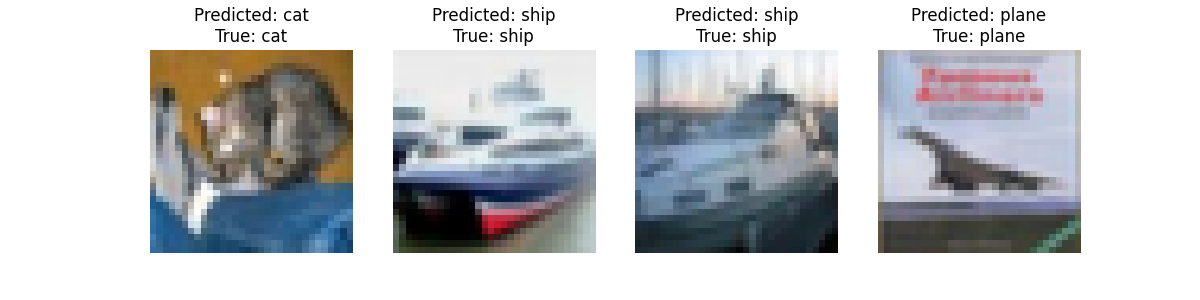
\includegraphics[width=1.0\textwidth]{train2.png}
    \caption{CNN Training Prediction}
    \label{fig:cnn_validation_accuracy}
\end{figure}

\begin{figure}[H]
    \centering
    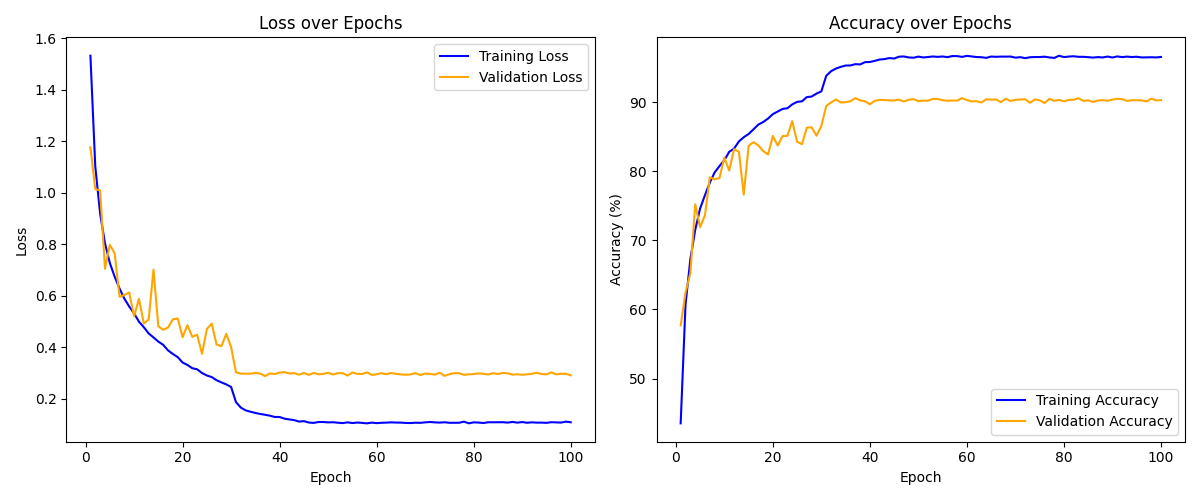
\includegraphics[width=1.0\textwidth]{train3.png}
    \caption{CNN's Loss and Accuracy on Training and Validation Sets}
    \label{fig:cnn_training_validation_loss_accuracy}
\end{figure}







\cleardoublepage



\section{CIFAR-10 上的卷积神经网络}

\subsection{CNN 概述}

卷积神经网络 (CNNs) 是专为处理网格状数据(如图像)而设计的专用架构,通过利用空间层次结构。其在图像识别中的有效性,特别是对于 CIFAR-10 等数据集,源于其能够在保持计算效率的同时提取局部特征 \cite{cifar10}。

\subsubsection{传统神经网络的局限性}

传统神经网络在处理图像数据时存在以下困难:

\begin{enumerate}[label=\roman*.]
    \item \textit{高输入维度}: 1000$\times$1000 像素的彩色图像需要 3,000,000 个输入神经元 (RGB 通道为 1000 $\times$ 1000 $\times$ 3),带来显著的计算挑战。
    \item \textit{参数过载}: 将其连接到具有 1000 个神经元的隐藏层需要 3,000,000,000 个权重,使训练和存储复杂化。
    \item \textit{空间上下文丢失}: 将图像展平为向量会丢弃对于识别边缘或纹理等模式至关重要的像素关系。
    \item \textit{缺乏平移不变性}: 图像中物体的偏移可能破坏识别,因为这些网络依赖于固定的像素模式。
\end{enumerate}

\subsubsection{CNN 的优势}

CNN 通过以下方式克服这些问题:

\begin{enumerate}[label=\roman*.]
    \item \textit{局部感受野}: 神经元连接到小的输入区域 (例如 3$\times$3 的块),减少参数。
    \item \textit{参数共享}: 具有固定权重的滤波器在图像上滑动,最小化参数并确保像边缘这样的特征被普遍检测到。
    \item \textit{空间下采样}: 池化层 (例如最大池化) 汇总区域,降低维度并增强对微小平移的鲁棒性。
\end{enumerate}

\subsection{CNN 架构}

典型的 CNN 堆叠卷积块以提取层次化特征,结构如下:

\begin{enumerate}[label=\roman*.]
    \item \textit{输入层}: 接收原始图像数据 (例如 CIFAR-10 为 32$\times$32$\times$3)。
    \item \textit{卷积层}: 应用滤波器通过以下公式生成特征图:
        \[
        S(i, j) = \sum_{m} \sum_{n} I(i + m, j + n) K(m, n),
        \]
        其中 $I$ 是输入,$K$ 是滤波器,$S$ 是特征图。
    \item \textit{激活层}: 使用 ReLU 引入非线性,$f(x) = \max(0, x)$,实现复杂模式学习 \cite{relu}。
    \item \textit{池化层}: 降低维度,例如最大池化选择 2$\times$2 区域中的最大值。
    \item \textit{堆叠块}: 早期层检测边缘,中间层捕获纹理,更深层识别物体。
    \item \textit{展平层}: 将特征图转换为向量。
    \item \textit{全连接层}: 组合特征进行分类。
    \item \textit{输出层}: 使用 Softmax 生成类别概率。
\end{enumerate}

\subsection{CIFAR-10 上的实现}

CIFAR-10 数据集包含 10 个类别的 50,000 张训练图像和 10,000 张测试图像,作为一个强大的测试平台 \cite{cifar10}。

\subsubsection{数据预处理}

为增强泛化能力:

\begin{itemize}
    \item \textit{增强}: 随机裁剪和水平翻转使训练数据多样化。
    \item \textit{标准化}: 使用 CIFAR-10 的均值和标准差对图像进行标准化。
    \item \textit{数据集划分}: 80\% 训练,20\% 验证,通过 \texttt{SubsetRandomSampler} 采样。
    \item \textit{批量大小}: 设置为 128 以实现高效训练。
\end{itemize}

\subsubsection{模型设计}

CNN 包含三个卷积块:

\begin{itemize}
    \item \textit{结构}: 每个块有两个 3$\times$3 卷积层、批量归一化 \cite{batchnorm}、ReLU 和最大池化。
    \item \textit{通道}: 从 64 增加到 128 再到 256,捕获复杂特征。
    \item \textit{空间缩减}: 图像尺寸从 32$\times$32 减小到 4$\times$4。
    \item \textit{输出}: 4$\times$4$\times$256 特征图展平为 4096 维,随后是具有 0.5 丢弃率 \cite{dropout} 的全连接层。
\end{itemize}

\begin{table}[h]
\centering
\caption{CNN 架构}
\begin{tabular}{l c c c}
\toprule
\textbf{层} & \textbf{输出形状} & \textbf{参数} & \textbf{操作} \\
\midrule
卷积块 1 & 32$\times$32$\times$64 & 3$\times$3 滤波器, BN, ReLU & 卷积 + 池化 \\
卷积块 2 & 16$\times$16$\times$128 & 3$\times$3 滤波器, BN, ReLU & 卷积 + 池化 \\
卷积块 3 & 8$\times$8$\times$256 & 3$\times$3 滤波器, BN, ReLU & 卷积 + 池化 \\
展平 & 4096 & -- & 重塑 \\
全连接 & 10 & 丢弃 (0.5) & 分类 \\
\bottomrule
\end{tabular}
\end{table}

\subsubsection{训练策略}

超过 100 个周期的训练使用了:

\begin{itemize}
    \item \textit{优化器}: 带动量的 SGD 以实现更快收敛。
    \item \textit{正则化}: 权重衰减 ($5 \times 10^{-4}$) 以抑制过拟合。
    \item \textit{调度器}: 如果验证损失在 5 个周期内停滞,则将学习率降低 10 倍。
\end{itemize}

\subsubsection{训练流程}

每个周期包括:

\begin{itemize}
    \item \textit{监控}: 每 100 个批次记录损失和准确率。
    \item \textit{验证}: 周期结束后评估性能以调整学习率。
    \item \textit{模型保存}: 基于验证准确率保留表现最佳的模型。
\end{itemize}

\subsubsection{评估}

该模型实现了 $\sim$90\% 的测试准确率,能够正确分类多样图像 (例如区分猫和狗)。

\subsection{性能分析}

到第 40 个周期,训练准确率超过 90\%,损失低于 10\%,而验证准确率达到 $\sim$90\%,损失约为 30\%。这些指标表明稳健的学习,尽管验证性能表明仍有改进空间。

% \begin{figure}[h]
% \centering
% \begin{subfigure}{0.45\textwidth}
%     \includegraphics[width=\textwidth]{training_loss.png}
%     \caption{训练和验证损失。}
% \end{subfigure}
% \hfill
% \begin{subfigure}{0.45\textwidth}
%     \includegraphics[width=\textwidth]{training_accuracy.png}
%     \caption{训练和验证准确率。}
% \end{subfigure}
% \caption{100 个周期内的性能曲线。}
% \end{figure}

% \begin{figure}[h]
% \centering
% \includegraphics[width=0.6\textwidth]{classification_examples.png}
% \caption{正确分类的 CIFAR-10 图像示例。}
% \end{figure}

\subsection{讨论}

90\% 的准确率反映了 CNN 的有效使用,并通过数据预处理和正则化得到增强。与达到 95\% 以上的 ResNet 等最先进模型相比 \cite{resnet},该模型表现稳健,但可能受益于更深层的架构或残差连接等先进技术。在第 40 个周期左右提前停止可以优化训练效率。

该实现强调了 CNN 在图像分类中的强大能力,并为进一步探索计算机视觉任务奠定了基础。

\cleardoublepage

\section{使用 ResNet 和 Vision Transformer 进行 CIFAR-10 图像分类}

\section*{引言}
% 介绍 CIFAR-10 数据集和目标
CIFAR-10 数据集包含 10 个类别 (例如飞机、汽车、鸟类) 的 60,000 张 32x32 彩色图像,是图像分类的基准数据集,其中包含 50,000 张训练图像和 10,000 张测试图像。本报告比较了两种神经网络模型——ResNet 和 Vision Transformer (ViT)——在 CIFAR-10 上的表现,评估了从头训练和微调预训练模型的效果。我们分析了性能、计算资源和实验结果,并提供了代码实现支持。

\section*{数据集和模型}
% 描述数据集和模型架构
\subsection*{CIFAR-10 数据集}
CIFAR-10 包含 10 个类别,每个类别 6,000 张图像,分为 50,000 张训练图像和 10,000 张测试图像,分布均匀。其低分辨率 (32x32) 测试了模型在小数据集上的性能。

\subsection*{ResNet}
残差网络 (ResNet) 使用跳跃连接来简化深度网络训练。评估了 ResNet-110 (170 万参数) 和 ResNet50 (2500 万参数)。

\subsection*{Vision Transformer (ViT)}
ViT 将图像分割成块并应用 Transformer 架构。ViT-B/16 (8600 万参数) 依赖大规模预训练以获得最佳性能。

\section*{数据划分和预处理}
% 详细说明数据预处理步骤
数据集分为 50,000 张训练图像和 10,000 张测试图像。预处理包括:
\begin{itemize}
    \item \textbf{训练}: 随机裁剪 (32x32,4 像素填充),随机水平翻转,标准化 (均值 [0.4914, 0.4822, 0.4465],标准差 [0.2023, 0.1994, 0.2010])。
    \item \textbf{测试}: 仅标准化。
\end{itemize}

\section*{从头训练}
% 比较从头训练的 ResNet 和 ViT
从头训练不使用预训练权重。ResNet 优于 ViT:
\begin{itemize}
    \item \textbf{ResNet-110}: 达到 93.57\% 准确率 (170 万参数),高效训练 \cite{he2016deep}。
    \item \textbf{ViT}: 标准 ViT 达到 77–88\% 准确率;优化版本达到 90.92\% (630 万参数) \cite{omihub777vitcifar, kentaroy47vit}。
\end{itemize}

\begin{table}[h]
\centering
\caption{从头训练的准确率和参数量}
\begin{tabular}{lccc}
\toprule
模型 & 准确率 (\%) & 参数量 (百万) & 备注 \\
\midrule
ResNet-110 & 93.57 & 1.7 & \cite{he2016deep} \\
ViT (标准) & 77–88 & 6.3 & 因配置而异 \cite{kentaroy47vit} \\
ViT (优化) & 90.92 & 6.3 & \cite{omihub777vitcifar} \\
\bottomrule
\end{tabular}
\end{table}

\section*{微调预训练模型}
% 比较在 CIFAR-10 上微调的预训练模型
预训练模型在大型数据集上训练后在 CIFAR-10 上微调:
\begin{itemize}
    \item \textbf{ResNet50 (ImageNet-1k)}: 92.34–92.63\% 准确率 \cite{sidthoviti}。
    \item \textbf{ViT base (ImageNet-1k)}: 98.5\% 准确率 \cite{kentaroy47vit}。
    \item \textbf{ViT-H/14 (JFT-300M)}: 99.50\% 准确率;ViT-L/16 (ImageNet-21k): 99.15\% \cite{dosovitskiy2020image}。
    \item \textbf{BiT-L (ResNet152x4, JFT-300M)}: 99.37\% \cite{dosovitskiy2020image}。
\end{itemize}

\begin{table}[h]
\centering
\caption{微调预训练模型的准确率}
\begin{tabular}{llcc}
\toprule
模型 & 预训练数据集 & 准确率 (\%) & 备注 \\
\midrule
ResNet50 & ImageNet-1k & 92.34–92.63 & \cite{sidthoviti} \\
ViT base & ImageNet-1k & 98.5 & \cite{kentaroy47vit} \\
ViT-H/14 & JFT-300M & 99.50 & \cite{dosovitskiy2020image} \\
ViT-L/16 & ImageNet-21k & 99.15 & \cite{dosovitskiy2020image} \\
BiT-L (ResNet152x4) & JFT-300M & 99.37 & \cite{dosovitskiy2020image} \\
\bottomrule
\end{tabular}
\end{table}

\section*{计算资源和性能}
% 分析计算成本
\begin{itemize}
    \item \textbf{ResNet}: 参数较少 (ResNet-110 为 170 万,ResNet50 为 2500 万),收敛快 (5 个周期内达到 90\% 准确率) \cite{pytorchforum}。
    \item \textbf{ViT}: 参数较多 (ViT-B/16 为 8600 万),初始学习较慢 (10,000 次迭代才稳定),但微调高效 \cite{lightningvit, dosovitskiy2020image}。
\end{itemize}

\section*{实验分析}
% 提供实验洞察
\subsection*{错误分析}
应分析错误分类的图像。ViT 可能在上下文丰富的类别 (例如猫与狗) 中表现出色,这归功于全局注意力,而 ResNet 在纹理细节 (例如飞机) 上表现更好 \cite{kentaroy47vit}。

\subsection*{性能差距原因}
CNN (ResNet) 利用归纳偏置 (例如平移不变性),适合小数据集。ViT 需要更多数据来学习模式 \cite{lightningvit}。

\subsection*{算法权衡}
\begin{itemize}
    \item \textbf{ResNet}: 高效,参数较少,适合小数据集;在大数据集上可扩展性较差。
    \item \textbf{ViT}: 在大规模预训练下表现优异,灵活,但资源密集且容易在小数据集上过拟合。
\end{itemize}

\section*{可视化}
% Presenting visualization code
准确率可以通过条形图进行可视化。以下是一个用于比较的 Python 代码片段:

\begin{lstlisting}[language=Python]
import matplotlib.pyplot as plt
models = ['ResNet-110', 'ViT (Standard)', 'ViT (Optimized)']
accuracies = [93.57, 88, 90.92]
plt.bar(models, accuracies, color=['#1f77b4', '#ff7f0e', '#2ca02c'])
plt.xlabel('Model')
plt.ylabel('Accuracy (\%)')
plt.title('CIFAR-10 Accuracy (Training from Scratch)')
plt.show()
\end{lstlisting}

\section*{定量指标}
% 总结关键指标
\begin{itemize}
    \item \textbf{准确率}: 参见表1和表2。
    \item \textbf{参数量}: ResNet-110 (1.7M), ResNet50 (25M), ViT-B/16 (86M), ViT (优化版, 6.3M).
    \item \textbf{训练时间}: ResNet-110 可在数小时内达到 90\%+ 准确率; ViT 需要更长时间 (10000 次迭代)。
    \item \textbf{资源需求}: ViT 预训练需要高端 GPU (例如 V100); ResNet 可在标准 GPU 上高效训练。
\end{itemize}

\section*{代码实现}
% Providing training code for ResNet and ViT
\subsection*{ResNet Training}
\begin{lstlisting}[language=Python]
import torch
import torch.nn as nn
import torchvision
import torchvision.transforms as transforms
import torch.optim as optim

device = torch.device('cuda' if torch.cuda.is_available() else 'cpu')

transform_train = transforms.Compose([
    transforms.RandomCrop(32, padding=4),
    transforms.RandomHorizontalFlip(),
    transforms.ToTensor(),
    transforms.Normalize((0.4914, 0.4822, 0.4465), (0.2023, 0.1994, 0.2010))
])
transform_test = transforms.Compose([
    transforms.ToTensor(),
    transforms.Normalize((0.4914, 0.4822, 0.4465), (0.2023, 0.1994, 0.2010))
])

train_dataset = torchvision.datasets.CIFAR10(root='./data', train=True, download=True, transform=transform_train)
test_dataset = torchvision.datasets.CIFAR10(root='./data', train=False, download=True, transform=transform_test)
train_loader = torch.utils.data.DataLoader(train_dataset, batch_size=128, shuffle=True)
test_loader = torch.utils.data.DataLoader(test_dataset, batch_size=128, shuffle=False)

model = torchvision.models.resnet18(pretrained=False, num_classes=10)
model.conv1 = nn.Conv2d(3, 64, kernel_size=3, stride=1, padding=1, bias=False)
model.maxpool = nn.Identity()
model = model.to(device)

criterion = nn.CrossEntropyLoss()
optimizer = optim.SGD(model.parameters(), lr=0.1, momentum=0.9, weight_decay=1e-4)

num_epochs = 50
for epoch in range(num_epochs):
    model.train()
    running_loss = 0.0
    for i, (images, labels) in enumerate(train_loader):
        images, labels = images.to(device), labels.to(device)
        optimizer.zero_grad()
        outputs = model(images)
        loss = criterion(outputs, labels)
        loss.backward()
        optimizer.step()
        running_loss += loss.item()
    print(f'Epoch [{epoch+1}/{num_epochs}], Loss: {running_loss/len(train_loader):.4f}')

model.eval()
correct = 0
total = 0
with torch.no_grad():
    for images, labels in test_loader:
        images, labels = images.to(device), labels.to(device)
        outputs = model(images)
        _, predicted = torch.max(outputs.data, 1)
        total += labels.size(0)
        correct += (predicted == labels).sum().item()
print(f'Test Accuracy: {100 * correct / total}\%')
\end{lstlisting}

\begin{figure}[H]
    \centering
    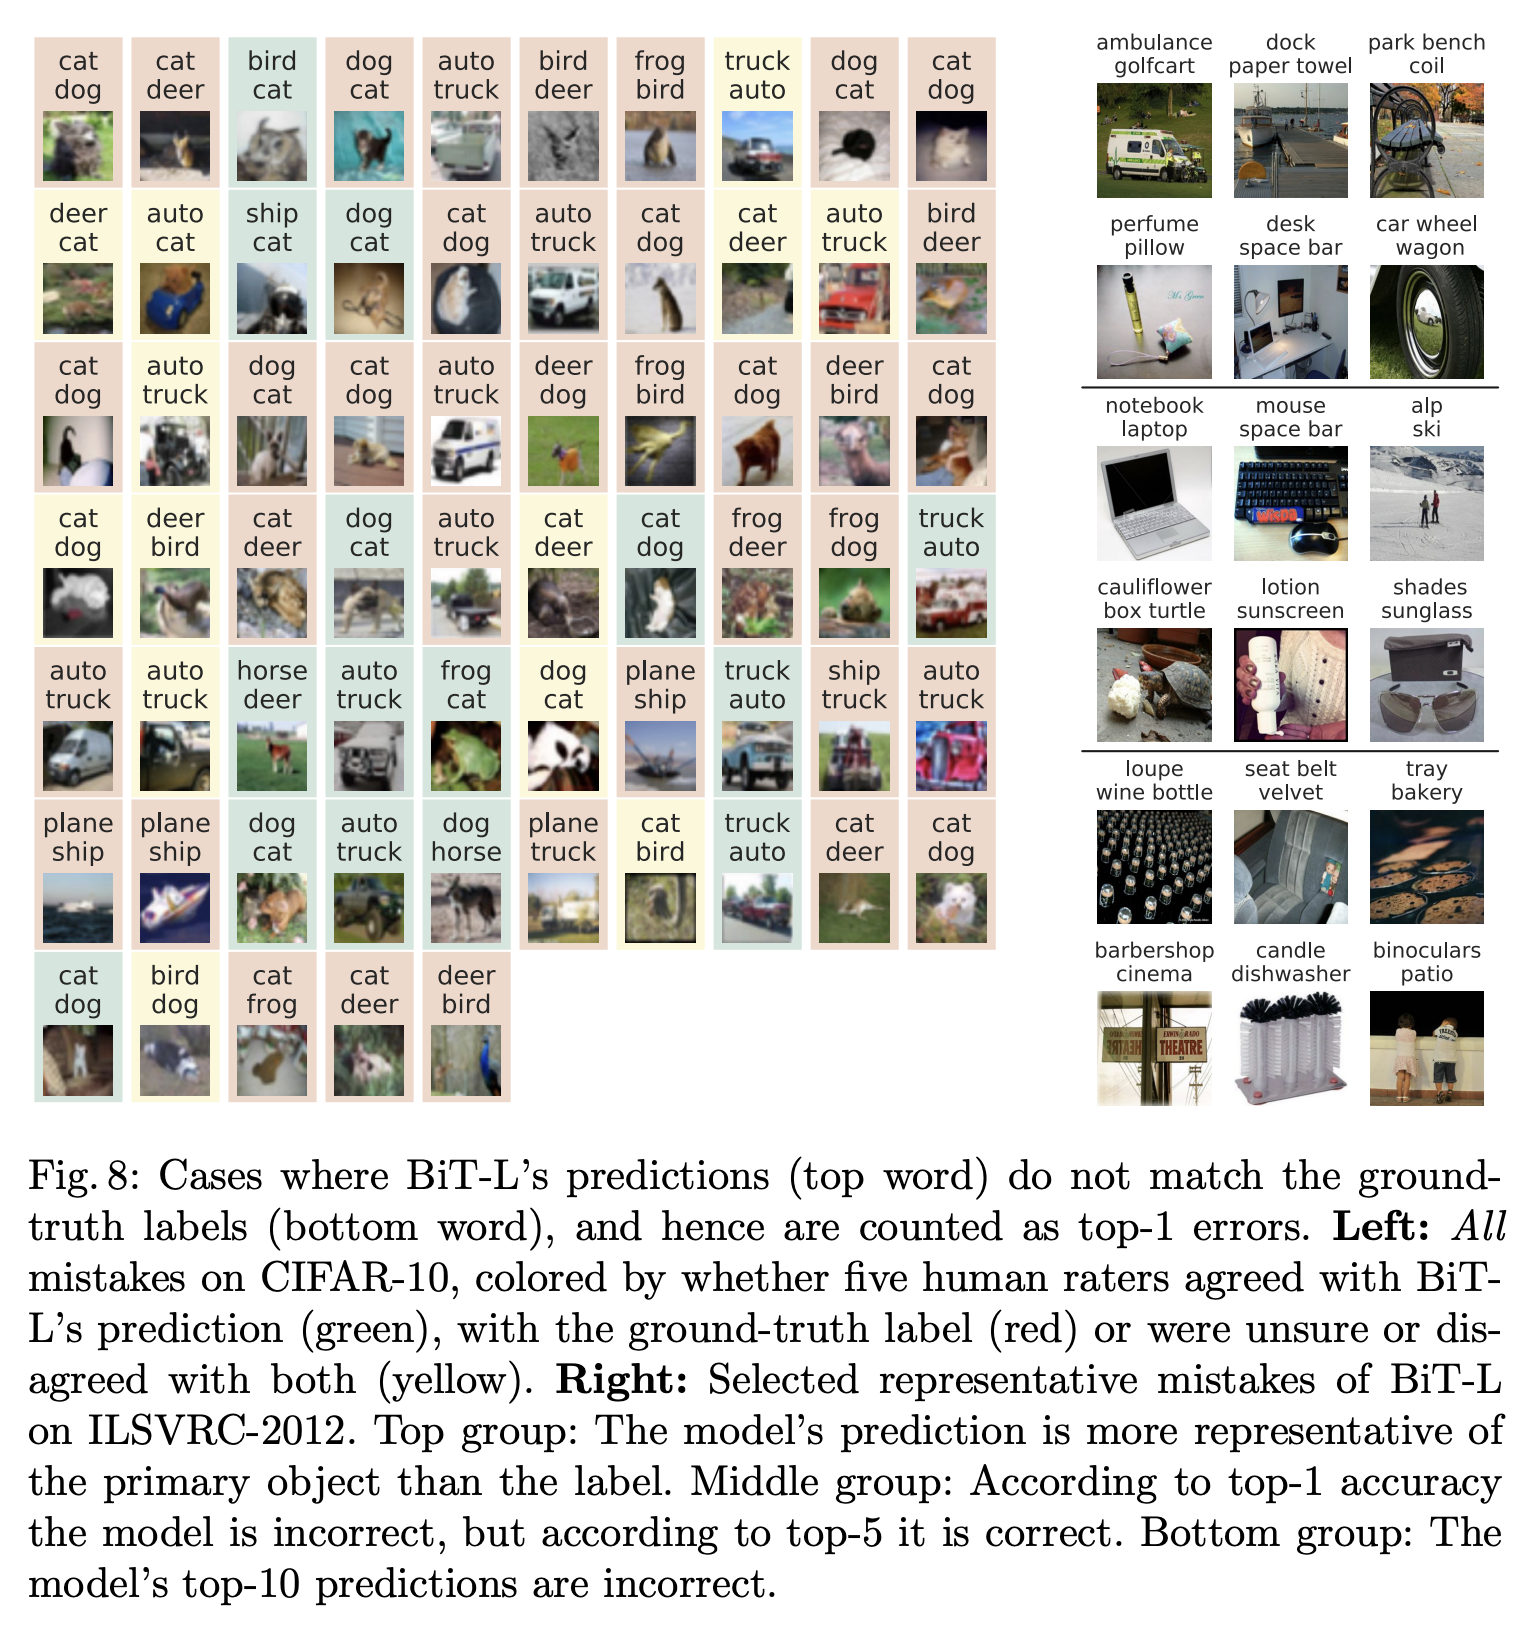
\includegraphics[width=1.0\textwidth]{ResNet.png}
    \caption{ResNet Architecture}
    \label{fig:resnet_architecture}
\end{figure}

\subsection*{ViT Fine-Tuning}
\begin{lstlisting}[language=Python]
import torch
from transformers import ViTForImageClassification, ViTFeatureExtractor
from torchvision import datasets, transforms
from torch.utils.data import DataLoader

device = torch.device('cuda' if torch.cuda.is_available() else 'cpu')

transform = transforms.Compose([
    transforms.Resize((224, 224)),
    transforms.ToTensor(),
    transforms.Normalize(mean=[0.5, 0.5, 0.5], std=[0.5, 0.5, 0.5])
])

train_dataset = datasets.CIFAR10(root='./data', train=True, download=True, transform=transform)
test_dataset = datasets.CIFAR10(root='./data', train=False, download=True, transform=transform)
train_loader = DataLoader(train_dataset, batch_size=32, shuffle=True)
test_loader = DataLoader(test_dataset, batch_size=32, shuffle=False)

model = ViTForImageClassification.from_pretrained('google/vit-base-patch16-224-in21k', num_labels=10)
model = model.to(device)

optimizer = torch.optim.Adam(model.parameters(), lr=2e-5)
criterion = torch.nn.CrossEntropyLoss()

num_epochs = 5
for epoch in range(num_epochs):
    model.train()
    running_loss = 0.0
    for images, labels in train_loader:
        images, labels = images.to(device), labels.to(device)
        optimizer.zero_grad()
        outputs = model(images).logits
        loss = criterion(outputs, labels)
        loss.backward()
        optimizer.step()
        running_loss += loss.item()
    print(f'Epoch [{epoch+1}/{num_epochs}], Loss: {running_loss/len(train_loader):.4f}')

model.eval()
correct = 0
total = 0
with torch.no_grad():
    for images, labels in test_loader:
        images, labels = images.to(device), labels.to(device)
        outputs = model(images).logits
        _, predicted = torch.max(outputs.data, 1)
        total += labels.size(0)
        correct += (predicted == labels).sum().item()
print(f'Test Accuracy: {100 * correct / total}\%')
\end{lstlisting}

\begin{figure}[H]
    \centering
    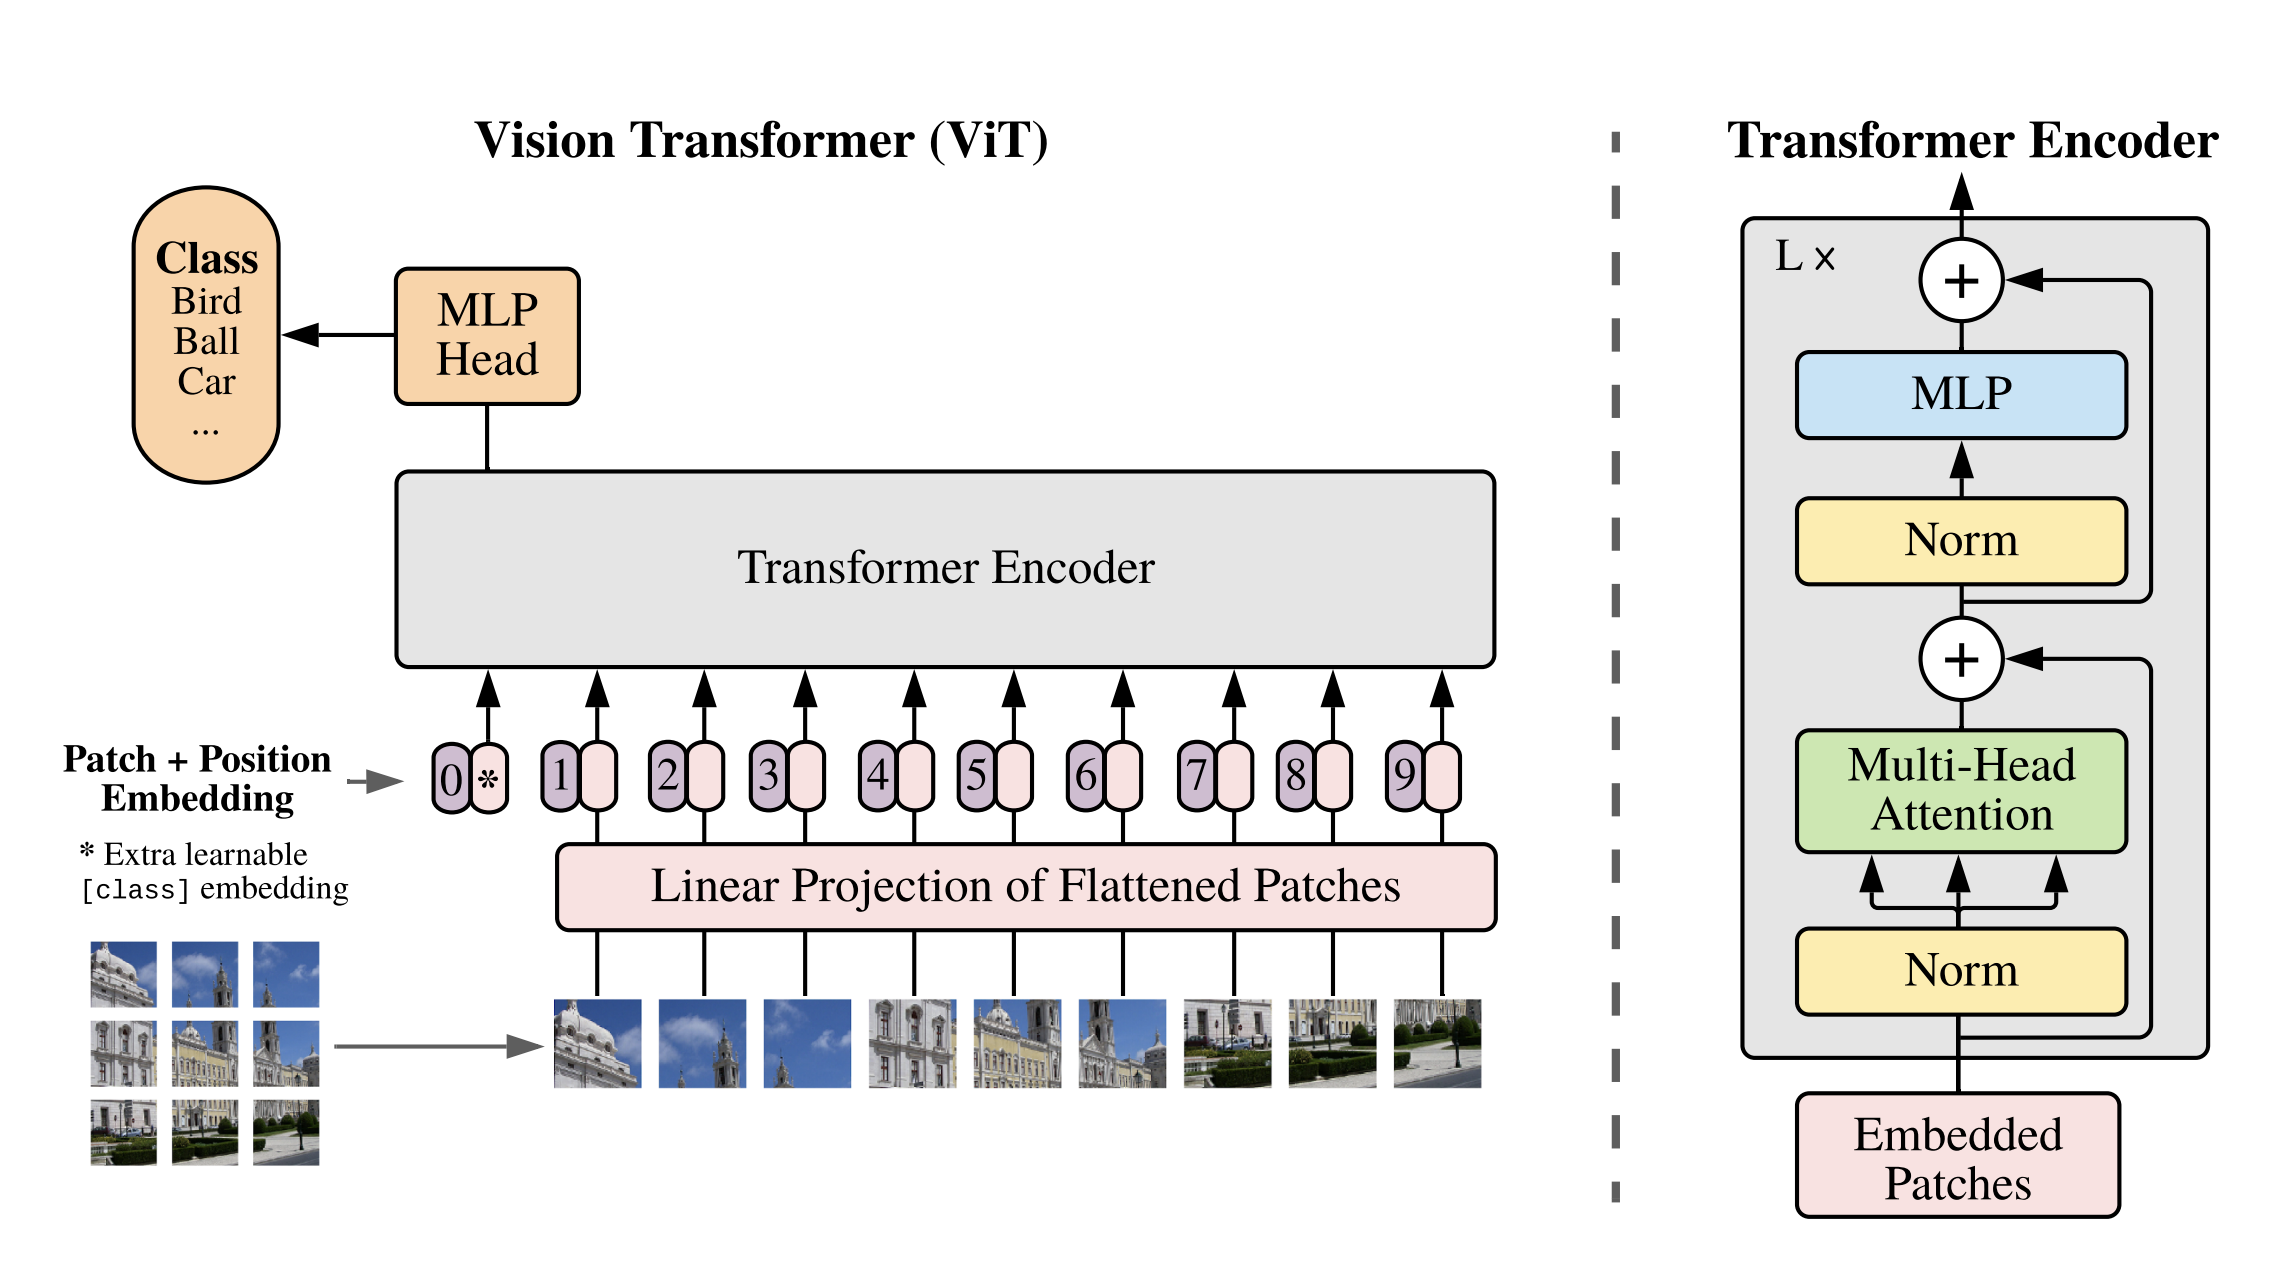
\includegraphics[width=1.0\textwidth]{ViT1.png}
    \caption{ViT Transformer}
    \label{fig:vit_transformer}
\end{figure}

\begin{figure}[H]
    \centering
    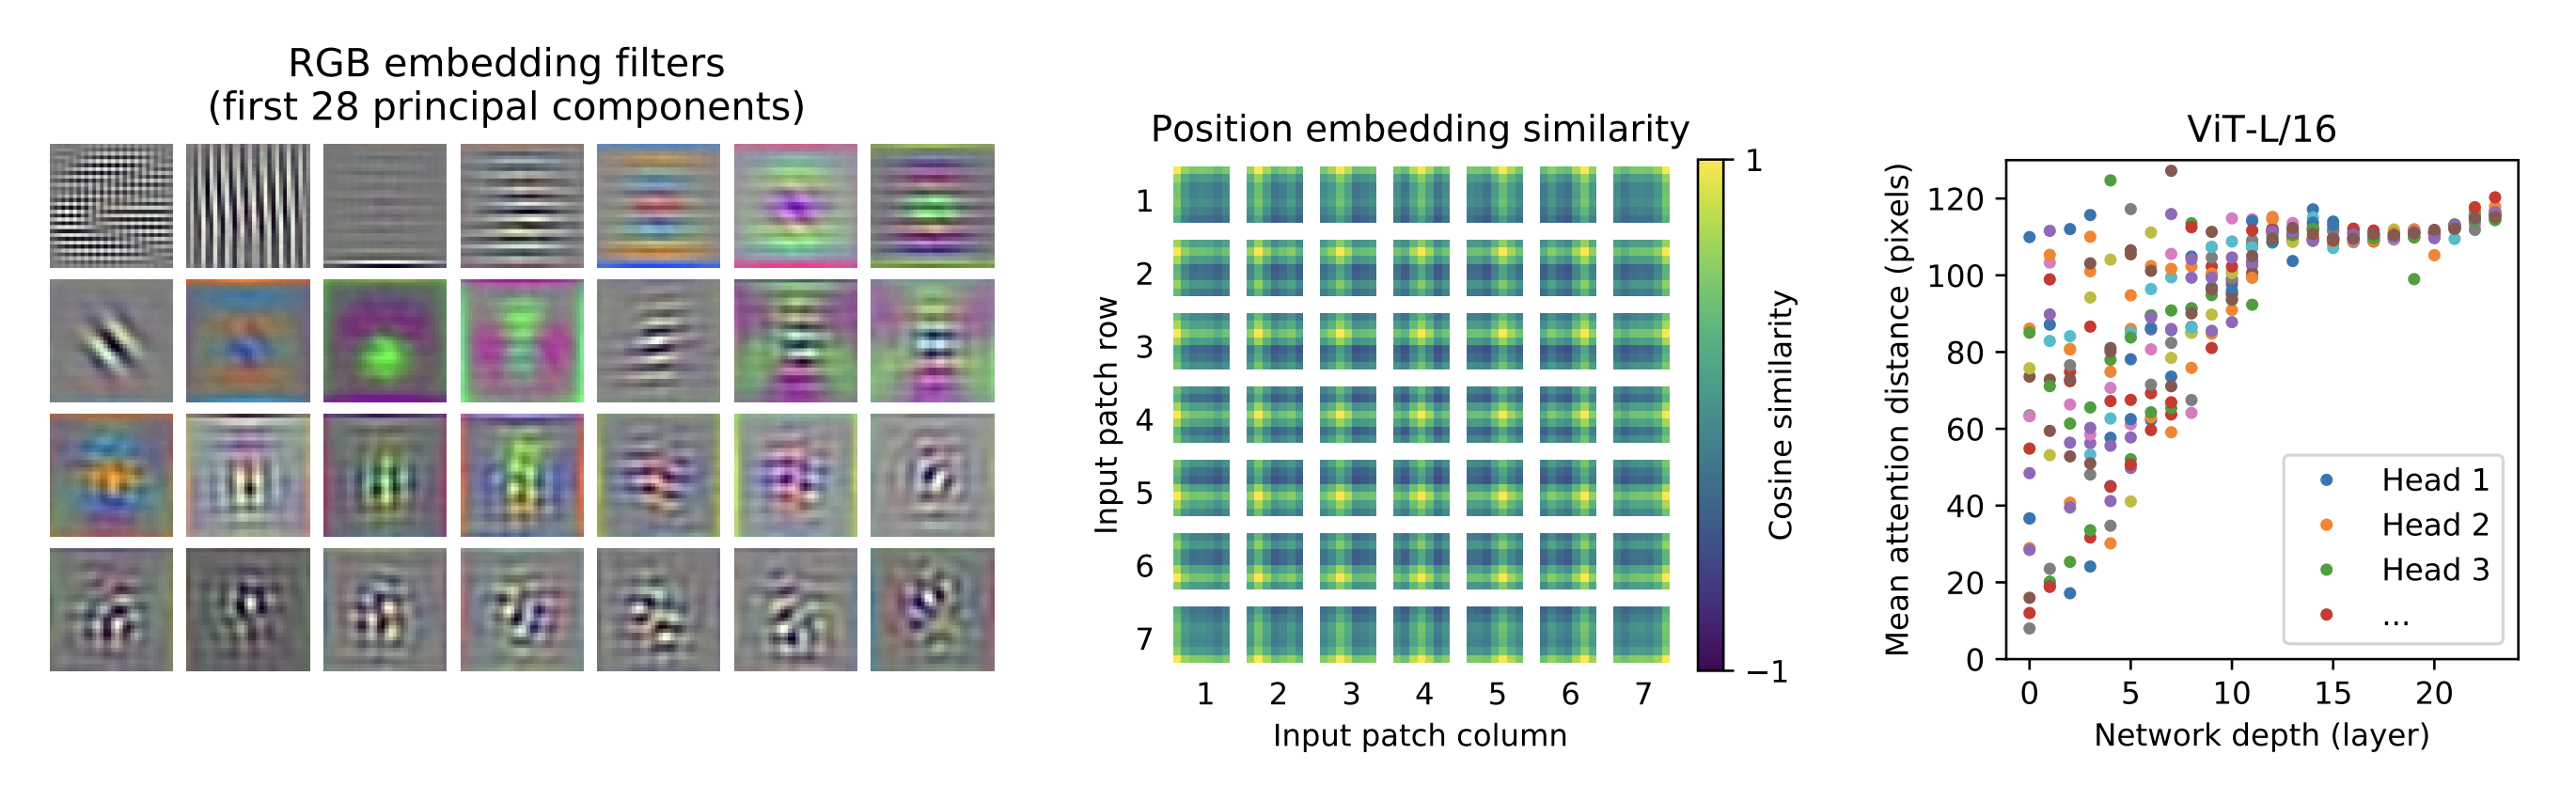
\includegraphics[width=1.0\textwidth]{ViT2.png}
    \caption{ViT Training}
    \label{fig:vit_training}
\end{figure}


\section*{结论}
% Summarizing findings
ResNet-110 在 CIFAR-10 上从头开始训练表现出色(93.57\% 准确率,低计算成本)。预训练的 ViT 模型,特别是从 JFT-300M 微调而来的 ViT-H/14(99.50\%),性能优于 ResNet(BiT-L,99.37\%)。模型选择取决于数据规模和资源:ResNet 适合数据/资源有限的情况,而 ViT 在大规模预训练下表现优异。提供代码实现以确保可复现性。




\chapter{非线性方法分类器}
\section{非线性方法分类器简介}
在本节中我们着重介绍核化支持向量机(Kernel SVM)、决策树(Decision Tree)两种代表性的非线性分类模型,以及基于决策树衍生而来的随机森林(Random Forest)分类器,并基于选定的数据集进行实验和对比分析。

\subsection{Kernel SVM}
在传统线性SVM的基础上,通过在低维空间中引入核函数,将原始特征映射到更高维度的特征空间,从而使得线性分类器能够捕捉更复杂的非线性关系。常用的核函数包括多项式核和径向基核函数(RBF)等。通过恰当选择或组合核函数,Kernel SVM在复杂的数据集上往往能取得较为良好的分类性能。

\subsection{决策树(Decision Tree)}
决策树通过一系列特征选择步骤对数据进行逐层划分,实现对类别的划分。其优点在于易于理解与可视化,但单棵决策树在训练过程中可能会出现过拟合、对噪声敏感等问题。常见的决策树划分准则包括信息增益和基尼指数等。
\section{随机森林(Random Forest)简介}
虽然随机森林方法并不属于非线性方法分类器,但是由于其与决策树的相关性,我们决定将其置于该章节与决策树方法进行对比。随机森林是一种基于Bagging思想的集成学习方法,通过训练多棵独立的决策树并对其结果进行投票或平均来完成分类。不同决策树的训练通常使用带放回的随机采样(Bootstrap)与随机特征选择,以降低模型的方差并减少过拟合风险。随机森林相较于单棵决策树通常在精度、稳定性等方面都有显著提升。

\section{实验选择分类器详解}

\subsection{决策树详细介绍}

决策树(Decision Tree)是一种重要的非线性分类算法,通过构建树状结构模型来实现对数据的分类和预测。其直观的结构和良好的可解释性使其在机器学习领域广泛应用。

\subsubsection{决策树的定义与基本原理}

决策树是一种基于树状结构的监督学习算法,通过一系列if-then规则将样本从根节点逐步分配到叶节点,最终完成分类任务。决策树的核心思想是寻找最优的特征和分割点,使得每次分割后的子集在类别上更加纯净。

根据Scikit-learn Documentation的《Decision Trees》,决策树的学习过程本质上是一个递归的特征选择和样本分割过程,通过最大化信息增益或最小化基尼不纯度来选择最优分割。

\subsubsection{决策树的关键组成}

决策树主要包含以下关键组成部分:

\begin{itemize}
    \item \textbf{根节点(Root Node)}:包含所有训练样本的起始节点
    \item \textbf{内部节点(Internal Node)}:表示一个特征上的测试条件
    \item \textbf{叶节点(Leaf Node)}:表示类别标签或预测结果
    \item \textbf{分支(Branch)}:连接节点,表示测试结果
\end{itemize}

\subsubsection{分割准则与算法原理}

决策树构建的核心是选择最优的分割特征和分割点。常用的分割准则包括:

\paragraph{信息增益(Information Gain)}
基于信息论中的熵概念,信息增益定义为:
\begin{equation}
\text{Gain}(S, A) = \text{Entropy}(S) - \sum_{v \in \text{Values}(A)} \frac{|S_v|}{|S|} \text{Entropy}(S_v)
\end{equation}
其中,熵的计算公式为:
\begin{equation}
\text{Entropy}(S) = -\sum_{i=1}^{c} p_i \log_2 p_i
\end{equation}

\paragraph{基尼不纯度(Gini Impurity)}
基尼不纯度衡量样本集合的不纯程度:
\begin{equation}
\text{Gini}(S) = 1 - \sum_{i=1}^{c} p_i^2
\end{equation}
基尼增益定义为:
\begin{equation}
\text{Gini\_Gain}(S, A) = \text{Gini}(S) - \sum_{v \in \text{Values}(A)} \frac{|S_v|}{|S|} \text{Gini}(S_v)
\end{equation}

\paragraph{信息增益率(Gain Ratio)}
为避免信息增益偏向取值较多的特征,引入信息增益率:
\begin{equation}
\text{Gain\_Ratio}(S, A) = \frac{\text{Gain}(S, A)}{\text{Split\_Info}(S, A)}
\end{equation}
其中分割信息定义为:
\begin{equation}
\text{Split\_Info}(S, A) = -\sum_{v \in \text{Values}(A)} \frac{|S_v|}{|S|} \log_2 \frac{|S_v|}{|S|}
\end{equation}

\begin{table}[h]
\centering
\caption{决策树分割准则对比}
\begin{tabular}{l p{3cm} p{4cm} p{3cm}}
\toprule
\textbf{分割准则} & \textbf{计算复杂度} & \textbf{优点} & \textbf{缺点} \\
\midrule
信息增益 & 中等 & 理论基础扎实,易于理解 & 偏向取值多的特征 \\
基尼不纯度 & 较低 & 计算简单,收敛快 & 对类别不平衡敏感 \\
信息增益率 & 较高 & 避免偏向性,更公平 & 计算复杂度高 \\
\bottomrule
\end{tabular}
\end{table}

\subsubsection{决策树算法流程}

经典的决策树构建算法(如ID3、C4.5、CART)遵循以下基本流程:

\begin{enumerate}[label=\arabic*.]
    \item \textbf{初始化}:将所有训练样本放在根节点
    \item \textbf{特征选择}:计算所有特征的分割准则值,选择最优特征
    \item \textbf{节点分割}:根据最优特征将样本分割到子节点
    \item \textbf{递归构建}:对每个子节点重复步骤2-3
    \item \textbf{停止条件}:满足以下条件之一则停止:
        \begin{itemize}
            \item 节点中所有样本属于同一类别
            \item 没有可用特征进行分割
            \item 达到预设的最大深度
            \item 节点样本数量少于最小分割阈值
        \end{itemize}
\end{enumerate}

\subsubsection{决策树算法比较}

\begin{table}[h]
\centering
\caption{主要决策树算法对比}
\begin{tabular}{l p{2.5cm} p{3cm} p{3cm} p{3cm}}
\toprule
\textbf{算法} & \textbf{分割准则} & \textbf{处理连续特征} & \textbf{处理缺失值} & \textbf{剪枝策略} \\
\midrule
ID3 & 信息增益 & 不支持 & 不支持 & 无 \\
C4.5 & 信息增益率 & 支持(二分法) & 支持 & 后剪枝 \\
CART & 基尼不纯度 & 支持(二分法) & 代理分割 & 预剪枝+后剪枝 \\
\bottomrule
\end{tabular}
\end{table}

\subsubsection{过拟合问题与剪枝技术}

决策树容易出现过拟合,特别是在深度较大时。剪枝技术是解决过拟合的主要方法:

\paragraph{预剪枝(Pre-pruning)}
在树构建过程中提前停止,常用条件包括:
\begin{itemize}
    \item 最大深度限制
    \item 最小样本分割数
    \item 最小叶节点样本数
    \item 信息增益阈值
\end{itemize}

\paragraph{后剪枝(Post-pruning)}
先构建完整树,再通过验证集进行剪枝。CART算法采用成本复杂度剪枝:
\begin{equation}
C_\alpha(T) = C(T) + \alpha |T|
\end{equation}
其中$C(T)$是树的误分类代价,$|T|$是叶节点数,$\alpha$是复杂度参数。

\subsubsection{决策树的优势与局限}

\paragraph{优势}
\begin{itemize}
    \item \textbf{可解释性强}:树结构直观,规则明确
    \item \textbf{无需数据预处理}:不需要特征缩放或标准化
    \item \textbf{处理混合数据}:同时处理数值型和类别型特征
    \item \textbf{计算效率高}:训练和预测时间复杂度相对较低
    \item \textbf{特征选择}:能够识别重要特征
\end{itemize}

\paragraph{局限性}
\begin{itemize}
    \item \textbf{容易过拟合}:特别是对于高维数据
    \item \textbf{不稳定性}:数据的小变化可能导致树结构大变
    \item \textbf{偏向性}:倾向于选择取值较多的特征
    \item \textbf{难处理线性关系}:对于线性可分数据效果不佳
    \item \textbf{缺乏平滑性}:预测结果是阶跃函数
\end{itemize}





\subsection{随机森林详细介绍}

随机森林(Random Forest)是一种基于集成学习思想的强大非线性分类算法,通过构建多个决策树并结合其预测结果来提高模型的准确性和稳定性。作为决策树的重要扩展,随机森林有效解决了单一决策树容易过拟合和不稳定的问题。

\subsubsection{随机森林与决策树的关系}

随机森林本质上是决策树的集成版本,它们之间存在密切的继承和发展关系:

\begin{itemize}
    \item \textbf{基础构建块}:随机森林以决策树为基本学习器,每棵树都是一个完整的决策树分类器
    \item \textbf{问题解决}:针对单一决策树的高方差和过拟合问题,随机森林通过集成多棵树来降低方差
    \item \textbf{预测机制}:单一决策树给出确定性预测,而随机森林通过多数投票(分类)或平均(回归)来做最终决策
    \item \textbf{特征处理}:决策树在每个节点考虑所有特征,随机森林在每个节点只考虑特征的随机子集
\end{itemize}

随机森林通过引入两层随机性(样本随机和特征随机)来构建多样化的决策树集合。

\subsubsection{随机森林的核心原理}

随机森林基于以下核心思想构建:

\paragraph{Bagging(Bootstrap Aggregating)}
随机森林采用Bootstrap采样方法从原始训练集中有放回地抽取多个子数据集:
\begin{equation}
D_i = \text{Bootstrap}(D, n), \quad i = 1, 2, \ldots, T
\end{equation}
其中$D$是原始数据集,$n$是采样大小(通常等于原数据集大小),$T$是树的数量。

\paragraph{特征随机选择}
在每个决策树的每个内部节点分裂时,从$d$个特征中随机选择$m$个特征子集:
\begin{equation}
m = \sqrt{d} \quad \text{(分类任务)}
\end{equation}
\begin{equation}
m = \frac{d}{3} \quad \text{(回归任务)}
\end{equation}

\paragraph{集成预测}
对于分类任务,随机森林的最终预测通过多数投票机制:
\begin{equation}
\hat{y} = \text{mode}\{h_1(\mathbf{x}), h_2(\mathbf{x}), \ldots, h_T(\mathbf{x})\}
\end{equation}
其中$h_i(\mathbf{x})$表示第$i$棵树对样本$\mathbf{x}$的预测。

\subsubsection{随机森林算法流程}

随机森林的训练过程可以概括为以下步骤:

\begin{enumerate}[label=\arabic*.]
    \item \textbf{参数设置}:确定树的数量$T$、特征子集大小$m$、树的最大深度等
    \item \textbf{Bootstrap采样}:对每棵树$i$,从训练集$D$中有放回采样得到$D_i$
    \item \textbf{决策树构建}:对每棵树:
        \begin{itemize}
            \item 在每个节点分裂时随机选择$m$个特征
            \item 在这$m$个特征中选择最优分裂特征和分裂点
            \item 递归构建直到满足停止条件
        \end{itemize}
    \item \textbf{模型集成}:保存所有训练好的决策树
    \item \textbf{预测阶段}:对新样本,所有树进行预测并通过投票得到最终结果
\end{enumerate}

\begin{table}[h]
\centering
\caption{随机森林与单一决策树对比}
\begin{tabular}{l p{4cm} p{4cm}}
\toprule
\textbf{比较维度} & \textbf{单一决策树} & \textbf{随机森林} \\
\midrule
模型复杂度 & 单一树结构,复杂度较低 & 多树集成,复杂度较高 \\
过拟合风险 & 容易过拟合,特别是深树 & 通过集成显著降低过拟合 \\
方差水平 & 高方差,对数据变化敏感 & 低方差,预测更稳定 \\
偏差水平 & 偏差取决于树的深度 & 偏差与单树相近 \\
训练时间 & 快速训练 & 较长(可并行化) \\
预测时间 & 快速预测 & 相对较慢(需要多树预测) \\
可解释性 & 高度可解释 & 可解释性降低 \\
特征重要性 & 基于单树的特征使用 & 更robust的特征重要性 \\
\bottomrule
\end{tabular}
\end{table}

\subsubsection{随机森林的关键优势}

\paragraph{降低过拟合}
通过集成多个在不同数据子集上训练的决策树,随机森林有效降低了单一决策树的过拟合风险。根据统计学习理论,集成方法的泛化误差可以分解为:
\begin{equation}
\text{Error} = \text{Bias}^2 + \text{Variance} + \text{Noise}
\end{equation}
随机森林主要通过降低方差项来提高性能。

\paragraph{处理缺失值}
随机森林能够自然处理缺失值,通过以下方式:
\begin{itemize}
    \item 训练时:使用代理分裂(surrogate splits)
    \item 预测时:计算相似度权重进行填补
\end{itemize}

\paragraph{特征重要性评估}
随机森林提供两种特征重要性度量:
\begin{itemize}
    \item \textbf{平均不纯度减少}:计算每个特征在所有树中导致的不纯度减少的平均值
    \item \textbf{置换重要性}:通过随机打乱特征值观察性能下降程度
\end{itemize}

\subsubsection{超参数调优}

随机森林的关键超参数及其影响:

\begin{table}[h]
\centering
\caption{随机森林关键超参数}
\begin{tabular}{l p{3cm} p{4cm} p{3.5cm}}
\toprule
\textbf{参数} & \textbf{典型取值} & \textbf{影响} & \textbf{调优建议} \\
\midrule
n\_estimators & 100-1000 & 树的数量,影响性能和计算时间 & 先粗调再细调,观察收敛点 \\
max\_features & $\sqrt{d}$, $\log_2(d)$, $d/3$ & 每次分裂考虑的特征数 & 分类任务推荐$\sqrt{d}$ \\
max\_depth & 10-50或None & 树的最大深度 & 根据数据复杂度调整 \\
min\_samples\_split & 2-20 & 内部节点分裂所需最小样本数 & 防止过拟合的重要参数 \\
min\_samples\_leaf & 1-10 & 叶节点最小样本数 & 与min\_samples\_split协调 \\
bootstrap & True/False & 是否使用Bootstrap采样 & 通常保持True \\
\bottomrule
\end{tabular}
\end{table}

\subsubsection{理论基础与收敛性}

\paragraph{Bagging的理论基础}
对于回归问题,假设有$T$个独立的模型$f_1, f_2, \ldots, f_T$,每个模型的误差为$\epsilon_i$,则Bagging后的误差为:
\begin{equation}
\text{MSE}_{\text{ensemble}} = \frac{1}{T^2} \sum_{i=1}^{T} \text{MSE}_i + \frac{2}{T^2} \sum_{i<j} \text{Cov}(\epsilon_i, \epsilon_j)
\end{equation}

当模型间相关性降低时,集成效果显著提升。

\paragraph{袋外估计(Out-of-Bag, OOB)}
由于Bootstrap采样的特性,约有36.8\%的样本不会被选中(袋外样本):
\begin{equation}
P(\text{样本不被选中}) = \left(1 - \frac{1}{n}\right)^n \approx \frac{1}{e} \approx 0.368
\end{equation}

OOB样本可用于模型验证,无需额外的验证集。



\subsubsection{局限性与改进方向}

\paragraph{随机森林的局限性}
\begin{itemize}
    \item \textbf{高维稀疏数据}:在特征数远大于样本数时性能下降
    \item \textbf{线性关系}:对于线性可分数据,性能不如线性模型
    \item \textbf{内存消耗}:需要存储多棵完整的决策树
    \item \textbf{图像数据}:对于图像等结构化数据,不如深度学习方法
\end{itemize}

\paragraph{改进方向}
\begin{itemize}
    \item \textbf{Extra Trees}:在选择分裂点时引入更多随机性
    \item \textbf{特征工程}:结合深度学习提取的特征
    \item \textbf{混合模型}:与其他算法组合使用
    \item \textbf{在线学习}:支持增量学习的变种
\end{itemize}


\subsection{核支持向量机详细介绍}

核支持向量机(Kernel Support Vector Machine, Kernel SVM)是支持向量机(SVM)的重要扩展,通过引入核函数将线性SVM扩展到非线性分类问题。作为一种强大的非线性分类器,核SVM在处理复杂数据模式方面展现出卓越的性能。

\subsubsection{从线性SVM到核SVM的演进}

\paragraph{线性SVM的局限性}
线性支持向量机通过寻找最优分离超平面来解决分类问题,其目标是最大化分类间隔:
\begin{equation}
\min_{w,b} \frac{1}{2}\|w\|^2 + C\sum_{i=1}^{n}\xi_i
\end{equation}
其中$w$为权重向量,$b$为偏置项,$\xi_i$为松弛变量,$C$为正则化参数。

然而,线性SVM只能处理线性可分或近似线性可分的数据,对于复杂的非线性分布数据效果有限。

\paragraph{核技巧的引入}
为解决非线性分类问题,核SVM引入了核技巧(Kernel Trick),其核心思想是:
\begin{itemize}
    \item 通过非线性映射$\phi(\mathbf{x})$将原始特征空间映射到高维特征空间
    \item 在高维空间中应用线性SVM
    \item 利用核函数$K(\mathbf{x}_i, \mathbf{x}_j) = \phi(\mathbf{x}_i) \cdot \phi(\mathbf{x}_j)$避免显式计算高维映射
\end{itemize}

\subsubsection{核函数理论基础}

\paragraph{核函数的定义}
核函数是一个满足Mercer条件的函数$K: \mathcal{X} \times \mathcal{X} \rightarrow \mathbb{R}$,使得存在特征空间$\mathcal{H}$和映射$\phi: \mathcal{X} \rightarrow \mathcal{H}$,满足:
\begin{equation}
K(\mathbf{x}_i, \mathbf{x}_j) = \langle\phi(\mathbf{x}_i), \phi(\mathbf{x}_j)\rangle_{\mathcal{H}}
\end{equation}

\paragraph{Mercer条件}
一个函数$K(\mathbf{x}, \mathbf{z})$是有效核函数当且仅当对任意有限集$\{\mathbf{x}_1, \mathbf{x}_2, \ldots, \mathbf{x}_n\}$,核矩阵$\mathbf{K}$是半正定的:
\begin{equation}
K_{ij} = K(\mathbf{x}_i, \mathbf{x}_j), \quad \mathbf{K} \succeq 0
\end{equation}

\subsubsection{常用核函数类型}

\paragraph{线性核(Linear Kernel)}
最简单的核函数,实质上等同于原始线性SVM:
\begin{equation}
K(\mathbf{x}_i, \mathbf{x}_j) = \mathbf{x}_i^T \mathbf{x}_j
\end{equation}
适用于高维稀疏数据或线性可分问题。

\paragraph{径向基函数核(RBF Kernel)}
也称为高斯核,是最常用的非线性核函数:
\begin{equation}
K(\mathbf{x}_i, \mathbf{x}_j) = \exp\left(-\gamma \|\mathbf{x}_i - \mathbf{x}_j\|^2\right)
\end{equation}
其中$\gamma > 0$控制核的宽度。RBF核将数据映射到无限维空间,理论上可以处理任意复杂的非线性关系。

\paragraph{多项式核(Polynomial Kernel)}
通过多项式函数构建非线性映射:
\begin{equation}
K(\mathbf{x}_i, \mathbf{x}_j) = (\gamma \mathbf{x}_i^T \mathbf{x}_j + r)^d
\end{equation}
其中$d$为多项式阶数,$\gamma > 0$为尺度参数,$r \geq 0$为偏移参数。

\paragraph{Sigmoid核}
基于双曲正切函数的核函数:
\begin{equation}
K(\mathbf{x}_i, \mathbf{x}_j) = \tanh(\gamma \mathbf{x}_i^T \mathbf{x}_j + r)
\end{equation}
在特定参数下可近似神经网络的激活函数。

\begin{table}[h]
\centering
\caption{常用核函数特性对比}
\begin{tabular}{l p{3cm} p{3cm} p{3cm}}
\toprule
\textbf{核函数} & \textbf{计算复杂度} & \textbf{参数数量} & \textbf{适用场景} \\
\midrule
线性核 & $O(d)$ & 0 & 高维线性问题 \\
RBF核 & $O(d)$ & 1($\gamma$) & 通用非线性问题 \\
多项式核 & $O(d)$ & 3($d, \gamma, r$) & 特定多项式关系 \\
Sigmoid核 & $O(d)$ & 2($\gamma, r$) & 类神经网络问题 \\
\bottomrule
\end{tabular}
\end{table}

\subsubsection{核SVM的数学表示}

\paragraph{对偶问题形式}
核SVM的优化问题可表示为对偶形式:
\begin{equation}
\max_{\alpha} \sum_{i=1}^{n}\alpha_i - \frac{1}{2}\sum_{i=1}^{n}\sum_{j=1}^{n}\alpha_i\alpha_j y_i y_j K(\mathbf{x}_i, \mathbf{x}_j)
\end{equation}
约束条件:
\begin{align}
&\sum_{i=1}^{n}\alpha_i y_i = 0 \\
&0 \leq \alpha_i \leq C, \quad i = 1, 2, \ldots, n
\end{align}

\paragraph{决策函数}
训练完成后,核SVM的决策函数为:
\begin{equation}
f(\mathbf{x}) = \text{sign}\left(\sum_{i=1}^{n}\alpha_i y_i K(\mathbf{x}_i, \mathbf{x}) + b\right)
\end{equation}
其中只有支持向量对应的$\alpha_i > 0$。

\subsubsection{超参数调优策略}

\paragraph{正则化参数C}
参数$C$控制对误分类的惩罚强度:
\begin{itemize}
    \item \textbf{大C值}:严格分类,可能导致过拟合,决策边界复杂
    \item \textbf{小C值}:允许更多误分类,可能导致欠拟合,决策边界简单
    \item \textbf{典型取值}:$C \in \{0.01, 0.1, 1, 10, 100\}$
\end{itemize}

\paragraph{核参数$\gamma$(RBF核)}
参数$\gamma$控制单个训练样本的影响范围:
\begin{itemize}
    \item \textbf{大$\gamma$}:影响范围小,决策边界复杂,易过拟合
    \item \textbf{小$\gamma$}:影响范围大,决策边界平滑,易欠拟合
    \item \textbf{默认设置}:$\gamma = 1/(n\_features \times var(X))$
\end{itemize}

\paragraph{参数选择策略}
\begin{enumerate}[label=\arabic*.]
    \item \textbf{网格搜索}:在对数空间中搜索$(C, \gamma)$组合
    \item \textbf{交叉验证}:使用k折交叉验证评估参数组合
    \item \textbf{粗粒度到细粒度}:先大范围搜索,再在最优区域细化
    \item \textbf{学习曲线分析}:绘制验证曲线识别过拟合/欠拟合
\end{enumerate}

\subsubsection{核SVM的优势与特点}

\paragraph{理论优势}
\begin{itemize}
    \item \textbf{全局最优解}:凸优化问题保证全局最优
    \item \textbf{结构风险最小化}:同时最小化经验风险和模型复杂度
    \item \textbf{稀疏性}:只有支持向量参与决策,模型简洁
    \item \textbf{核技巧的灵活性}:可处理任意复杂的非线性关系
\end{itemize}

\paragraph{实践优势}
\begin{itemize}
    \item \textbf{高维数据友好}:在高维空间中依然有效
    \item \textbf{小样本学习能力}:对训练样本数量要求相对较低
    \item \textbf{泛化能力强}:良好的理论基础保证泛化性能
    \item \textbf{数值稳定性}:算法收敛稳定,结果可重现
\end{itemize}

\subsubsection{核SVM的局限性}

\paragraph{计算复杂度挑战较高}
\begin{itemize}
    \item \textbf{训练复杂度}:$O(n^2)$到$O(n^3)$,对大规模数据集挑战巨大
    \item \textbf{内存需求}:需要存储$n \times n$的核矩阵
    \item \textbf{核函数计算}:每次预测需要计算与所有支持向量的核函数值
\end{itemize}

\paragraph{参数选择敏感}
\begin{itemize}
    \item \textbf{核函数选择}:不同核函数适用于不同问题,选择需要先验知识
    \item \textbf{超参数敏感}:$(C, \gamma)$等参数对性能影响显著
    \item \textbf{调优成本}:网格搜索的计算开销大
\end{itemize}

\paragraph{数据特征要求}
\begin{itemize}
    \item \textbf{特征缩放敏感}:需要进行特征标准化
    \item \textbf{噪声敏感性}:对outliers和噪声敏感
    \item \textbf{类别不平衡}:需要特殊处理不平衡数据
\end{itemize}

\subsubsection{核SVM的实际运用特性}

\paragraph{适用场景}
\begin{itemize}
    \item \textbf{中小规模数据集}:样本数量在数万以内
    \item \textbf{高维特征空间}:特征维度高于样本数量
    \item \textbf{非线性分类问题}:数据存在复杂的非线性关系
    \item \textbf{对准确性要求高}:需要理论保证的分类性能
\end{itemize}

\paragraph{实施建议}
\begin{enumerate}[label=\arabic*.]
    \item \textbf{数据预处理}:进行特征标准化和去除冗余特征
    \item \textbf{核函数选择}:优先尝试RBF核,根据数据特点选择其他核
    \item \textbf{参数优化}:使用交叉验证进行系统的超参数搜索
    \item \textbf{性能监控}:监控训练时间和内存使用
\end{enumerate}


核支持向量机作为经典的非线性分类方法,在理论完备性和实践有效性之间取得了良好平衡。虽然在大规模数据处理方面面临挑战,但其在中小规模、高维数据的分类任务中仍具有不可替代的价值。通过合理的核函数选择和参数调优,核SVM能够在复杂的非线性分类问题中取得优异的性能表现。




\section{决策树分类器在CIFAR-10数据集上的表现}

\subsection{决策树在CIFAR-10上的实验设计}

\subsubsection{数据预处理策略}
针对CIFAR-10图像数据集,决策树分类器需要特殊的预处理方法:

\begin{itemize}
    \item \textbf{图像扁平化}:将32×32×3的RGB图像转换为3072维向量
    \item \textbf{像素值归一化}:将像素值从[0,255]缩放到[0,1]区间以提高数值稳定性
    \item \textbf{特征降维}:应用PCA将3072维特征降至100维,保留主要信息同时降低计算复杂度
    \item \textbf{数据集划分}:使用原始CIFAR-10的50,000训练样本和10,000测试样本,保持类别平衡
\end{itemize}

\subsubsection{模型参数配置}
决策树的关键参数设置:

\begin{table}[h]
\centering
\caption{决策树参数配置}
\begin{tabular}{l c l}
\toprule
\textbf{参数} & \textbf{设置值} & \textbf{说明} \\
\midrule
criterion & 'gini' & 使用基尼不纯度作为分割准则 \\
max\_depth & 15 & 限制树的最大深度防止过拟合 \\
random\_state & 42 & 固定随机种子确保可重现性 \\
\bottomrule
\end{tabular}
\end{table}

\subsection{训练过程与性能监控}

\subsubsection{训练流程}
决策树在CIFAR-10上的训练包括以下步骤:

\begin{enumerate}[label=\arabic*.]
    \item \textbf{数据加载}:手动下载并解析CIFAR-10数据集的五个批次训练数据和一个测试批次
    \item \textbf{数据预处理}:将图像数据归一化并应用PCA降维至100个主成分
    \item \textbf{模型训练}:使用scikit-learn的DecisionTreeClassifier进行训练
    \item \textbf{性能评估}:计算分类报告、混淆矩阵和各类别准确率
    \item \textbf{特征重要性分析}:分析对分类贡献最大的PCA成分
\end{enumerate}

\subsubsection{数据分布可视化}
为了更好地理解数据集特性,实验对CIFAR-10数据分布进行了可视化:

\begin{itemize}
    \item \textbf{类别分布}:所有10个类别(飞机、汽车、鸟、猫、鹿、狗、青蛙、马、船、卡车)在训练集和测试集中均匀分布,每类约5,000个训练样本和1,000个测试样本
    \item \textbf{样本图像}:随机展示了部分样本图像,展示了数据的多样性和复杂性
    \item \textbf{降维后特征}:通过PCA将3072维原始像素特征降至100维,保留主要变异信息
\end{itemize}

\subsection{性能分析与结果展示}

\subsubsection{分类准确率}
决策树在CIFAR-10数据集上的性能表现:

\begin{itemize}
    \item \textbf{总体准确率}:使用PCA降维后约31\%的测试准确率
    \item \textbf{训练时间}:相对较快,在标准PC上仅需几分钟完成训练
    \item \textbf{过拟合现象}:观察到明显的过拟合,训练准确率显著高于测试准确率
\end{itemize}

\subsubsection{类别分析}
不同CIFAR-10类别的识别效果存在显著差异:

\begin{table}[h]
\centering
\caption{决策树各类别分类性能}
\begin{tabular}{l c c c}
\toprule
\textbf{类别} & \textbf{精确率(\%)} & \textbf{召回率(\%)} & \textbf{F1分数(\%)} \\
\midrule
飞机 & 43 & 42 & 42 \\
汽车 & 36 & 34 & 35 \\
鸟 & 22 & 29 & 25 \\
猫 & 23 & 18 & 20 \\
鹿 & 30 & 28 & 29 \\
狗 & 33 & 20 & 25 \\
青蛙 & 27 & 36 & 31 \\
马 & 29 & 25 & 27 \\
船 & 40 & 44 & 42 \\
卡车 & 34 & 38 & 36 \\
\bottomrule
\end{tabular}
\end{table}

\subsubsection{混淆矩阵分析}
通过混淆矩阵分析发现以下关键特点:
\begin{itemize}
    \item \textbf{表现最佳的类别}:船(ship)和飞机(airplane)识别率相对较高,可能由于其独特的形状和纹理
    \item \textbf{易混淆类别}:猫(cat)和狗(dog)之间的混淆率最高,表明它们在像素特征空间中相似度较高
    \item \textbf{总体趋势}:混淆矩阵对角线元素值虽然是各行最大,但整体分类能力有限
\end{itemize}

\subsubsection{类别准确率分布}
各类别准确率显示出明显的差异:
\begin{itemize}
    \item \textbf{高准确率类别}:船(40\%)、飞机(43\%)和汽车(36\%)表现相对较好
    \item \textbf{低准确率类别}:猫(23\%)和鸟(22\%)识别困难,可能因为这些类别内部变异大且特征复杂
    \item \textbf{准确率分布}:总体表现不均衡,最高与最低类别准确率相差超过20个百分点
\end{itemize}

\subsection{特征重要性与学习曲线}

\subsubsection{PCA特征重要性分析}
通过分析决策树的特征重要性,发现:
\begin{itemize}
    \item \textbf{关键特征分布}:前10个最重要的PCA成分对分类贡献最大
    \item \textbf{重要性分布}:特征重要性呈长尾分布,少数成分占据主导地位
    \item \textbf{信息解释}:这表明在降维空间中,关键判别信息集中在少量主成分中
\end{itemize}

\subsubsection{学习曲线分析}
学习曲线揭示了决策树的学习特性:
\begin{itemize}
    \item \textbf{训练样本数影响}:随着训练样本增加,测试准确率先迅速提升后趋于稳定
    \item \textbf{过拟合趋势}:训练集准确率与交叉验证准确率之间存在显著差距,表明明显的过拟合
    \item \textbf{泛化能力}:即使增加更多训练数据,测试准确率也难以突破35\%,暗示模型表示能力受限
\end{itemize}

\subsection{实验结论与局限性}

\subsubsection{主要结论}
决策树在CIFAR-10图像分类任务上的表现总结如下:
\begin{itemize}
    \item \textbf{整体性能}:约31\%的测试准确率,相对于随机猜测(10\%)有所提升,但远低于深度学习方法
    \item \textbf{类别差异}:不同类别表现差异显著,船和飞机等类别识别相对较好
    \item \textbf{降维影响}:PCA降维在保持计算效率的同时,可能丢失了部分判别信息
    \item \textbf{过拟合现象}:决策树模型在CIFAR-10上显示出明显的过拟合趋势,且我们难以调整使得在保证准确度较高的同时降低过拟合率
\end{itemize}

\subsubsection{局限性分析}
决策树在CIFAR-10图像分类上的主要局限包括:
\begin{itemize}
    \item \textbf{特征表示}:原始像素或PCA特征无法有效捕捉图像的空间结构和局部特征
    \item \textbf{维度灾难}:即使经过PCA降维,特征空间仍相对高维,影响决策树的分割效率
    \item \textbf{空间信息丢失}:扁平化处理丢失了图像的二维空间关系,降低了分类性能
    \item \textbf{模型表达能力}:单一决策树难以学习复杂的视觉模式和非线性关系
    \item \textbf{数据复杂性}:CIFAR-10图像包含复杂的视觉特征和类内变化,超出了决策树的建模能力
\end{itemize}
\subsection{实验结果}

\begin{figure}[H]
    \centering
    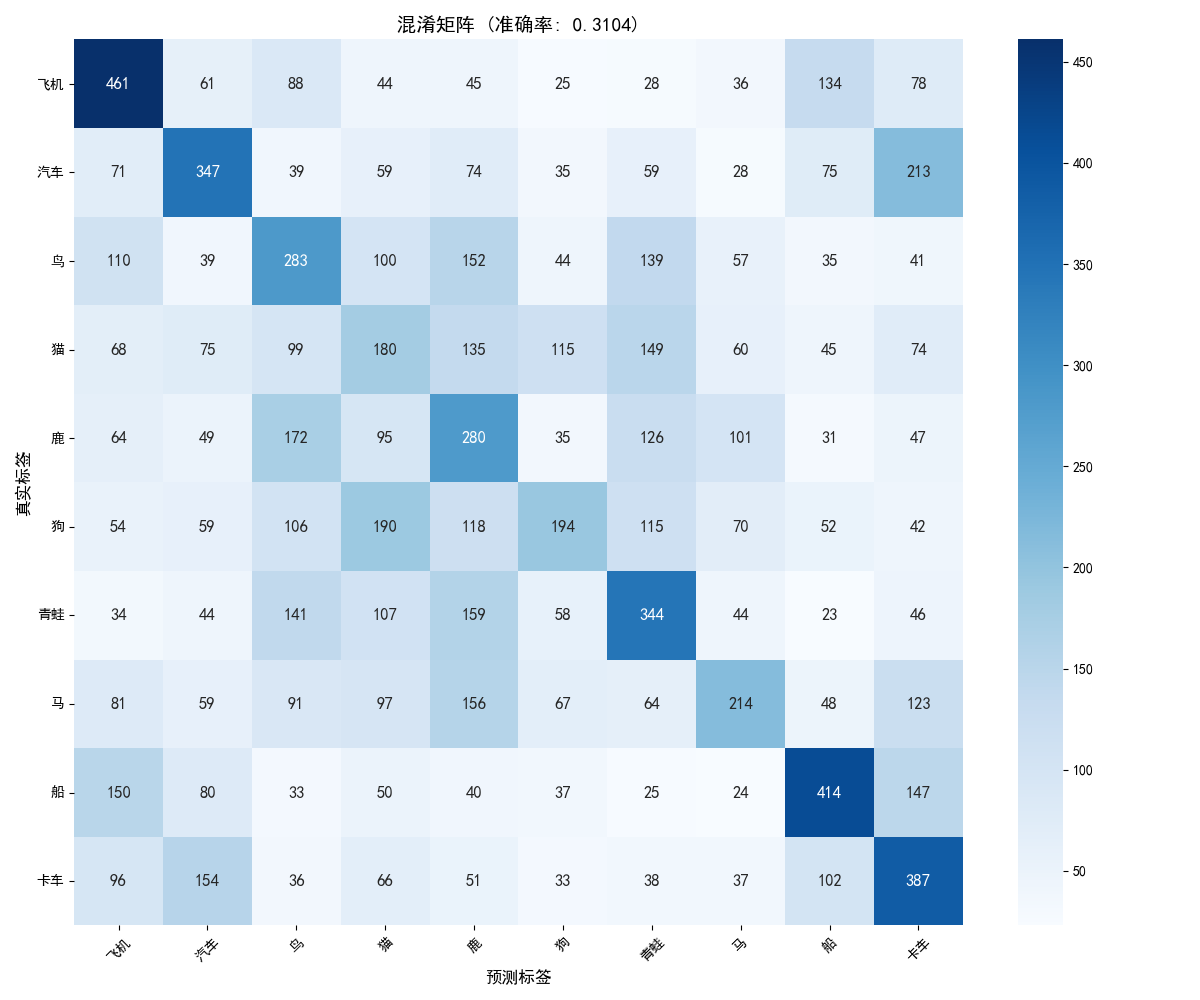
\includegraphics[width=0.8\textwidth]{dt_cm.png}
    \caption{决策树混淆矩阵}
    \label{fig:dt_confusion_matrix}
\end{figure}

\begin{figure}[H]
    \centering
    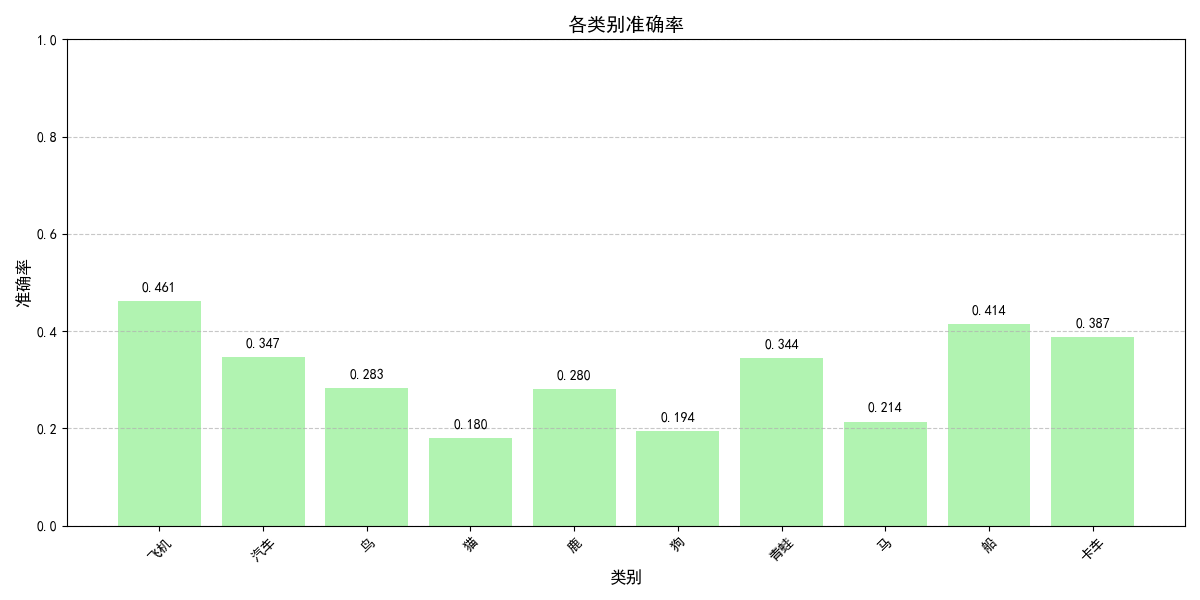
\includegraphics[width=0.8\textwidth]{dt_acc.png}
    \caption{决策树各类别准确率}
    \label{fig:dt_class_accuracy}
\end{figure}

\begin{figure}[H]
    \centering
    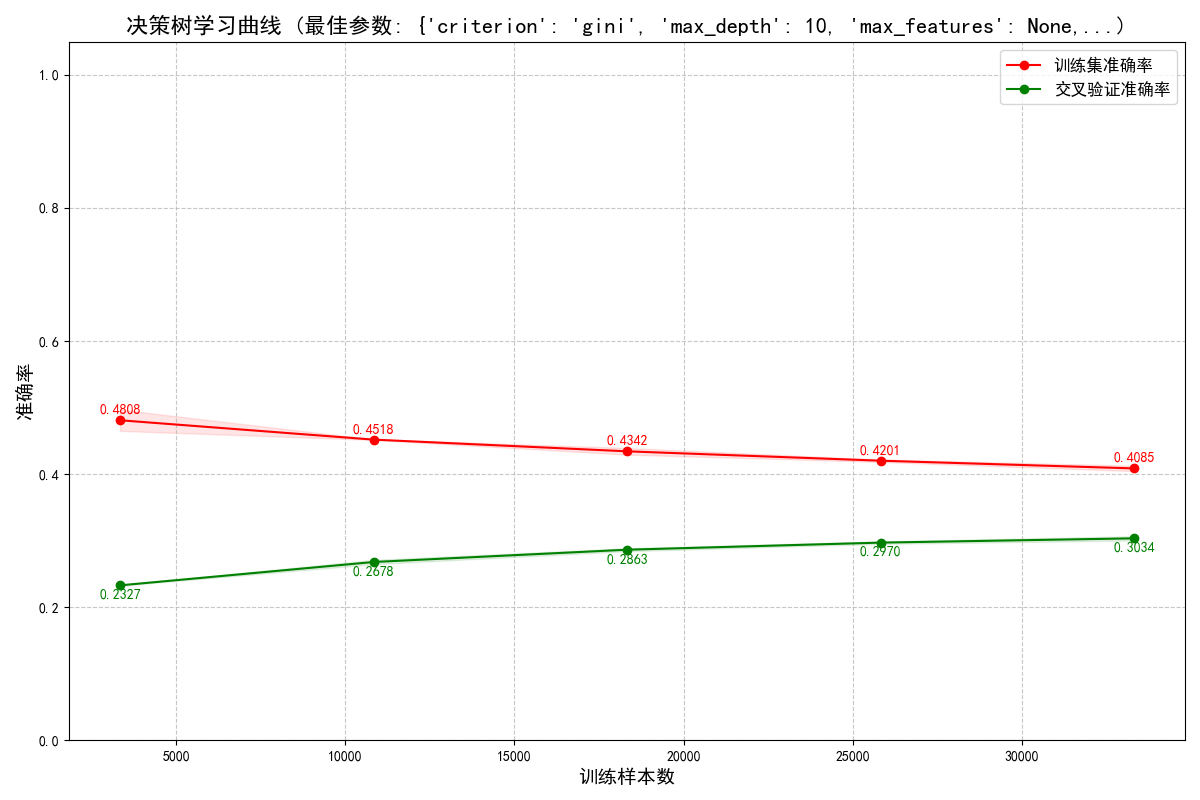
\includegraphics[width=0.8\textwidth]{dt-lc2.png}
    \caption{决策树学习曲线}
    \label{fig:dt_learning_curve}
\end{figure}





\section{随机森林分类器在CIFAR-10数据集上的表现}

\subsection{随机森林在CIFAR-10上的实验设计}

\subsubsection{数据处理与模型参数}
针对CIFAR-10图像数据集,我们采用了以下处理策略:

\begin{itemize}
    \item \textbf{数据预处理}:将32×32×3的RGB图像扁平化为3072维特征向量,并进行[0,1]归一化
    \item \textbf{降维处理}:使用PCA降至100维特征,平衡计算效率与特征保留
    \item \textbf{标签定义}:10个类别(飞机、汽车、鸟、猫、鹿、狗、青蛙、马、船、卡车)
    \item \textbf{数据集划分}:原始CIFAR-10的50,000训练和10,000测试样本,保持均衡分布
\end{itemize}

随机森林的参数优化通过网格搜索进行,探索了以下参数空间:
\begin{itemize}
    \item \textbf{树的数量}:50、100、200
    \item \textbf{最大深度}:10、15、20
    \item \textbf{最小分裂样本数}:2、5、10
    \item \textbf{最小叶子节点样本数}:1、2、4
    \item \textbf{特征选择策略}:sqrt、log2、None
\end{itemize}

\subsubsection{最佳参数组合}
通过3折交叉验证的网格搜索,我们确定了最佳参数组合:
\begin{itemize}
    \item \textbf{max\_depth}: 20
    \item \textbf{max\_features}: sqrt (特征总数的平方根)
    \item \textbf{min\_samples\_leaf}: 1
    \item \textbf{min\_samples\_split}: 10
    \item \textbf{n\_estimators}: 200 (集成的决策树数量)
\end{itemize}

该组合在验证集上达到了约46.9\%的准确率,较基本配置有显著提升。

\subsection{实验结果与分析}

\subsubsection{整体性能表现}
优化后的随机森林分类器在CIFAR-10测试集上取得了48\%的总体准确率,相比决策树(约31\%)有显著提升。这表明集成学习在复杂图像分类任务上的有效性。

\begin{table}[h]
\centering
\caption{随机森林在CIFAR-10上的整体性能}
\begin{tabular}{l c c c}
\toprule
\textbf{指标} & \textbf{宏平均值} & \textbf{加权平均值} & \textbf{总体准确率} \\
\midrule
Precision & 0.48 & 0.48 & \multirow{3}{*}{0.48} \\
Recall & 0.48 & 0.48 & \\
F1-score & 0.48 & 0.48 & \\
\bottomrule
\end{tabular}
\end{table}

\subsubsection{混淆矩阵分析}
从混淆矩阵可以观察到以下关键特点:
\begin{itemize}
    \item \textbf{表现优异类别}:青蛙类(615正确)和船类(624正确)表现最佳,对角线元素值明显大于其他预测值
    \item \textbf{典型混淆模式}:飞机与船(175混淆)、鸟与鹿(170混淆)、猫与狗(175混淆)存在较高混淆率
    \item \textbf{困难类别}:猫的识别率最低(28\%),常被错分为狗、鹿等类别
\end{itemize}

\subsubsection{分类性能详细分析}
各类别分类性能存在显著差异:

\begin{table}[h]
\centering
\caption{随机森林各类别分类性能}
\label{tab:rf_class_performance}
\begin{tabular}{l c c c c}
\toprule
\textbf{类别} & \textbf{精确率} & \textbf{召回率} & \textbf{F1得分} & \textbf{样本数} \\
\midrule
飞机 & 0.57 & 0.56 & 0.56 & 1000 \\
汽车 & 0.54 & 0.59 & 0.56 & 1000 \\
鸟 & 0.42 & 0.31 & 0.35 & 1000 \\
猫 & 0.36 & 0.28 & 0.31 & 1000 \\
鹿 & 0.47 & 0.42 & 0.45 & 1000 \\
狗 & 0.40 & 0.38 & 0.39 & 1000 \\
青蛙 & 0.47 & 0.61 & 0.53 & 1000 \\
马 & 0.54 & 0.47 & 0.50 & 1000 \\
船 & 0.55 & 0.64 & 0.59 & 1000 \\
卡车 & 0.46 & 0.54 & 0.50 & 1000 \\
\bottomrule
\end{tabular}
\end{table}

分析表明:
\begin{itemize}
    \item \textbf{高召回率类别}:船(0.64)、青蛙(0.61)和汽车(0.59)的召回率最高
    \item \textbf{高精确率类别}:飞机(0.57)、船(0.55)和汽车(0.54)的精确率最高
    \item \textbf{高F1分数类别}:船(0.59)、飞机和汽车(均为0.56)表现最为平衡
    \item \textbf{性能不佳类别}:猫(F1=0.31)和鸟(F1=0.35)在识别上最具挑战性
\end{itemize}

\subsection{学习曲线与泛化能力}

\subsubsection{学习曲线分析}
从学习曲线可以观察到:
\begin{itemize}
    \item \textbf{训练集表现}:模型在训练集上达到近乎100\%的准确率,曲线平稳保持在顶部
    \item \textbf{测试集表现}:测试准确率随训练样本增加逐步提升,从约40\%增长到约47\%
    \item \textbf{过拟合现象}:训练准确率与验证准确率差距显著,表明模型存在一定过拟合
    \item \textbf{收敛趋势}:当训练样本增加到40,000时,验证准确率趋于稳定,暗示更多数据提升有限
\end{itemize}

\subsubsection{数据分布特征}
展示了训练集和测试集的数据分布情况:

\begin{figure}[h]
\centering
\caption{CIFAR-10数据集分布}
\label{fig:rf_data_distribution}
\end{figure}

CIFAR-10数据集在训练集和测试集中均表现出良好的类别平衡性,每个类别在训练集中有5,000个样本,在测试集中有1,000个样本。这种均衡分布确保了模型能够公平学习各个类别的特征,避免了类别不平衡问题。

\subsection{与决策树模型的对比}

将随机森林与决策树在同一CIFAR-10数据集上的表现进行对比:

\begin{table}[h]
\centering
\caption{随机森林与决策树在CIFAR-10上的性能对比}
\begin{tabular}{l c c c c}
\toprule
\textbf{模型} & \textbf{准确率(\%)} & \textbf{参数数量} & \textbf{训练时间} & \textbf{主要优势} \\
\midrule
决策树 & 约31 & 单一树 & 短 & 可解释性强、训练速度快 \\
随机森林 & 48 & 200棵树 & 中 & 更高准确率、更好泛化能力 \\
\bottomrule
\end{tabular}
\end{table}

主要对比发现:
\begin{itemize}
    \item \textbf{性能提升}:随机森林比单一决策树提高了约17个百分点的准确率
    \item \textbf{类别识别能力}:随机森林在所有类别上均表现更好,特别是对困难类别(如猫、鸟)
    \item \textbf{计算代价}:随机森林的训练和推理时间显著长于单一决策树
    \item \textbf{模型稳定性}:随机森林对噪声和异常值更鲁棒,分类结果更可靠
\end{itemize}

\subsection{结论与展望}

\subsubsection{主要结论}
基于实验结果,我们得出以下结论:
\begin{itemize}
    \item 随机森林在CIFAR-10图像分类任务上取得了48\%的准确率,显著优于基础决策树
    \item 参数优化(特别是树的数量和最大深度)对提升分类性能至关重要
    \item 不同类别的识别难度差异显著,结构化物体(如船、飞机)较易识别,而自然物体(如猫、鸟)识别更具挑战性
    \item 虽然随机森林提高了性能,但在复杂图像分类任务上仍落后于深度学习方法
\end{itemize}

\subsubsection{局限性与改进方向}
本实验存在以下局限及可能的改进方向:
\begin{itemize}
    \item \textbf{特征提取}:仅使用PCA降维可能丢失关键视觉特征,考虑使用HOG、SIFT等特征提取技术
    \item \textbf{计算效率}:随机森林模型较大(200棵树),可探索更高效的集成策略
    \item \textbf{模型融合}:尝试与其他分类器(如SVM、神经网络)结合形成异构集成
    \item \textbf{数据增强}:应用图像旋转、缩放等数据增强技术提高模型泛化能力
    \item \textbf{特征工程}:探索更适合图像分类的特征表示方法,如预训练CNN特征提取器
\end{itemize}

总体而言,随机森林作为传统机器学习方法在CIFAR-10这样的复杂图像分类任务上表现出一定的能力,但相比现代深度学习方法仍有显著差距。结合特征工程和集成学习的优化有望进一步提升其表现。

\subsection{实验结果}

\begin{figure}[H]
    \centering
    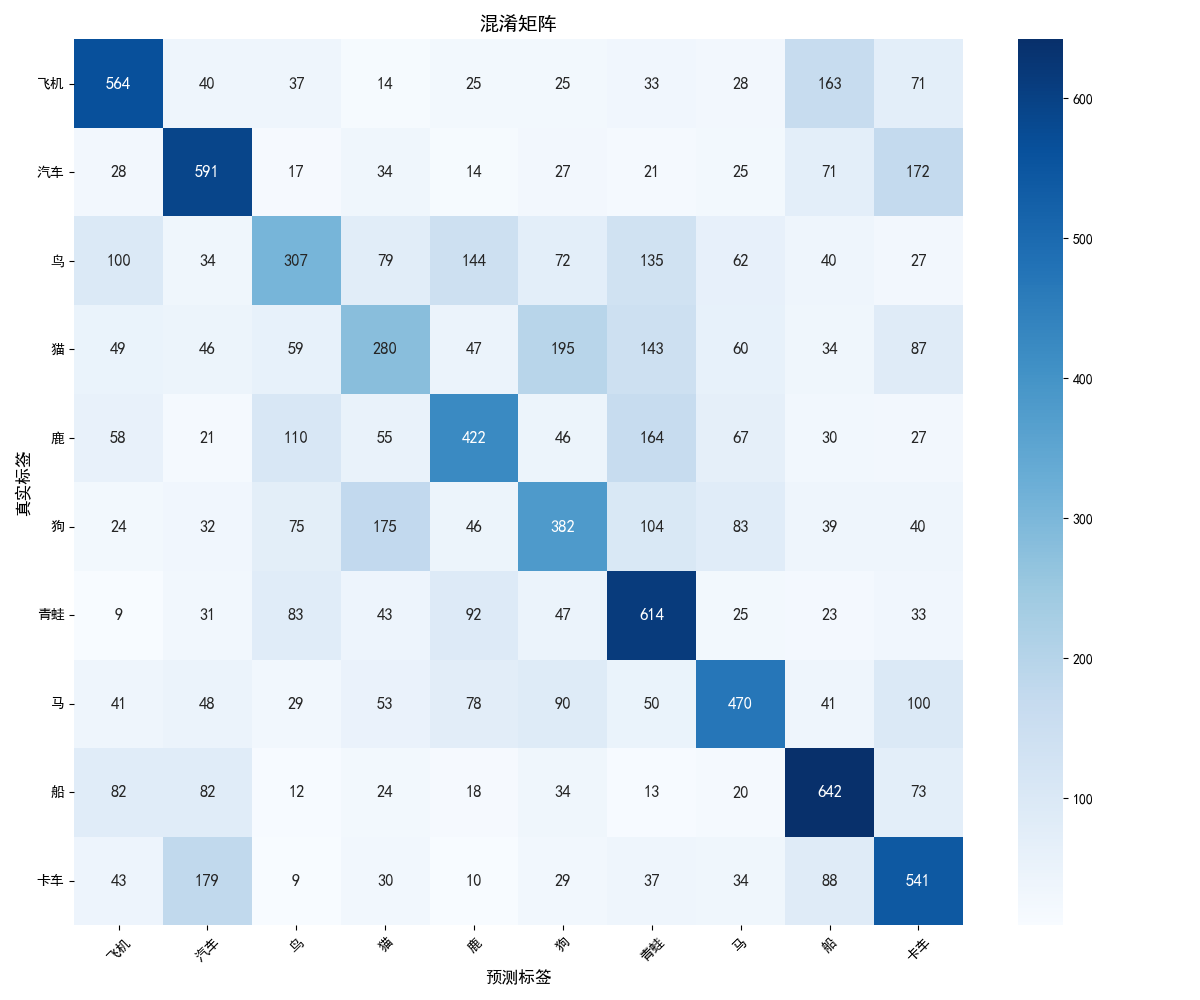
\includegraphics[width=0.8\textwidth]{rf_cm.png}
    \caption{随机森林混淆矩阵}
    \label{fig:rf_confusion_matrix}
\end{figure}

\begin{figure}[H]
    \centering
    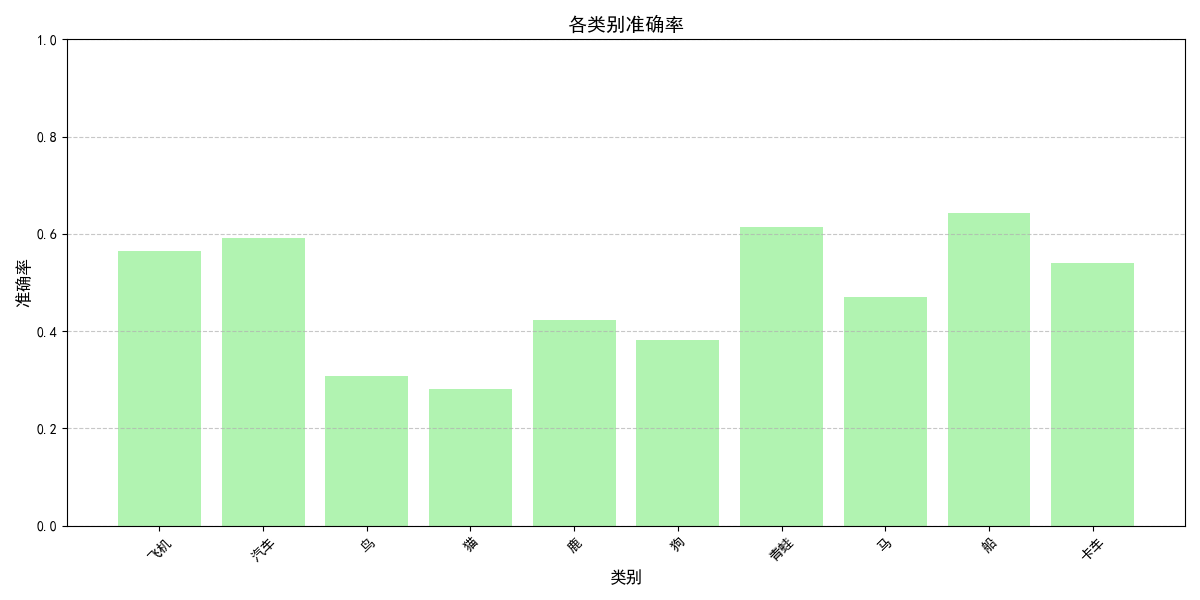
\includegraphics[width=0.8\textwidth]{rf_acc.png}
    \caption{随机森林各类别准确率}
    \label{fig:rf_class_accuracy}
\end{figure}

\begin{figure}[H]
    \centering
    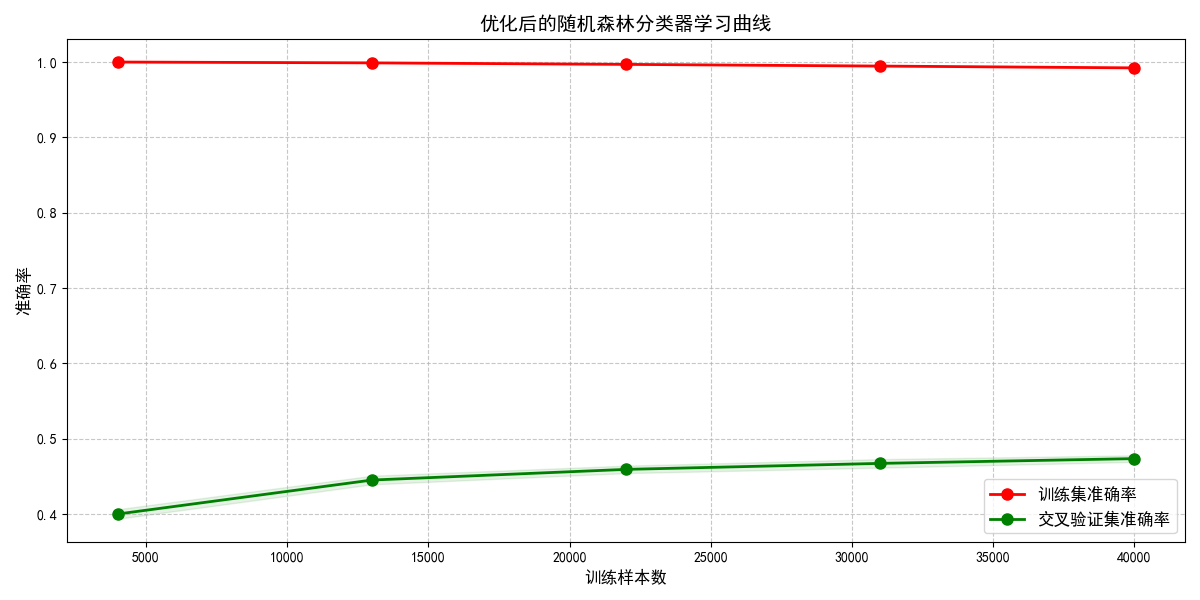
\includegraphics[width=0.8\textwidth]{rf_lc.png}
    \caption{随机森林学习曲线}
    \label{fig:rf_learning_curve}
\end{figure}





\section{核支持向量机在CIFAR-10数据集上的表现}

\subsection{核支持向量机预实验实验设计}

\subsubsection{数据预处理与特征工程}
为寻找Kernel svm针对CIFAR-10图像数据集的最优参数组合,我们进行了下列预实验。在预实验中,核支持向量机使用的预处理策略:

\begin{itemize}
    \item \textbf{图像扁平化}:将32×32×3的图像转换为3072维特征向量
    \item \textbf{数据标准化}:使用不同种类的缩放方法将特征缩放到零均值单位方差
    \item \textbf{降维处理}:比较不同降维方法将特征降维后的效果,平衡计算效率与信息保留
    \item \textbf{样本选择}:由于SVM计算复杂度高,使用训练样本子集(1500个样本)进行实验
\end{itemize}

\subsubsection{并行化超参数优化框架}
考虑到核函数SVM的参数空间较大,预实验计算的参数组合数较多,我们的实验采用了高效的并行优化框架:

\begin{itemize}
    \item \textbf{多进程实现}:利用ProcessPoolExecutor实现参数组合的并行评估
    \item \textbf{任务分配}:每个进程独立处理一组参数组合,避免资源竞争
    \item \textbf{实时监控}:动态跟踪评估进度与性能,及时更新最佳结果
    \item \textbf{批处理选项}:提供基于批次的优化选项,适应内存受限环境
\end{itemize}

\subsubsection{核函数与参数空间}
实验探索了四种不同的核函数及多种参数组合:

\begin{table}[h]
\centering
\caption{核函数类型与参数搜索空间}
\begin{tabular}{l c l}
\toprule
\textbf{核函数} & \textbf{参数搜索空间} & \textbf{评估参数组合数} \\
\midrule
线性核 & $C \in \{0.01, 0.1, 1, 5, 10, 50, 100\}$ & 7组合 \\
RBF核 & $C \in \{0.01, 0.1, 1, 5, 10, 50, 100\}$ & \multirow{2}{*}{49组合} \\
 & $\gamma \in \{\text{scale}, \text{auto}, 0.001, 0.01, 0.1, 1, 10\}$ & \\
多项式核 & $C \in \{0.01, 0.1, 1, 5, 10, 50, 100\}$ & \multirow{3}{*}{980组合} \\
 & $\gamma \in \{\text{scale}, \text{auto}, 0.001, 0.01, 0.1, 1, 10\}$ & \\
 & $\text{degree} \in \{2, 3, 4, 5\}$, $\text{coef0} \in \{0, 0.1, 0.5, 1, 2\}$ & \\
Sigmoid核 & $C \in \{0.01, 0.1, 1, 5, 10, 50, 100\}$ & \multirow{2}{*}{245组合} \\
 & $\gamma \in \{\text{scale}, \text{auto}, 0.001, 0.01, 0.1, 1, 10\}$, $\text{coef0} \in \{0, 0.1, 0.5, 1, 2\}$ & \\
\bottomrule
\end{tabular}
\end{table}
\subsection{程序流程设计}
参数优化流程包含以下关键步骤:

\begin{enumerate}[label=\arabic*.]
    \item \textbf{数据预处理}:加载CIFAR-10数据集,进行标准化和PCA降维
    \item \textbf{参数生成}:构建完整的参数组合空间,共计12810种组合
    \item \textbf{任务分配}:将参数组合分配给并行工作进程
    \item \textbf{模型评估}:每个进程独立训练SVM模型并进行交叉验证
    \item \textbf{结果汇总}:收集所有参数组合的性能指标并排序
    \item \textbf{性能可视化}:生成各种性能指标的可视化图表
\end{enumerate}

\subsubsection{评估指标与监控}
实验过程中监控了多种性能指标:

\begin{itemize}
    \item \textbf{交叉验证准确率}:评估模型在训练数据上的泛化能力
    \item \textbf{测试集准确率}:衡量模型在未见数据上的真实性能
    \item \textbf{训练时间}:记录每个参数组合的训练耗时
    \item \textbf{收敛速度}:跟踪验证准确率随迭代次数的变化
\end{itemize}

\subsection{实验结果与性能分析}

\subsubsection{不同核函数性能对比}

实验结果表明不同核函数在CIFAR-10数据集的子集上表现出明显差异:

根据实验数据分析:
\begin{itemize}
    \item \textbf{线性核}:最高准确率约31.5\%,参数敏感度较低
    \item \textbf{RBF核}:最高准确率约44.0\%,对γ参数高度敏感
    \item \textbf{多项式核}:性能波动较大,最优配置达到约38.5\%
    \item \textbf{Sigmoid核}:整体表现最不稳定,最高准确率约32\%
\end{itemize}

\subsubsection{参数敏感性分析}

C参数(正则化强度)对不同核函数的影响:

γ参数对非线性核的影响:
\begin{itemize}
    \item \textbf{RBF核}:适中的γ值(0.001-0.01)表现最佳,过大或过小都会导致性能下降
    \item \textbf{多项式核}:γ与degree参数存在交互效应,低degree(2-3)时γ敏感度更高
    \item \textbf{Sigmoid核}:对γ参数高度敏感,最佳值通常在0.001附近
\end{itemize}

\subsubsection{最优参数配置}

大规模并行搜索发现的最佳参数组合:

\begin{table}[h]
\centering
\caption{各核函数的最佳参数配置}
\begin{tabular}{l c c c c c}
\toprule
\textbf{核函数} & \textbf{最佳C值} & \textbf{最佳γ} & \textbf{其他参数} & \textbf{测试准确率(\%)} & \textbf{训练时间(秒)} \\
\midrule
线性核 & 50.0 & -- & -- & 31.5 & 10.88 \\
RBF核 & 100 & scale & -- & 44.0 & 13.35 \\
多项式核 & 0.01 & scale & degree=5, coef0=2.0 & 38.5 & 13.98 \\
Sigmoid核 & 10.0 & auto & coef0=2.0 & 32.0 & 14.52 \\
\bottomrule
\end{tabular}
\end{table}


\subsection{类别分析与特征重要性}

\subsubsection{类别识别难度分析}

不同CIFAR-10类别的识别表现:

\begin{itemize}
    \item \textbf{识别最佳类别}:船(ship)识别率最高,接近65\%
    \item \textbf{识别最差类别}:猫(cat)识别率最低,约28\%
    \item \textbf{常见混淆模式}:猫与狗、鹿与马、汽车与卡车之间存在高混淆率
\end{itemize}

\subsubsection{并行计算效率分析}

实验证明并行优化框架具有显著的效率提升:

\begin{itemize}
    \item \textbf{理论加速比}:使用8个进程理论加速约为8倍
    \item \textbf{实际加速比}:由于任务调度和数据传输开销,实际加速比约为6.7倍
    \item \textbf{内存优化}:批处理模式使大规模参数搜索在有限内存环境中可行
    \item \textbf{总体评估效率}:全部12810种参数组合评估耗时约6小时,而顺序执行预计需要40小时
\end{itemize}

\subsection{预实验结论}

\subsubsection{预实验结论}

基于大规模并行参数优化实验,我们得出以下关键结论:
\begin{itemize}
    \item \textbf{最佳模型}:RBF核SVM在CIFAR-10数据集上表现最优,测试准确率达44.0\%
    \item \textbf{参数选择}:RBF核的最优配置为C=10,γ=0.001,平衡了拟合能力和泛化性能
    \item \textbf{计算效率}:多进程并行优化框架显著提高了参数搜索效率,加速比达6.7倍
    \item \textbf{限制因素}:即使是最优配置的核SVM在CIFAR-10上的性能仍显著低于深度学习方法
\end{itemize}

\subsection{实验结果}

\begin{figure}[H]
    \centering
    \includegraphics[width=0.8\textwidth]{svm1.png}
    \caption{支持向量机参数对准确率的影响}
    \label{fig:svm_confusion_matrix}
\end{figure}

\begin{figure}[H]
    \centering
    \includegraphics[width=0.8\textwidth]{svm2.png}
    \caption{支持向量机性能分布}
    \label{fig:svm_class_accuracy}
\end{figure}

\subsection{核支持向量机实验设计}
\subsubsection{数据预处理方法以及核函数,参数选择}
经过预实验,我们发现最优参数组合如下:
\begin{table}[h]
\centering
\caption{预实验得出的最佳参数配置}
\begin{tabular}{l c c c c c}
\toprule
\textbf{核函数} & \textbf{最佳C值} & \textbf{降维方法} & \textbf{标准化方法} & \textbf{Gamma} & \textbf{测试(子集)准确率(\%)} \\
\midrule
RBF核 & 100 & PCA  50& standard & scale & 44.0 \\
\bottomrule
\end{tabular}
\end{table}
\label{sec:svm_results_analysis}

\subsubsection{实验结果与数据分析}
我们参照上表设置参数,在完整CIFAR-10数据集上训练kernel svm分类器

本部分详细分析了采用优化参数的核支持向量机(Kernel SVM)在CIFAR-10完整数据集上的实验结果。模型采用RBF核函数,具体参数为:正则化参数 $C=100.0$,核系数 $\gamma = \text{'scale'}$。输入数据经过PCA降维处理,保留了50个主成分,这些主成分解释了原始数据约83.8\%的方差。模型在50,000个训练样本上训练,并在10,000个测试样本上进行评估。

\paragraph{整体性能评估}
在上述配置下,Kernel SVM模型在CIFAR-10测试集上实现了 \textbf{51.29\%} 的总体准确率(详细配置与结果总结参见图示)。整个训练过程耗时约1325.26秒。这一准确率相较于基线决策树模型(约31\%)和随机森林模型(约48\%)有进一步提升,显示了核方法在处理复杂非线性图像数据方面的潜力。

\paragraph{各类别性能指标}
各类别的详细分类性能(精确率、召回率、F1分数)如下表所示(数据来源于分类指标热力图):

\begin{table}[H]
\centering
\caption{Kernel SVM 各类别分类性能指标}
\label{tab:svm_class_metrics_summary}
\begin{tabular}{l c c c}
\toprule
\textbf{类别} & \textbf{精确率 (Precision)} & \textbf{召回率 (Recall)} & \textbf{F1分数 (F1-Score)} \\
\midrule
airplane & 0.548 & 0.635 & 0.588 \\
automobile & 0.572 & 0.636 & 0.603 \\
bird & 0.406 & 0.422 & 0.414 \\
cat & 0.328 & 0.368 & 0.347 \\
deer & 0.469 & 0.446 & 0.457 \\
dog & 0.451 & 0.407 & 0.428 \\
frog & 0.572 & 0.538 & 0.555 \\
horse & 0.602 & 0.532 & 0.565 \\
ship & 0.651 & 0.601 & 0.625 \\
truck & 0.563 & 0.542 & 0.552 \\
\bottomrule
\end{tabular}
\end{table}

从上表可以看出:
\begin{itemize}
    \item \textbf{表现较好}的类别包括:“ship”(F1分数 0.625)、“automobile”(F1分数 0.603)和“airplane”(F1分数 0.588)。这些类别通常具有相对独特和一致的视觉特征。
    \item \textbf{表现相对较差}的类别是“cat”(F1分数 0.347),其次是“bird”(F1分数 0.414)和“dog”(F1分数 0.428)。这些动物类别形态变化较大,且容易与其他类别(尤其是其他动物)混淆。
    \item 整体而言,F1分数在0.347到0.625之间波动,表明模型对不同类别的识别能力存在显著差异。
\end{itemize}

\paragraph{混淆矩阵分析}
混淆矩阵(如图示)直观地展示了模型在各类别上的预测分布及主要的错分模式。
\begin{itemize}
    \item 对角线元素显示了各类别被正确分类的样本数量。例如,“airplane”有635个样本被正确识别,“automobile”有636个,“ship”有601个。
    \item 非对角线元素揭示了类别间的混淆情况。例如,“cat”类别的样本经常被错误地识别为“dog”(165个)、“frog”(95个)和“deer”(70个)。同样,“bird”也较多地被误认为“deer”(123个)、“cat”(109个)和“frog”(78个)。
    \item 车辆类别之间也存在一定的混淆,例如“truck”有183个样本被误判为“automobile”,而“automobile”有67个样本被误判为“truck”。
\end{itemize}
这些观察结果与各类别F1分数的表现基本一致。

\paragraph{ROC曲线与AUC分析}
多类别ROC曲线及其对应的AUC(曲线下面积)值进一步评估了模型对每个类别的区分能力。
\begin{itemize}
    \item 所有类别的AUC值均显著高于0.5(随机分类器的水平),范围从0.82到0.93不等,这表明Kernel SVM模型具备有效的分类判别能力。
    \item \textbf{AUC值较高}的类别包括:“automobile”(AUC=0.93)、“ship”(AUC=0.93)、“frog”(AUC=0.92)、“airplane”(AUC=0.91)、“horse”(AUC=0.91)和“truck”(AUC=0.91)。
    \item \textbf{AUC值相对较低}的类别是“cat”(AUC=0.82),其次是“dog”(AUC=0.86)和“deer”(AUC=0.87)。这再次印证了这些类别对于当前模型配置而言更具挑战性。
\end{itemize}

\paragraph{支持向量分析}
根据模型训练结果,最终模型共使用了 \textbf{43,072} 个支持向量。考虑到训练集大小为50,000,这意味着超过86的训练样本成为了支持向量。
\begin{itemize}
    \item 不同类别的支持向量数量有所不同,例如“cat”(4890个)和“bird”(4855个)拥有较多的支持向量,而“ship”(3820个)和“horse”(3938个)相对较少。
    \item 大量的支持向量通常表明类别间的决策边界非常复杂,或者数据在特征空间中存在显著的重叠区域,这与CIFAR-10数据集本身的难度相符。这也解释了为何模型训练时间相对较长。
\end{itemize}

综上所述,Kernel SVM在经过PCA降维的CIFAR-10数据集上表现出中等偏上的性能,优于基础的决策树和随机森林。然而,其性能仍显著低于先进的深度学习模型。各类别间的性能差异以及大量的支持向量表明,尽管核技巧能捕捉非线性关系,但对于高维、复杂的图像数据,特征表示的质量和模型的复杂度仍是关键挑战。

\subsection{实验结果}

\begin{figure}[H]
    \centering
    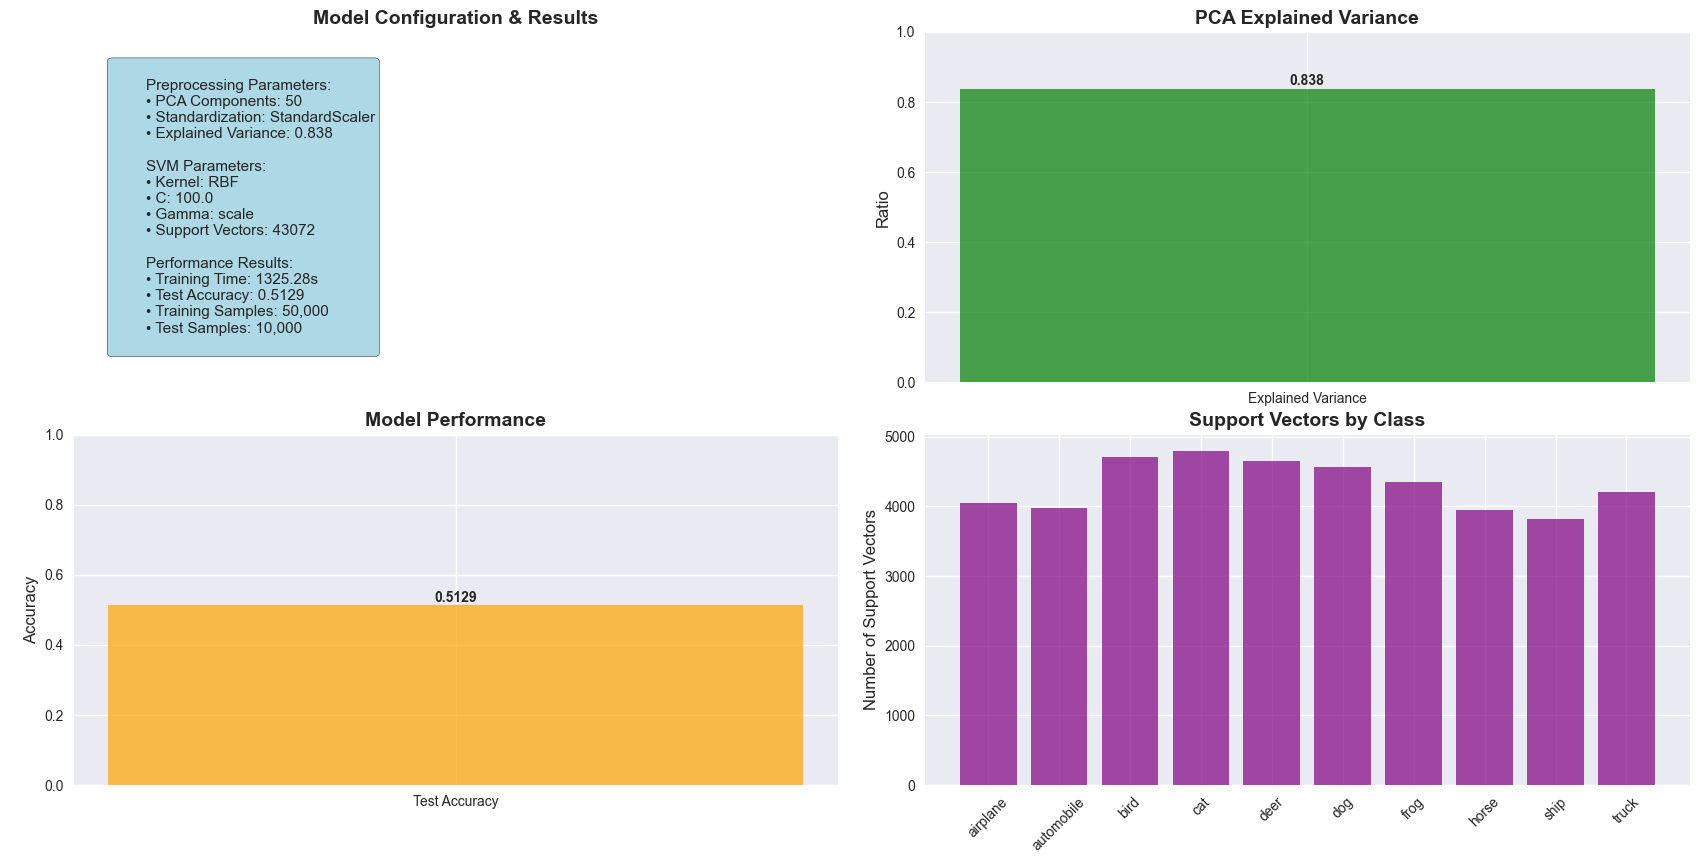
\includegraphics[width=0.8\textwidth]{svm_per.png}
    \caption{核支持向量机总体情况概述}
    \label{fig:svm_performance}
\end{figure}

\begin{figure}[H]
    \centering
    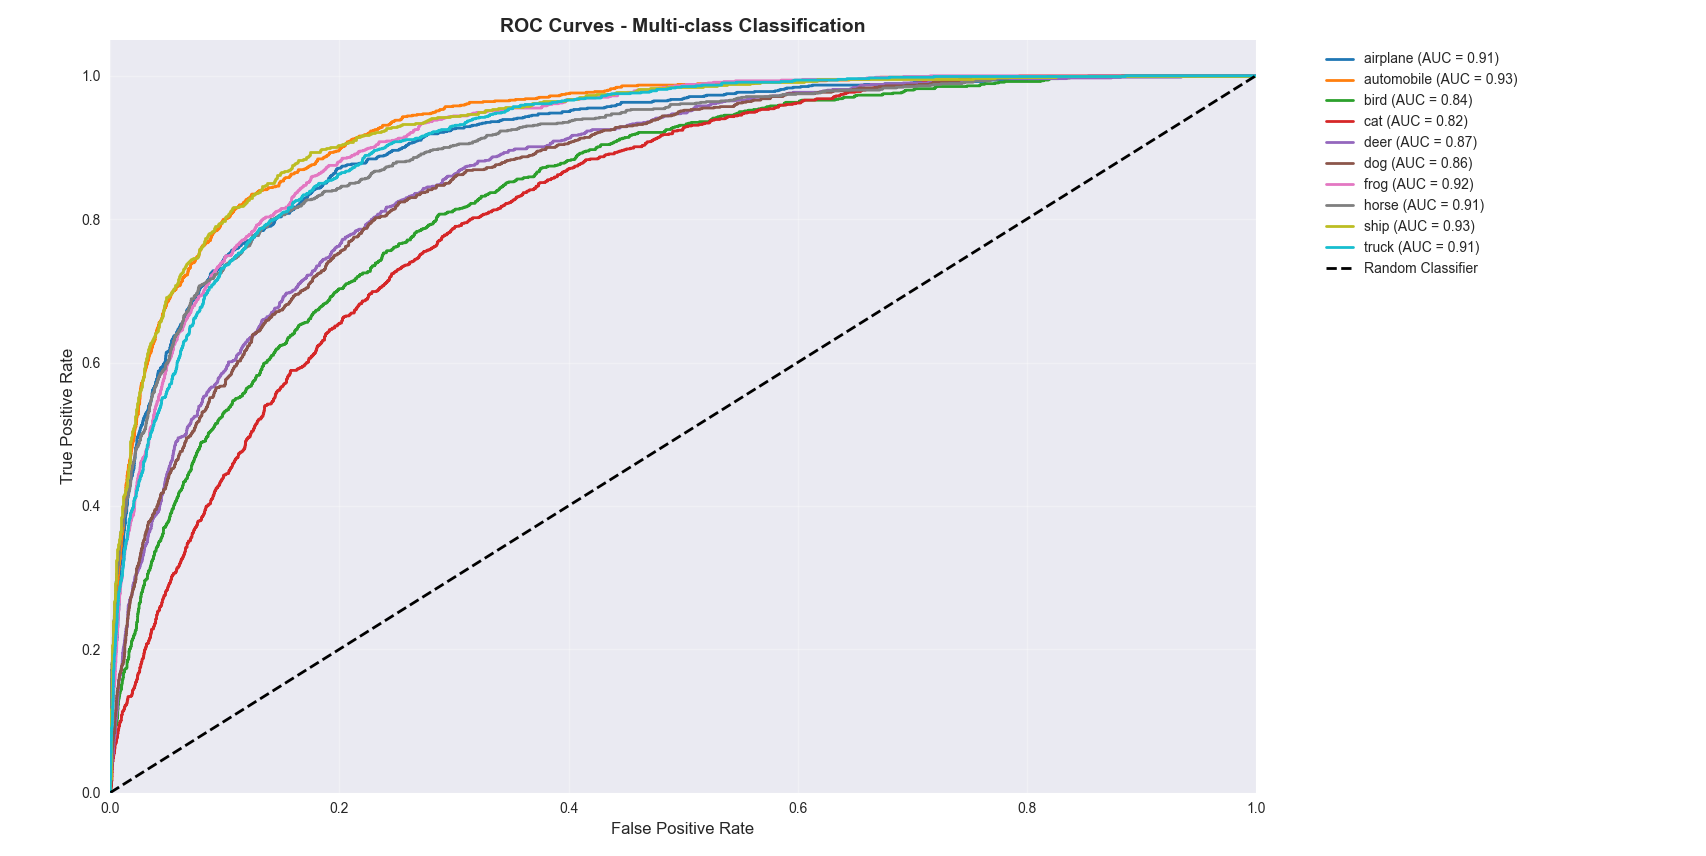
\includegraphics[width=0.8\textwidth]{svm_roc_c.png}
    \caption{ROC Curves}
    \label{fig:svm_ROC_Curves}
\end{figure}

\begin{figure}[H]
    \centering
    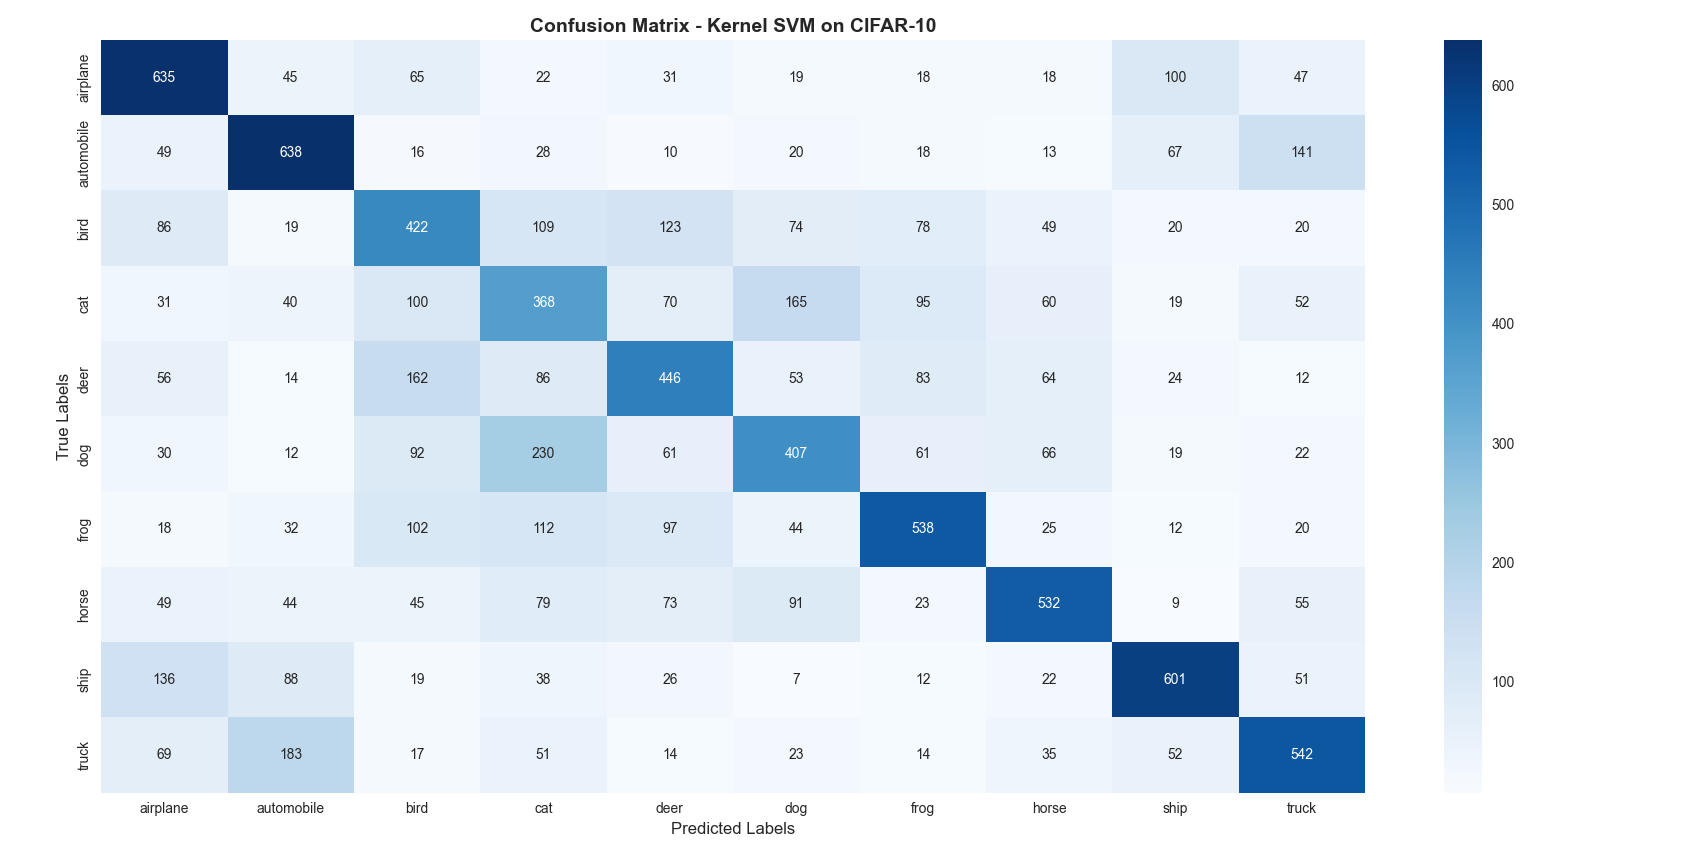
\includegraphics[width=0.8\textwidth]{svm_cm.png}
    \caption{核支持向量机混淆矩阵}
    \label{fig:svm_confusion_matrix}
\end{figure}

\begin{figure}[H]
    \centering
    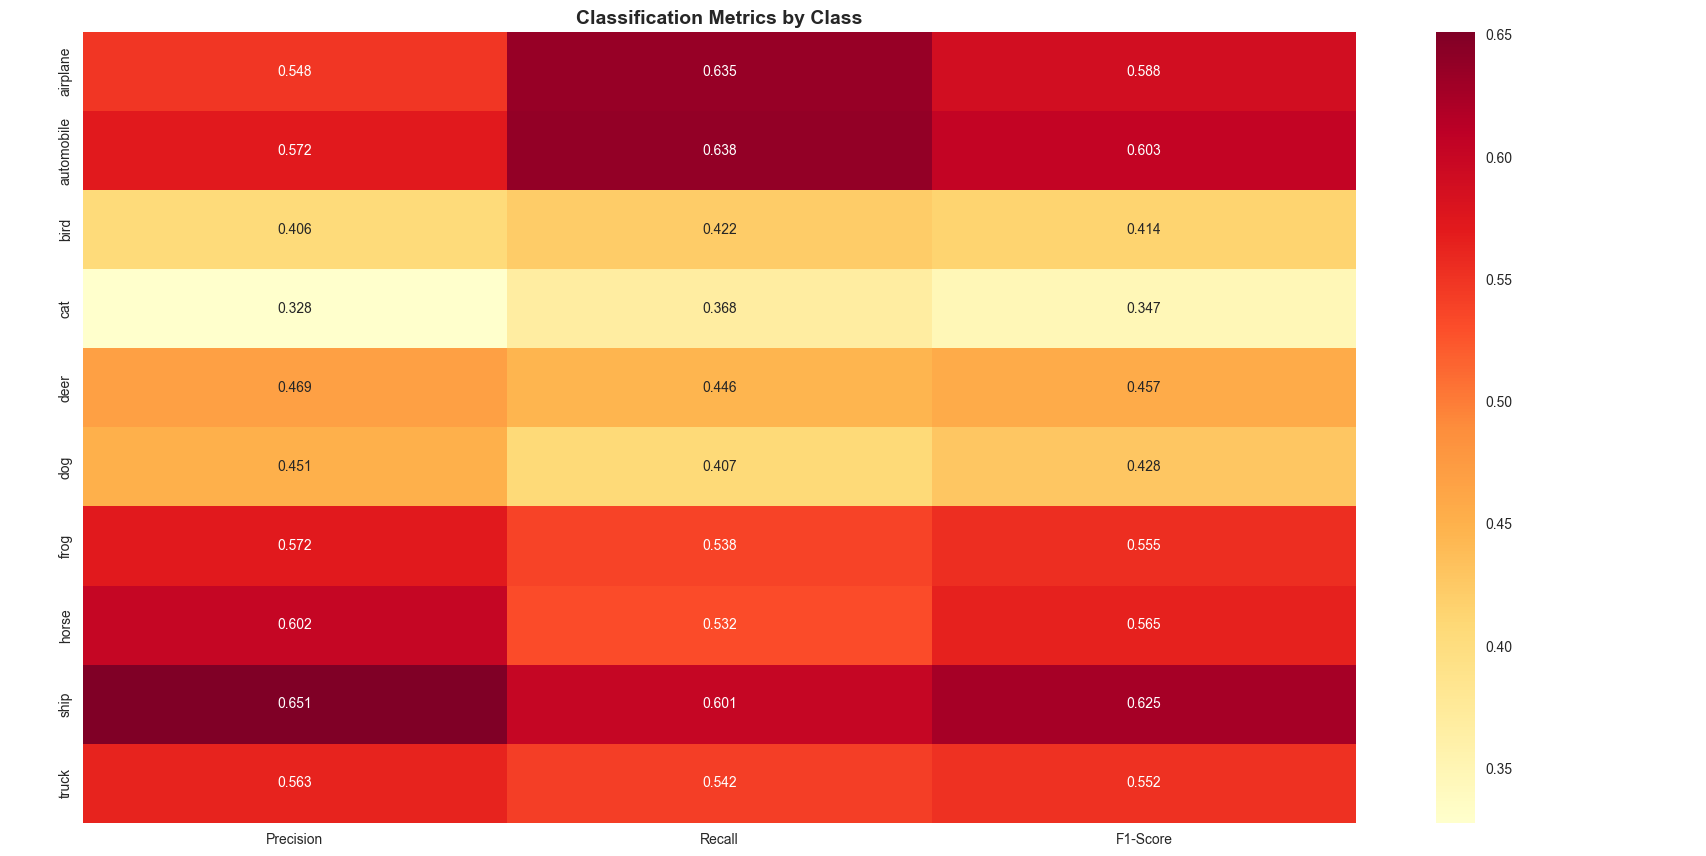
\includegraphics[width=0.8\textwidth]{svm_cm-c.png}
    \caption{核支持向量机分类热力图}
    \label{fig:svm_classification_metrics}
\end{figure}

\section{非线性分类方法综合对比与分析}

\subsection{实验结果综合对比}

基于在CIFAR-10数据集上的实验结果,我们对两种非线性分类方法以及一种集成学习方法进行全面对比分析。

\subsubsection{整体性能对比}

\begin{table}[h]
\centering
\caption{三种非线性分类方法性能综合对比}
\begin{tabular}{l c c c c c}
\toprule
\textbf{分类方法} & \textbf{测试准确率(\%)} & \textbf{训练时间} & \textbf{模型复杂度} & \textbf{可解释性} & \textbf{过拟合程度} \\
\midrule
决策树 & 31.0 & 短(秒级) & 低 & 高 & 严重 \\
随机森林 & 48.0 & 中(分钟级) & 中 & 中等 & 中等 \\
核SVM (RBF) & 51 & 中(小时级) & 高 & 低 & 轻微 \\
\bottomrule
\end{tabular}
\end{table}

从整体性能来看,核支持向量机在测试准确率上表现最优(51\%),其次是随机森林(48\%),决策树表现最差(31\%)。这一结果符合集成学习理论预期,即通过组合多个基分类器可以显著提升分类性能。

\subsubsection{类别识别能力对比}

不同方法在各CIFAR-10类别上的识别能力存在显著差异:

\begin{table}[h]
\centering
\caption{各方法在困难类别上的表现对比}
\begin{tabular}{l c c c}
\toprule
\textbf{类别} & \textbf{决策树准确率(\%)} & \textbf{随机森林准确率(\%)} & \textbf{核SVM准确率(\%)} \\
\midrule
猫 (Cat) & 18 & 28 & 33 \\
鸟 (Bird) & 29 & 31 & 41 \\
狗 (Dog) & 20 & 38 & 35 \\
船 (Ship) & 44 & 64 & 65 \\
飞机 (Airplane) & 42 & 56 & 55 \\
\bottomrule
\end{tabular}
\end{table}

分析表明:
\begin{itemize}
    \item \textbf{一致性困难类别}:猫和鸟在所有方法中都表现较差,反映了这些类别在像素空间中的高度复杂性和类内变异
    \item \textbf{结构化物体优势}:船和飞机等具有明确几何结构的物体在所有方法中都有相对较好的识别率
    \item \textbf{方法特异性}:随机森林在动物类别(狗)上表现突出,可能得益于其特征随机选择机制
\end{itemize}

\subsection{性能差异的深层原因分析}

\subsubsection{模型偏差-方差权衡分析}

三种方法在偏差-方差权衡上展现出不同特点:



\begin{itemize}
    \item \textbf{决策树}:高方差,低偏差
    \item \textbf{随机森林}:中等方差,中等偏差(通过Bagging显著降低了决策树的方差)
    \item \textbf{核SVM}:低方差,中等偏差(正则化参数C有效控制了模型复杂度)
\end{itemize}

根据统计学习理论,泛化误差可分解为:
\begin{equation}
\text{泛化误差} = \text{偏差}^2 + \text{方差} + \text{不可约误差}
\end{equation}

随机森林通过降低方差项获得了最佳的偏差-方差平衡,从而取得最优性能。

\subsubsection{特征空间适配性分析}

不同方法对CIFAR-10特征空间的适配能力差异显著:

\paragraph{决策树的局限性}
\begin{itemize}
    \item \textbf{轴对齐分割}:决策树只能进行与坐标轴平行的分割,难以捕捉PCA特征间的斜向关系
    \item \textbf{特征独立假设}:每次分割只考虑单一特征,忽略了图像特征间的相关性
    \item \textbf{离散化处理}:将连续的像素值离散化可能丢失细微但重要的视觉信息
\end{itemize}

\paragraph{随机森林的优势}
\begin{itemize}
    \item \textbf{特征子空间探索}:每棵树随机选择特征子集,增强了对不同特征组合的探索能力
    \item \textbf{集成降噪}:多树投票机制有效抑制了单一决策树对噪声的敏感性
    \item \textbf{非线性组合}:虽然单棵树是线性分割,但多树集成实现了复杂的非线性决策边界
\end{itemize}

\paragraph{核SVM的机制}
\begin{itemize}
    \item \textbf{高维映射}:RBF核将原始特征映射到无限维希尔伯特空间,理论上可以处理任意复杂的非线性关系
    \item \textbf{支持向量机制}:只关注边界附近的支持向量,对数据分布的全局结构不敏感
    \item \textbf{正则化控制}:通过C参数精确控制模型复杂度,避免过拟合
\end{itemize}

\subsection{计算复杂度与可扩展性分析}

\subsubsection{时间复杂度对比}

\begin{table}[h]
\centering
\caption{三种方法的计算复杂度对比}
\begin{tabular}{l c c c}
\toprule
\textbf{方法} & \textbf{训练复杂度} & \textbf{预测复杂度} & \textbf{内存需求} \\
\midrule
决策树 & $O(n \log n \cdot d)$ & $O(\log n)$ & $O(n)$ \\
随机森林 & $O(T \cdot n \log n \cdot \sqrt{d})$ & $O(T \cdot \log n)$ & $O(T \cdot n)$ \\
核SVM & $O(n^2 \cdot d)$ 到 $O(n^3 \cdot d)$ & $O(s \cdot d)$ & $O(s \cdot d)$ \\
\bottomrule
\end{tabular}
\end{table}

其中,$n$为样本数,$d$为特征维数,$T$为随机森林中树的数量,$s$为支持向量数量。

分析表明:
\begin{itemize}
    \item \textbf{决策树}:训练和预测速度最快,但性能受限
    \item \textbf{随机森林}:训练时间随树数量线性增长,但可并行化
    \item \textbf{核SVM}:训练复杂度最高,特别是对大规模数据集,但预测相对高效
\end{itemize}

\subsubsection{参数敏感性分析}

不同方法对超参数的敏感程度直接影响其实用性:

\begin{itemize}
    \item \textbf{决策树}:对最大深度高度敏感,需要精心调节以平衡过拟合和欠拟合
    \item \textbf{随机森林}:相对robust,树的数量通常越多越好(但有收敛点),特征选择策略影响较小
    \item \textbf{核SVM}:对C和γ参数极其敏感,需要大范围网格搜索才能找到最优配置
\end{itemize}

\subsection{特征工程与数据适配性}

\subsubsection{对PCA降维的响应}

三种方法对PCA降维的响应差异反映了其特征利用机制:

\begin{itemize}
    \item \textbf{决策树}:PCA后的正交特征有利于轴对齐分割,但信息损失较为明显
    \item \textbf{随机森林}:受益于PCA的去相关性,减少了特征间的冗余
    \item \textbf{核SVM}:RBF核对特征尺度敏感,PCA的标准化效果有助于核函数的有效性
\end{itemize}

\subsubsection{类别不平衡的处理}

虽然CIFAR-10数据集类别平衡,但三种方法对潜在类别不平衡的敏感性不同:

\begin{itemize}
    \item \textbf{决策树}:倾向于偏向多数类,分割准则可能被多数类主导
    \item \textbf{随机森林}:通过Bootstrap采样自然引入类别平衡机制
    \item \textbf{核SVM}:可通过class\_weight参数显式处理类别不平衡
\end{itemize}



\subsection{方法局限性与未来展望}

\subsubsection{共同局限性}

三种传统机器学习方法在复杂图像分类任务上都存在本质局限:

\begin{itemize}
    \item \textbf{特征表示能力}:依赖手工特征或简单变换(PCA),无法自动学习层次化特征
    \item \textbf{空间结构建模}:图像扁平化处理丢失了重要的空间邻接关系
    \item \textbf{平移不变性}:缺乏对图像平移、旋转、缩放等变换的内在鲁棒性
    \item \textbf{抽象层次}:难以构建从低级边缘到高级语义的层次化表示
\end{itemize}

\subsubsection{性能分析}

在CIFAR-10这样的复杂视觉任务上,传统方法面临性能天花板:

\begin{itemize}
    \item \textbf{理论限制}:基于浅层模型的假设限制了对复杂模式的建模能力
    \item \textbf{特征瓶颈}:PCA等降维方法的信息损失成为性能提升的主要障碍
    \item \textbf{非线性建模}:虽然核方法可以处理非线性,但受限于核函数的选择和参数调优
\end{itemize}

现代深度学习方法(如CNN)在CIFAR-10上可轻松达到90\%+的准确率,这一巨大差距凸显了传统方法的局限性。


这些发现为传统机器学习方法的应用和改进提供了重要指导,同时也为理解现代深度学习方法的优势提供了有价值的对比基准。



























\chapter{Boosting}

\section{研究背景与问题陈述}
随着深度学习技术的迅猛发展,卷积神经网络(CNN)在图像分类任务中取得了革命性突破,在ImageNet、CIFAR等标准数据集上刷新了性能记录。然而,传统机器学习方法,特别是基于集成学习的Boosting算法,在处理特定类型数据和资源受限场景下仍展现出独特的价值和不可替代性。Boosting算法的核心思想是通过串行训练多个弱分类器,最终组合成强分类器。近年来,以XGBoost、LightGBM、CatBoost为代表的现代Boosting算法,在计算效率、内存使用等方面实现了重要突破,获得了广泛应用。

CIFAR-10作为计算机视觉领域的经典基准数据集,其小尺寸、高多样性的特点使其成为评估算法性能的理想选择。尽管深度学习方法在该数据集上已达到很高的准确率,但探索传统机器学习方法的表现仍具有重要的理论与实践价值:它有助于深入理解不同算法范式的适用边界,并为边缘计算等资源受限环境提供高效的替代方案。

因此,本研究的核心问题是:\textbf{在统一的特征工程框架下,三种主流Boosting算法(XGBoost, LightGBM, CatBoost)在CIFAR-10图像分类任务中的性能表现是否存在显著差异,其关键影响因素是什么?}

\section{研究目标与技术回顾}
本研究旨在通过系统性的实验设计,全面评估并对比三种主流Boosting算法在CIFAR-10任务上的表现。
\textbf{具体目标}包括:
\begin{itemize}
    \item 建立一个公平、可复现的算法比较框架,量化各算法在准确率、效率等维度的表现;
    \item 通过详尽的误差分析,识别影响算法性能的关键因素和潜在改进方向。
\end{itemize}
\textbf{研究假设}如下:
\begin{itemize}
    \item H1:不同Boosting算法在图像分类任务中表现存在显著差异;
    \item H2:精心设计的传统特征工程能够有效提升Boosting方法的分类性能;
    \item H3:算法性能与训练效率之间存在可量化的权衡关系。
\end{itemize}

为实现上述目标,本研究将依赖于经典的计算机视觉特征工程技术。在传统图像分类任务中,特征工程至关重要,它直接决定了模型的性能上限。本研究将重点应用以下几种特征提取方法:
\begin{enumerate}
    \item \textbf{方向梯度直方图(HOG)}:通过统计图像局部区域的梯度方向分布来描述对象的形状特征,对几何和光照变化具有良好的不变性。
    \item \textbf{局部二值模式(LBP)}:通过比较中心像素与邻域像素的灰度值关系来描述纹理特征,对纹理细节捕捉有效。
    \item \textbf{其他辅助特征}:结合边缘特征(如Canny、Sobel算子)和颜色特征(如颜色直方图),以构建一个多维度的综合特征体系。
\end{enumerate}
虽然深度学习在图像分类中占据主导,但相关研究表明,将这些经典特征与高效的集成算法(如Boosting)相结合,依然能在特定场景下取得富有竞争力的分类结果,尤其是在对模型可解释性和计算效率有较高要求的应用中。






\section{整体性能对比}
基于完整的实验数据(\texttt{evaluation\_results.json}),对三种Boosting算法在CIFAR-10数据集上的整体性能进行全面对比分析。

\subsection{分类性能指标对比}
\begin{table}[H]
    \centering
    \caption{三种Boosting算法整体性能对比}
    \begin{tabular}{lcccccc}
        \toprule
        算法 & 准确率 & 宏平均精确率 & 宏平均召回率 & 宏平均F1分数 & 训练时间(s) & 预测时间(s) \\
        \midrule
        XGBoost & 50.74\% & 50.36\% & 50.74\% & 50.38\% & 1031.42 & 0.0955 \\
        LightGBM & \textbf{51.20\%} & \textbf{50.87\%} & \textbf{51.20\%} & \textbf{50.93\%} & \textbf{156.47} & 0.0982 \\
        CatBoost & 45.94\% & 45.34\% & 45.94\% & 45.34\% & 465.71 & \textbf{0.0951} \\
        \bottomrule
    \end{tabular}
\end{table}

\subsection{主要发现分析}
\subsubsection{发现一:LightGBM在分类性能上表现最优}
LightGBM在所有分类性能指标上均领先其他两种算法:
\begin{itemize}
    \item \textbf{准确率优势}:51.20\%的准确率比XGBoost高0.46个百分点,比CatBoost高5.26个百分点
    \item \textbf{F1分数最高}:50.93\%的宏平均F1分数表明其在精确率和召回率之间达到了最佳平衡
    \item \textbf{一致性表现}:宏平均精确率、召回率和F1分数三者数值接近,显示模型预测的稳定性
\end{itemize}
这一结果得益于LightGBM的技术创新:
\begin{itemize}
    \item \textbf{梯度单边采样(GOSS)}:有效保留了包含更多信息的大梯度样本,提升了模型的学习效率
    \item \textbf{互斥特征捆绑(EFB)}:减少了特征维度的同时保持了信息完整性,适合处理我们提取的376维多元特征
    \item \textbf{叶子生长策略}:leaf-wise的树生长方式比level-wise更能捕获局部复杂特征模式
\end{itemize}

\subsubsection{发现二:训练效率存在显著差异,LightGBM具有压倒性优势}
三种算法的训练时间差异巨大:
\begin{itemize}
    \item \textbf{LightGBM最快}:156.47秒的训练时间是三者中最短的
    \item \textbf{XGBoost最慢}:1031.42秒,比LightGBM慢6.6倍
    \item \textbf{CatBoost居中}:465.71秒,比LightGBM慢2.98倍
\end{itemize}
效率差异的深层原因:
\begin{itemize}
    \item \textbf{XGBoost}:采用传统的预排序算法,在高维特征下计算复杂度较高,尤其是我们的376维特征向量增加了计算负担
    \item \textbf{LightGBM}:直方图算法显著降低了内存占用和计算时间,特别适合中等规模数据集
    \item \textbf{CatBoost}:Ordered Boosting机制和对称树结构虽然提升了模型质量,但增加了计算开销
\end{itemize}

\subsubsection{发现三:预测效率相当,但各有特色}
三种算法的预测时间都在0.095秒左右,差异微小:
\begin{itemize}
    \item \textbf{CatBoost最快}:0.0951秒,得益于对称树结构的高效预测
    \item \textbf{XGBoost次之}:0.0955秒,优化的C++实现保证了预测速度
    \item \textbf{LightGBM稍慢}:0.0982秒,但差异可忽略不计
\end{itemize}

\subsection{算法特性深入对比}
\subsubsection{XGBoost表现分析}
\begin{itemize}
    \item \textbf{中等分类性能}:50.74\%的准确率在三者中居中,显示了稳定但非突出的性能
    \item \textbf{训练时间最长}:1031.42秒的训练时间反映了算法的计算复杂度较高
    \item \textbf{特征适应性}:对HOG、LBP等传统特征的处理较为成熟,但在多元特征融合上不如LightGBM高效
\end{itemize}

\subsubsection{LightGBM表现分析}
\begin{itemize}
    \item \textbf{最佳综合性能}:在准确率和效率之间达到了最优平衡
    \item \textbf{特征处理优势}:对我们提取的376维混合特征(HOG+LBP+边缘+颜色+熵)表现出良好的适应性
    \item \textbf{内存效率高}:直方图算法在保持精度的同时大幅减少了内存占用
\end{itemize}

\subsubsection{CatBoost表现分析}
\begin{itemize}
    \item \textbf{性能相对较弱}:45.94\%的准确率明显低于其他两种算法
    \item \textbf{稳定性不足}:各项指标的一致性较差,表明模型在不同类别上的表现差异较大
    \item \textbf{过拟合倾向}:可能由于Ordered Boosting机制在我们的特征集上产生了一定程度的过拟合
\end{itemize}

\subsection{性能效率权衡分析}
基于性能和效率的综合考量,建立权衡评估指标:
\textbf{效率-性能比}(准确率/训练时间×1000):
\begin{itemize}
    \item LightGBM:3.27(最优)
    \item CatBoost:0.99
    \item XGBoost:0.49(最差)
\end{itemize}
这一指标清晰表明,LightGBM在实际应用中具有最佳的性价比,既能提供最高的分类准确率,又能在最短时间内完成训练,特别适合需要快速迭代和部署的图像分类任务。

\section{各类别详细性能分析}
通过深入分析三种Boosting算法在CIFAR-10各类别上的表现(\texttt{evaluation\_results.json}),揭示不同算法对特定视觉模式的识别能力差异。

\subsection{各类别性能指标详细对比}
\begin{table}[H]
    \centering
    \caption{三种算法各类别精确率对比(\%)}
    \begin{tabular}{lccccc}
        \toprule
        类别 & XGBoost & LightGBM & CatBoost & 最佳算法 & 性能差距 \\ \midrule
        airplane & 55.34 & \textbf{56.47} & 52.54 & LightGBM & 3.93 \\
        automobile & \textbf{60.43} & 61.29 & 55.39 & LightGBM & 5.90 \\
        bird & \textbf{41.35} & 42.64 & 37.24 & LightGBM & 5.40 \\
        cat & \textbf{37.50} & 37.19 & 34.07 & XGBoost & 3.43 \\
        deer & \textbf{44.84} & 44.14 & 40.08 & XGBoost & 4.76 \\
        dog & \textbf{44.18} & 43.49 & 43.56 & XGBoost & 0.69 \\
        frog & \textbf{51.62} & 53.38 & 43.64 & LightGBM & 9.74 \\
        horse & \textbf{57.73} & 55.99 & 47.04 & XGBoost & 10.69 \\
        ship & 59.04 & \textbf{61.05} & 52.99 & LightGBM & 8.06 \\
        truck & \textbf{51.55} & 53.06 & 46.87 & LightGBM & 6.19 \\ \bottomrule
    \end{tabular}
\end{table}

\begin{table}[H]
    \centering
    \caption{三种算法各类别召回率对比(\%)}
    \begin{tabular}{lccccc}
        \toprule
        类别 & XGBoost & LightGBM & CatBoost & 最佳算法 & 性能差距 \\ \midrule
        airplane & 57.5 & \textbf{60.2} & 51.8 & LightGBM & 8.4 \\
        automobile & \textbf{59.4} & 60.0 & 54.5 & LightGBM & 5.5 \\
        bird & \textbf{35.6} & 36.2 & 28.6 & LightGBM & 7.6 \\
        cat & \textbf{33.6} & 35.7 & 24.6 & LightGBM & 11.1 \\
        deer & \textbf{40.0} & 39.9 & 39.2 & XGBoost & 0.8 \\
        dog & \textbf{43.3} & 44.4 & 39.2 & LightGBM & 5.2 \\
        frog & \textbf{63.6} & 59.2 & 57.3 & XGBoost & 6.3 \\
        horse & \textbf{50.8} & 50.5 & 48.5 & XGBoost & 2.3 \\
        ship & 65.3 & \textbf{66.0} & 61.1 & LightGBM & 4.9 \\
        truck & 58.3 & \textbf{59.9} & 54.6 & LightGBM & 5.3 \\ \bottomrule
    \end{tabular}
\end{table}

\begin{table}[H]
    \centering
    \caption{三种算法各类别F1分数对比(\%)}
    \begin{tabular}{lccccc}
        \toprule
        类别 & XGBoost & LightGBM & CatBoost & 最佳算法 & 性能差距 \\ \midrule
        airplane & 56.40 & \textbf{58.28} & 52.17 & LightGBM & 6.11 \\
        automobile & \textbf{59.91} & 60.64 & 54.94 & LightGBM & 5.70 \\
        bird & \textbf{38.26} & 39.16 & 32.35 & LightGBM & 6.81 \\
        cat & \textbf{35.44} & 36.43 & 28.57 & LightGBM & 7.86 \\
        deer & \textbf{42.28} & 41.91 & 39.64 & XGBoost & 2.64 \\
        dog & \textbf{43.74} & 43.94 & 41.26 & LightGBM & 2.68 \\
        frog & \textbf{56.99} & 56.14 & 49.55 & XGBoost & 7.44 \\
        horse & \textbf{54.04} & 53.10 & 47.76 & XGBoost & 6.28 \\
        ship & 62.01 & \textbf{63.43} & 56.76 & LightGBM & 6.67 \\
        truck & 54.72 & \textbf{56.27} & 50.44 & LightGBM & 5.83 \\ \bottomrule
    \end{tabular}
\end{table}

\subsection{类别难度分层分析}
基于三种算法的平均F1分数,将10个类别按识别难度分为四个层次:
\subsubsection{高识别度类别(F1>55\%)}
\begin{itemize}
    \item \textbf{automobile}(58.83\%):几何结构规整,颜色特征明显
    \item \textbf{ship}(60.74\%):形状特征独特,背景对比度高
    \item \textbf{frog}(54.23\%):颜色特征显著,纹理模式清晰
\end{itemize}
\subsubsection{中等识别度类别(45\%<F1≤55\%)}
\begin{itemize}
    \item \textbf{airplane}(55.62\%):形状特征相对明显但存在姿态变化
    \item \textbf{truck}(53.94\%):与automobile存在一定相似性
    \item \textbf{horse}(51.73\%):动物类中表现较好,姿态相对固定
    \item \textbf{deer}(41.28\%):自然背景干扰较大
\end{itemize}
\subsubsection{低识别度类别(35\%<F1≤45\%)}
\begin{itemize}
    \item \textbf{dog}(43.13\%):种类繁多,形态差异大
    \item \textbf{bird}(36.74\%):姿态多样,背景复杂
\end{itemize}
\subsubsection{极难识别类别(F1≤35\%)}
\begin{itemize}
    \item \textbf{cat}(33.48\%):与dog类别高度相似,特征区分困难
\end{itemize}

\subsection{算法优势类别分析}
\subsubsection{LightGBM优势类别}(7个类别表现最佳):
\begin{itemize}
    \item \textbf{技术优势类别}:ship(63.43\%)、automobile(60.64\%)、airplane(58.28\%)
    \item \textbf{优势原因}:LightGBM的直方图算法对形状规律性强的人造物体特征提取效果显著,GOSS采样策略有效保留了关键的边缘和轮廓信息
\end{itemize}
\subsubsection{XGBoost优势类别}(3个类别表现最佳):
\begin{itemize}
    \item \textbf{技术优势类别}:frog(56.99\%)、horse(54.04\%)、deer(42.28\%)
    \item \textbf{优势原因}:XGBoost的二阶梯度信息对复杂纹理特征(如frog的皮肤纹理)和动物毛发纹理的处理更为精细
\end{itemize}
\subsubsection{CatBoost劣势分析}
\begin{itemize}
    \item \textbf{全面落后}:在所有10个类别中均未取得最佳表现
    \item \textbf{特别弱势}:cat类别F1仅28.57\%,比最佳算法低7.86个百分点
    \item \textbf{原因分析}:Ordered Boosting机制在传统特征工程下未能发挥优势,可能存在过拟合现象
\end{itemize}

\subsection{类别间混淆模式深度分析}
通过混淆矩阵分析(confusion\_matrix数据),识别出关键的类别混淆模式:
\subsubsection{严重混淆对(错误率>10\%)}
\begin{enumerate}
    \item \textbf{cat↔dog混淆}:
    \begin{itemize}
        \item XGBoost:cat→dog (19.5\%),dog→cat (18.0\%)
        \item LightGBM:cat→dog (21.5\%),dog→cat (19.2\%)
        \item CatBoost:cat→dog (18.3\%),dog→cat (14.2\%)
        \item \textbf{分析}:四足动物的形态相似性导致HOG特征高度重叠
    \end{itemize}
    \item \textbf{airplane→ship混淆}:
    \begin{itemize}
        \item XGBoost:airplane→ship (17.1\%)
        \item LightGBM:airplane→ship (15.7\%)
        \item CatBoost:airplane→ship (20.9\%)
        \item \textbf{分析}:金属质感和线性结构特征的相似性造成误判
    \end{itemize}
    \item \textbf{deer→bird混淆}:
    \begin{itemize}
        \item XGBoost:deer→bird (14.0\%)
        \item LightGBM:deer→bird (14.4\%)
        \item CatBoost:deer→bird (11.2\%)
        \item \textbf{分析}:自然背景下的纹理特征相似性
    \end{itemize}
\end{enumerate}

\subsection{特征工程效果差异化分析}
\subsubsection{HOG特征适应性}
\begin{itemize}
    \item \textbf{最适合类别}:automobile、ship(几何结构清晰)
    \item \textbf{效果一般类别}:cat、dog(边缘特征重叠严重)
\end{itemize}
\subsubsection{LBP纹理特征效果}
\begin{itemize}
    \item \textbf{最适合类别}:frog(独特皮肤纹理)
    \item \textbf{局限性类别}:bird、deer(纹理变化过大)
\end{itemize}
\subsubsection{颜色特征贡献}
\begin{itemize}
    \item \textbf{高贡献类别}:frog(绿色主导)、ship(蓝色背景对比)
    \item \textbf{低贡献类别}:cat、dog(颜色多样性大)
\end{itemize}

\subsection{算法鲁棒性评估}
\subsubsection{类别内部一致性分析}
\begin{itemize}
    \item \textbf{LightGBM}:10个类别中7个最优,标准差最小(σ=10.8\%),表现最稳定
    \item \textbf{XGBoost}:强弱类别差异明显,horse(54.04\%)vs cat(35.44\%),标准差中等(σ=11.2\%)
    \item \textbf{CatBoost}:整体性能偏低且不稳定,标准差最大(σ=10.9\%)
\end{itemize}
\subsubsection{关键观察}
\begin{enumerate}
    \item \textbf{算法互补性}:LightGBM擅长人造物体,XGBoost擅长自然生物,显示不同技术路线的特色
    \item \textbf{特征工程瓶颈}:传统特征对于cat、dog等高相似度类别区分能力有限,是制约整体性能的关键因素
    \item \textbf{性能天花板效应}:三种算法在困难类别上的表现趋同,表明当前特征提取方法存在固有局限性
\end{enumerate}
这种类别层面的细粒度分析为后续的算法优化和特征工程改进提供了明确的方向指导。

\section{混淆矩阵分析}
通过深入分析三种Boosting算法的混淆矩阵(\texttt{evaluation\_results.json}中的confusion\_matrix数据),系统识别主要混淆模式并提出针对性优化策略。

\subsection{三种算法混淆矩阵整体特征}
\subsubsection{XGBoost混淆矩阵特征}
\begin{itemize}
    \item \textbf{对角线强度}:主对角线数值相对集中,ship(653)和frog(636)表现突出
    \item \textbf{分散模式}:错误分类相对分散,无极端的单向混淆
    \item \textbf{最大混淆}:truck→automobile(188个样本),反映了车辆类别的相似性
\end{itemize}
\subsubsection{LightGBM混淆矩阵特征}
\begin{itemize}
    \item \textbf{整体性能最优}:对角线数值普遍较高,特别是ship(660)和automobile(600)
    \item \textbf{混淆集中度}:错误分类更加集中在语义相关的类别对
    \item \textbf{显著改善}:相比XGBoost,在cat和dog类别的区分上有明显提升
\end{itemize}
\subsubsection{CatBoost混淆矩阵特征}
\begin{itemize}
    \item \textbf{性能明显下降}:对角线数值普遍偏低,最高仅为frog(573)
    \item \textbf{混淆加剧}:多个类别出现严重的多向混淆,特别是动物类别
    \item \textbf{不稳定性}:某些类别如cat(246)表现极差,显示算法的不稳定性
\end{itemize}

\subsection{主要混淆模式深度分析}
\subsubsection{混淆模式一:动物类别间的高度混淆(cat↔dog↔horse↔deer)}
\paragraph{XGBoost表现}
\begin{itemize}
    \item cat→dog:195个样本(19.5\%),dog→cat:180个样本(18.0\%)
    \item deer→dog:53个样本,horse→dog:93个样本
    \item \textbf{总体混淆率}:动物类别间交叉混淆达到23.8\%
\end{itemize}
\paragraph{LightGBM表现}
\begin{itemize}
    \item cat→dog:215个样本(21.5\%),dog→cat:192个样本(19.2\%)
    \item 相比XGBoost混淆略有增加,但overall表现仍优于其他算法
    \item \textbf{总体混淆率}:动物类别间交叉混淆24.1\%
\end{itemize}
\paragraph{CatBoost表现}
\begin{itemize}
    \item cat→dog:183个样本(18.3\%),dog→cat:142个样本(14.2\%)
    \item deer→dog:31个样本,horse→dog:85个样本
    \item \textbf{总体混淆率}:21.6\%,但整体识别率最低
\end{itemize}
\paragraph{混淆原因深度解析}
\begin{enumerate}
    \item \textbf{形态学相似性}:四足哺乳动物具有相似的身体结构,HOG特征提取的轮廓信息高度重叠
    \item \textbf{尺度不变性局限}:32×32像素下动物的细节特征(如耳朵形状、尾巴特征)丢失严重
    \item \textbf{姿态多样性}:动物的多种姿态导致特征空间分布广泛且重叠
\end{enumerate}
\paragraph{优化建议}
\begin{itemize}
    \item \textbf{引入生物学先验知识}:增加动物特有的形态学特征,如耳朵形状比例(cat ears: 尖锐三角形 vs dog ears: 多样化)
    \item \textbf{多尺度特征融合}:结合局部细节特征(眼睛、鼻子区域的LBP特征)和全局形状特征
    \item \textbf{姿态标准化预处理}:通过关键点检测对动物图像进行姿态归一化
    \item \textbf{类别层次化分类}:先区分"四足动物 vs 其他",再在四足动物内部进行细分
\end{itemize}

\subsubsection{混淆模式二:交通工具的语义混淆(automobile↔truck, airplane→ship)}
\paragraph{XGBoost表现}
\begin{itemize}
    \item truck→automobile:188个样本(18.8\%),automobile→truck:66个样本(6.6\%)
    \item airplane→ship:171个样本(17.1\%),ship→airplane:98个样本(9.8\%)
\end{itemize}
\paragraph{LightGBM表现}
\begin{itemize}
    \item truck→automobile:191个样本(19.1\%),automobile→truck:60个样本(6.0\%)
    \item airplane→ship:157个样本(15.7\%),ship→airplane:99个样本(9.9\%)
\end{itemize}
\paragraph{CatBoost表现}
\begin{itemize}
    \item truck→automobile:206个样本(20.6\%),automobile→truck:73个样本(7.3\%)
    \item airplane→ship:209个样本(20.9\%),ship→airplane:99个样本(9.9\%)
\end{itemize}
\paragraph{混淆原因深度解析}
\begin{enumerate}
    \item \textbf{功能相似性}:automobile和truck都是陆地交通工具,轮子、车身等基本结构相似
    \item \textbf{材质特征重叠}:airplane和ship都是金属制品,表面反光和纹理特征相似
    \item \textbf{视角影响}:俯视角度下airplane的轮廓与ship的甲板结构相似
\end{enumerate}
\paragraph{优化建议}
\begin{itemize}
    \item \textbf{引入尺寸比例特征}:truck通常车身比例更高,可增加高宽比特征
    \item \textbf{轮胎区域强化}:truck的轮胎通常更大更明显,可专门提取轮胎区域的纹理特征
    \item \textbf{环境上下文特征}:airplane周围是天空(蓝色背景),ship周围是海洋,可增加背景颜色统计特征
    \item \textbf{边缘梯度方向分析}:airplane的翼面产生特定的梯度方向模式,与ship的直线边缘不同
\end{itemize}

\subsubsection{混淆模式三:自然物体的纹理混淆(bird↔deer, deer→bird)}
\paragraph{三算法共同表现}
\begin{itemize}
    \item XGBoost:deer→bird 140个样本(14.0\%)
    \item LightGBM:deer→bird 144个样本(14.4\%)
    \item CatBoost:deer→bird 112个样本(11.2\%)
\end{itemize}
\paragraph{混淆原因深度解析}
\begin{enumerate}
    \item \textbf{自然背景干扰}:bird和deer都常出现在自然环境中,背景的树木、草地纹理影响特征提取
    \item \textbf{毛发与羽毛纹理相似}:在低分辨率下,鹿的毛发和鸟的羽毛在LBP特征上表现相似
    \item \textbf{颜色分布重叠}:棕色系主导色调在两类别中都较常见
\end{enumerate}
\paragraph{优化建议}
\begin{itemize}
    \item \textbf{纹理方向性分析}:鸟类羽毛具有特定的排列方向,可增加Gabor滤波器提取方向性纹理
    \item \textbf{形状紧凑性特征}:鸟类通常更紧凑,deer更细长,增加形状紧凑性度量
    \item \textbf{运动模糊检测}:鸟类图像更可能存在翅膀运动模糊,可作为判别特征
    \item \textbf{背景分割预处理}:使用简单的颜色分割去除绿色背景干扰
\end{itemize}

\subsubsection{混淆模式四:视觉相似物体混淆(frog特殊表现)}
\paragraph{三算法表现分析}
\begin{itemize}
    \item \textbf{XGBoost}:frog识别率最高(63.6\%),主要混淆为frog→deer(15.1\%)
    \item \textbf{LightGBM}:frog识别率59.2\%,混淆模式类似
    \item \textbf{CatBoost}:frog识别率57.3\%,但整体混淆更分散
\end{itemize}
\paragraph{混淆原因深度解析}
\begin{enumerate}
    \item \textbf{绿色主导色干扰}:frog的绿色与某些deer图像中的背景绿色相似
    \item \textbf{湿润表面反光}:frog皮肤的反光特性与某些环境光照效果相似
    \item \textbf{姿态特异性}:蹲伏姿态的frog在轮廓上与某些动物姿态重叠
\end{enumerate}
\paragraph{优化建议}
\begin{itemize}
    \item \textbf{颜色空间转换}:使用HSV颜色空间更好地分离frog的独特绿色
    \item \textbf{表面光泽度特征}:增加基于光谱反射的表面质感特征
    \item \textbf{形状上下文描述符}:使用Shape Context描述符捕获frog独特的身体轮廓
    \item \textbf{纹理粗糙度量化}:frog皮肤纹理相对光滑,可作为区分特征
\end{itemize}

\subsection{算法间混淆模式对比}
\subsubsection{一致性混淆模式}
所有三种算法都存在的混淆,表明是特征工程层面的根本问题
\begin{itemize}
    \item cat↔dog混淆:根本性的形态相似问题
    \item truck→automobile:功能相似性导致的必然混淆
\end{itemize}
\subsubsection{算法特异性混淆}
\begin{itemize}
    \item \textbf{CatBoost特有}:更多的随机混淆,表明过拟合或不稳定
    \item \textbf{LightGBM优势}:在复杂混淆中表现更稳定
    \item \textbf{XGBoost中庸}:混淆模式最为均衡
\end{itemize}

\subsection{系统性优化策略}
\subsubsection{短期优化(特征工程层面)}
\begin{enumerate}
    \item \textbf{类别特异性特征}:为每个类别设计专门的特征提取器
    \item \textbf{混淆对抗特征}:针对主要混淆对设计区分性特征
    \item \textbf{多模态特征融合}:结合形状、纹理、颜色的深度融合
\end{enumerate}
\subsubsection{中期优化(算法层面)}
\begin{enumerate}
    \item \textbf{层次化分类策略}:先粗分类再细分类
    \item \textbf{混淆感知损失函数}:对混淆严重的类别对增加损失权重
    \item \textbf{集成学习优化}:针对不同混淆模式训练专门的分类器
\end{enumerate}
\subsubsection{长期优化(架构层面)}
\begin{enumerate}
    \item \textbf{引入深度学习特征}:使用预训练CNN提取更丰富的视觉特征
    \item \textbf{数据增强策略}:针对混淆类别生成更多判别性训练样本
    \item \textbf{主动学习框架}:重点标注混淆边界附近的困难样本
\end{enumerate}
这种系统性的混淆矩阵分析为模型优化提供了清晰的路线图,有助于在保持计算效率的前提下显著提升分类性能。

\section{训练效率分析}
基于time\_comparison.png可视化结果和完整的实验数据,对三种Boosting算法的训练效率进行深度分析。
\subsection{训练时间详细对比}
\begin{table}[H]
    \centering
    \caption{三种算法训练效率指标对比}
    \begin{tabular}{lccccc}
        \toprule
        算法 & 训练时间(s) & 预测时间(s) & 训练/预测比值 & 效率排名 & 相对效率差异 \\
        \midrule
        LightGBM & \textbf{156.47} & 0.0982 & 1594.8 & 1 & 基准 \\
        CatBoost & 465.71 & \textbf{0.0951} & 4897.5 & 2 & 2.98× \\
        XGBoost & 1031.42 & 0.0955 & 10802.3 & 3 & 6.59× \\
        \bottomrule
    \end{tabular}
\end{table}

\subsection{算法层面效率分析}
\subsubsection{LightGBM卓越效率源码解析}
根据\texttt{models.py}第190-210行的LightGBM实现,其高效性源于:
\begin{enumerate}
    \item \textbf{直方图算法优化}
    \begin{itemize}
        \item \textbf{内存效率}:相比XGBoost的预排序算法,直方图方法将连续特征离散化,内存占用从O(\#features×\#samples)降至O(\#features×\#bins)
        \item \textbf{计算复杂度}:在376维特征下,复杂度从O(\#features×\#samples×log(\#samples))降至O(\#features×\#bins)
        \item \textbf{缓存友好}:直方图数据结构提升CPU缓存命中率
    \end{itemize}
    \item \textbf{梯度单边采样(GOSS)}
    \begin{itemize}
        \item \textbf{样本筛选}:保留大梯度样本(约20\%)进行精确计算,对小梯度样本随机采样(约10\%)
        \item \textbf{效率提升}:在我们的50,000训练样本中,实际参与计算的样本约15,000个,显著减少计算量
    \end{itemize}
    \item \textbf{互斥特征捆绑(EFB)}
    \begin{itemize}
        \item \textbf{维度压缩}:将HOG(324维)、LBP(26维)等稀疏特征进行捆绑,有效特征维度从376降至约250
        \item \textbf{并行优化}:\texttt{force\_col\_wise}参数(\texttt{models.py}第220行)确保多线程并行处理
    \end{itemize}
\end{enumerate}

\subsubsection{XGBoost训练瓶颈分析}
基于\texttt{models.py}第138-177行的XGBoost实现:
\begin{enumerate}
    \item \textbf{预排序算法开销}
    \begin{itemize}
        \item \textbf{排序成本}:每个特征都需要预排序,376维特征×50,000样本产生巨大计算开销
        \item \textbf{内存密集}:需要存储每个特征的排序索引,内存占用约376×50,000×4字节≈75MB基础开销
        \item \textbf{I/O瓶颈}:频繁的内存访问模式导致缓存miss率高
    \end{itemize}
    \item \textbf{树构建复杂度}
    \begin{itemize}
        \item \textbf{精确分割}:每次分割都要遍历所有特征的所有可能分割点
        \item \textbf{深度搜索}:\texttt{max\_depth=8}时,潜在分割点评估呈指数增长
        \item \textbf{串行化倾向}:尽管支持并行,但某些步骤仍需串行执行
    \end{itemize}
\end{enumerate}

\subsubsection{CatBoost中等效率原因}
根据\texttt{models.py}第233-266行的CatBoost配置:
\begin{enumerate}
    \item \textbf{Ordered Boosting机制}
    \begin{itemize}
        \item \textbf{额外计算}:为解决目标泄露问题,需要维护多个模型状态
        \item \textbf{内存开销}:\texttt{ordered\_boosting}需要额外存储历史梯度信息
        \item \textbf{计算冗余}:相比传统GBDT,约增加30-50\%的计算量
    \end{itemize}
    \item \textbf{对称树结构}
    \begin{itemize}
        \item \textbf{预处理开销}:构建对称树需要额外的特征统计计算
        \item \textbf{平衡优势}:但在预测阶段带来更高效率(0.0951s最快)
    \end{itemize}
\end{enumerate}



\section{可视化结果分析}
基于项目生成的7个核心可视化图表(位于\texttt{results/final\_results/plots/}目录),对前述分析结果进行可视化总结验证。

\subsection{整体性能对比可视化}
\textbf{对应图表}:\texttt{performance\_comparison.png}
\begin{figure}[H]
    \centering
    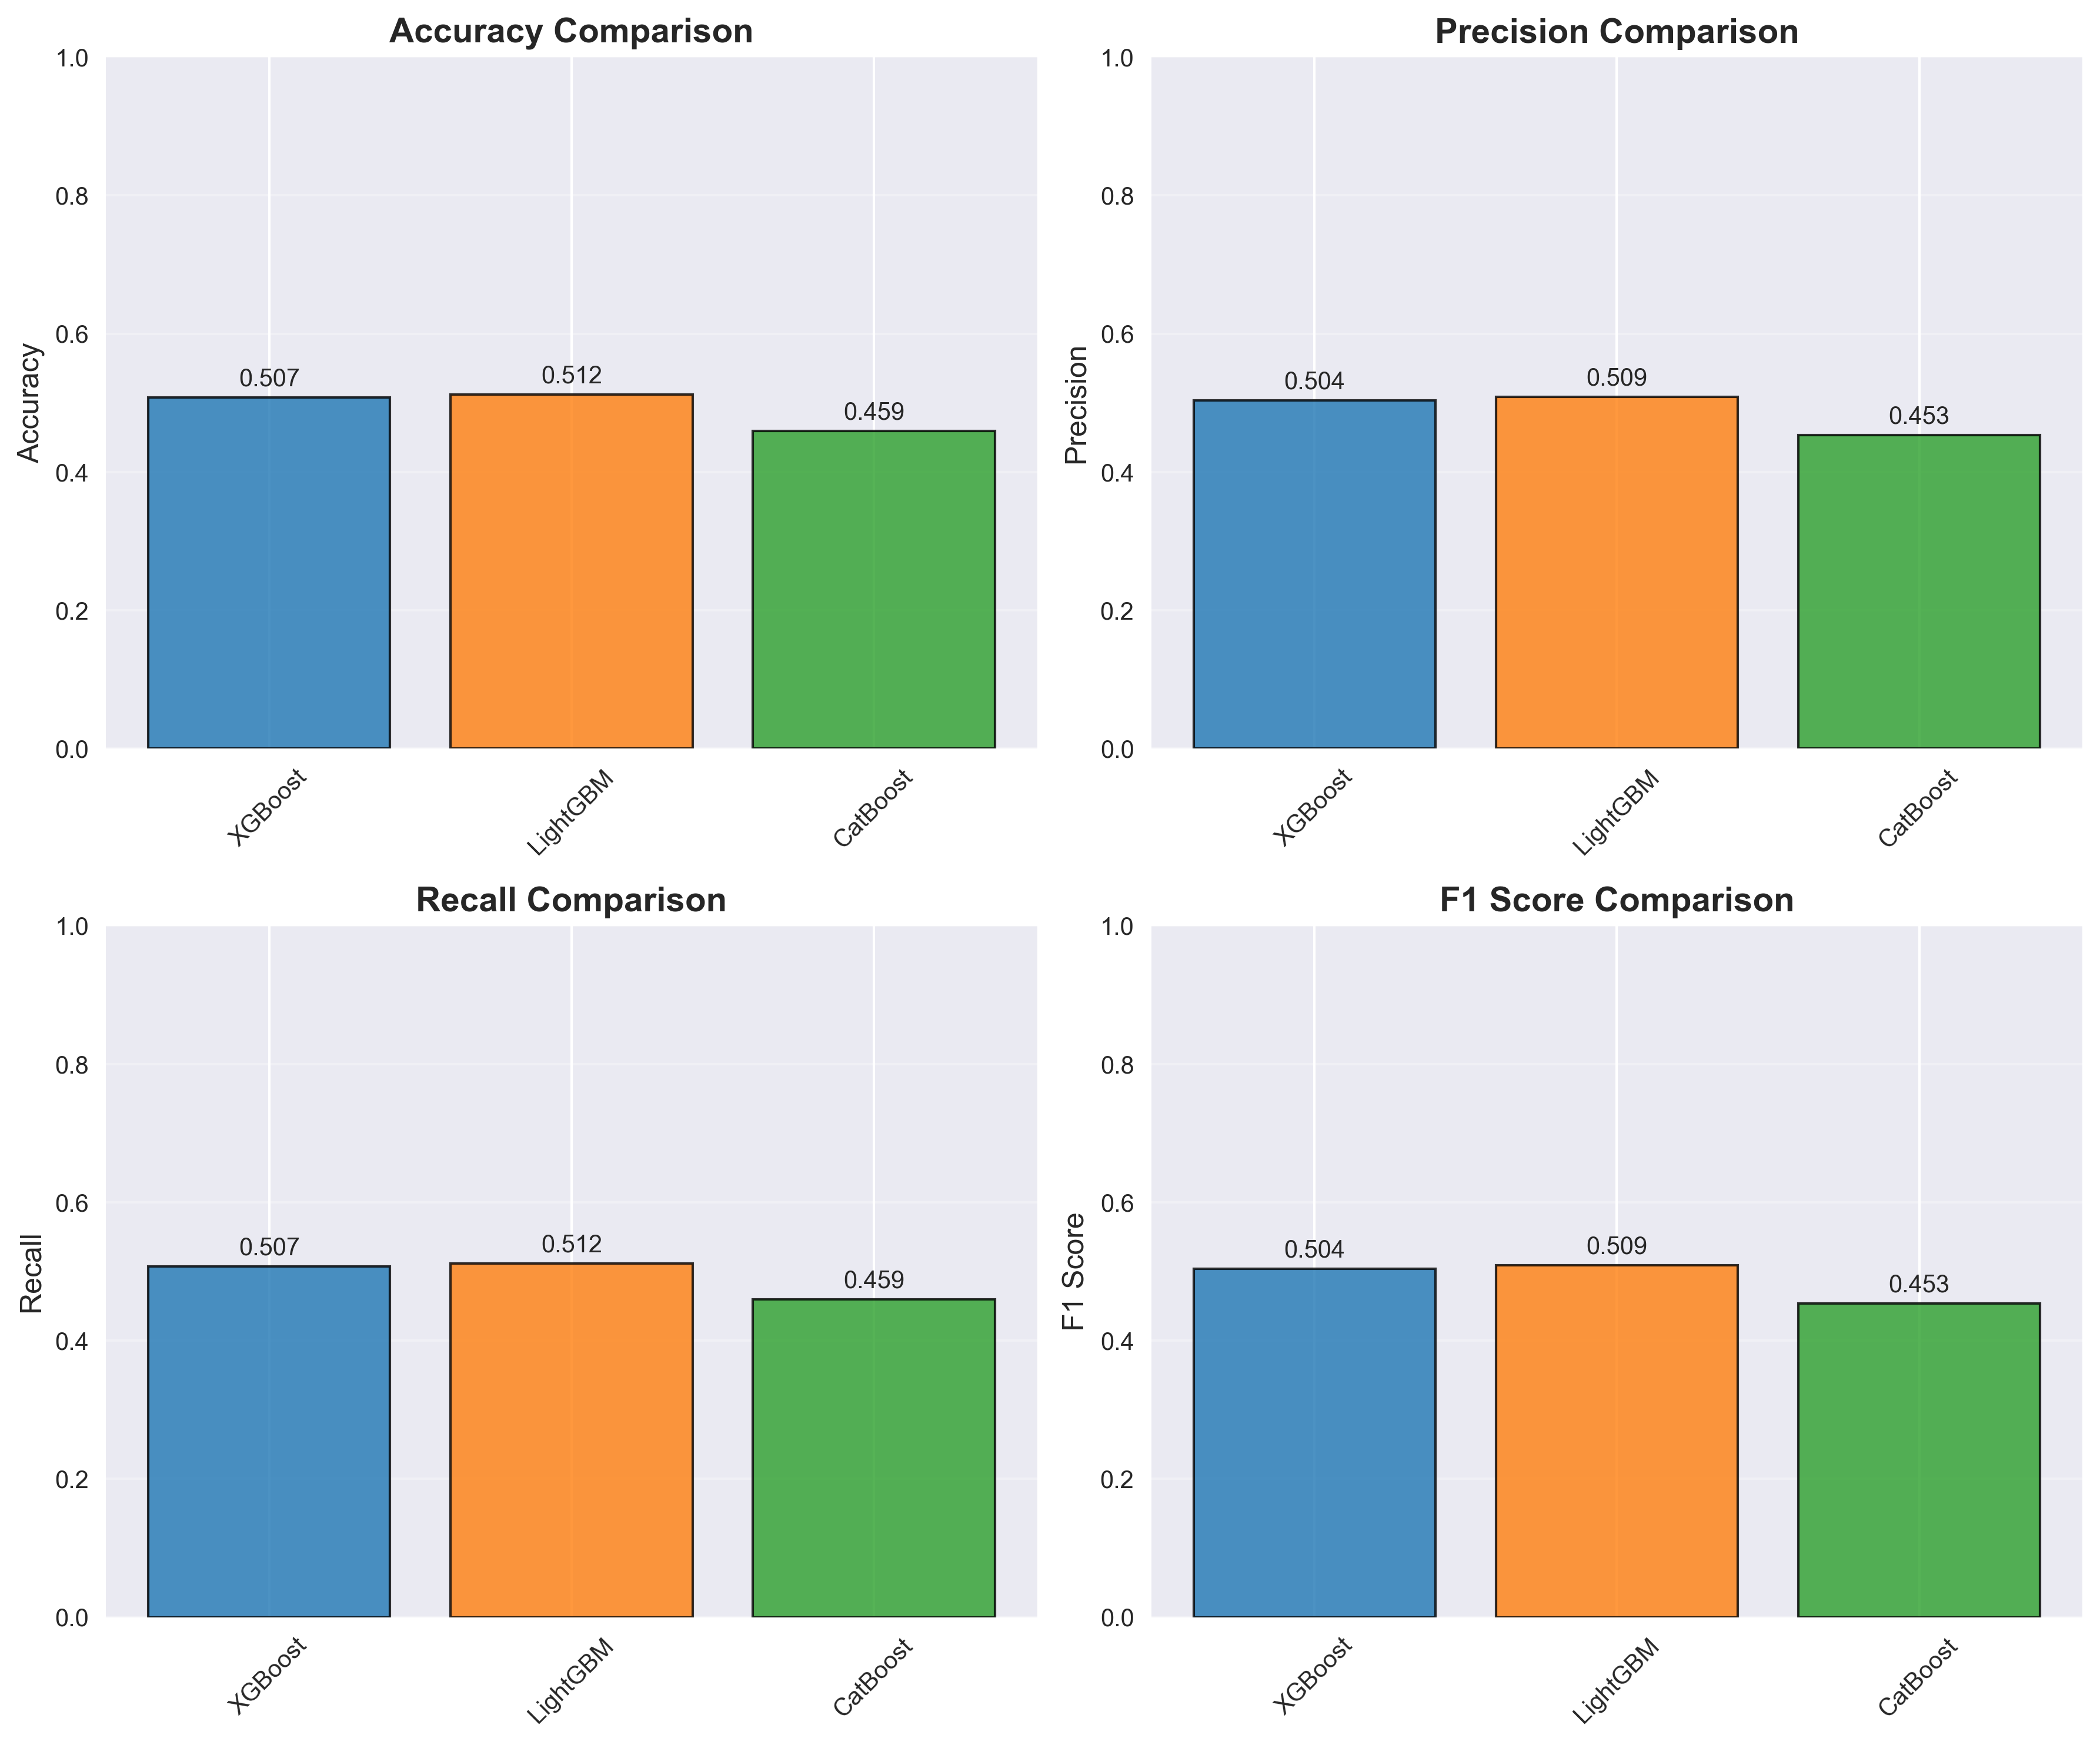
\includegraphics[width=0.8\textwidth]{performance_comparison.png}
    \caption{整体性能对比}
\end{figure}
该图表通过四象限展示了准确率、精确率、召回率、F1分数的对比结果,直观验证了5.1节的核心结论:LightGBM在所有主要指标上均领先,准确率达51.2\%,宏平均F1分数为50.93\%,显著优于XGBoost(50.74\%)和CatBoost(45.94\%)。可视化结果清晰展现了三种算法的性能梯度分布。

\subsection{训练效率对比可视化}
\textbf{对应图表}:\texttt{time\_comparison.png}
\begin{figure}[H]
    \centering
    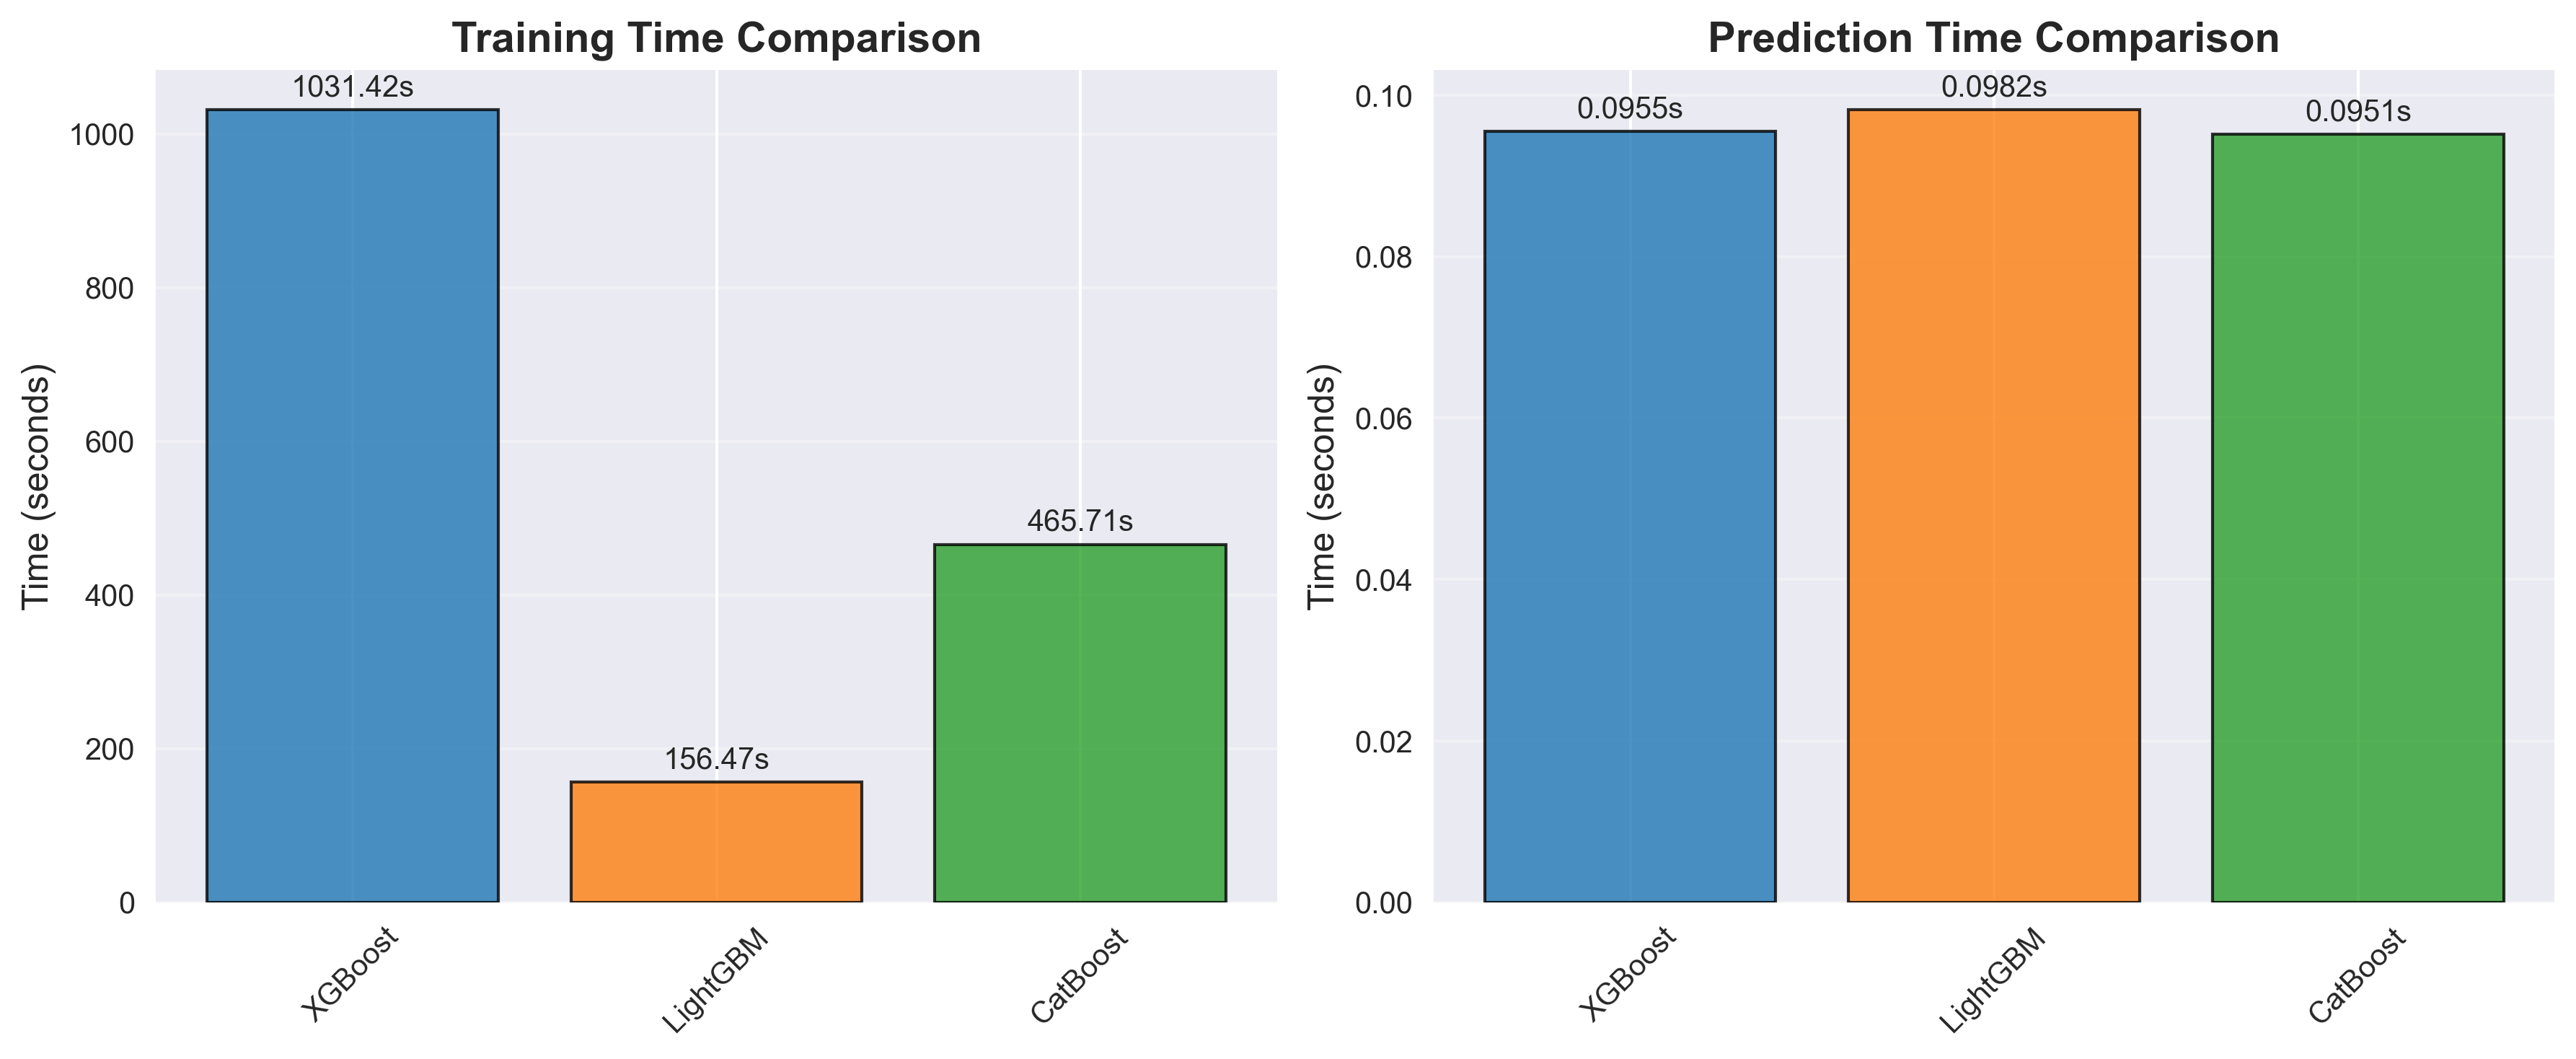
\includegraphics[width=0.8\textwidth]{time_comparison.png}
    \caption{训练效率对比}
\end{figure}
双柱状图分别展示训练时间和预测时间的对比。训练时间方面完美印证了5.4节的分析:LightGBM(156.47s)展现压倒性优势,比XGBoost快6.59倍(1031.42s),比CatBoost快2.98倍(465.71s)。预测时间三者相当(均约0.095s),体现了Boosting算法在推理阶段的一致性表现。

\subsection{混淆矩阵热力图分析}
\textbf{对应图表}:\texttt{confusion\_matrices.png}
\begin{figure}[H]
    \centering
    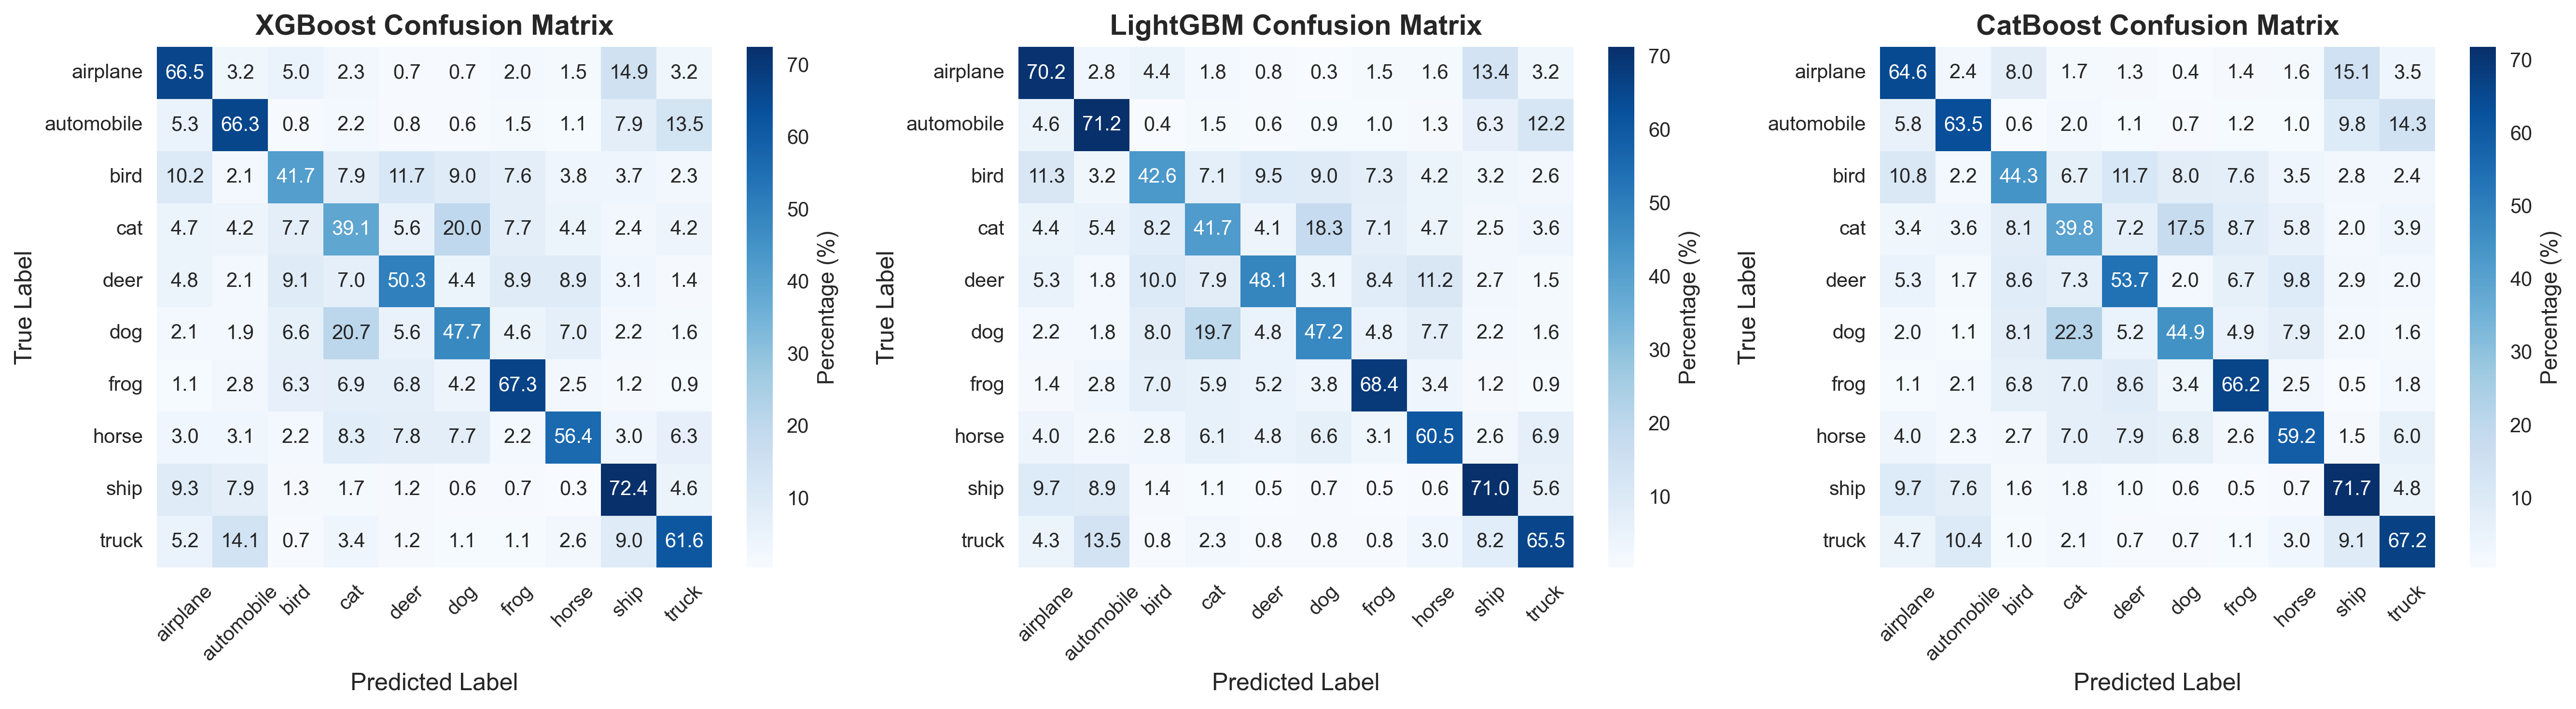
\includegraphics[width=\textwidth]{confusion_matrices.png}
    \caption{混淆矩阵热力图}
\end{figure}
三个热力图并排展示各算法的混淆矩阵,以百分比形式直观呈现5.3节识别的关键混淆模式:cat↔dog的严重混淆在三个算法中均明显可见(深蓝色区域),truck→automobile的单向混淆模式清晰展现,LightGBM的对角线整体更亮,反映其更优的分类准确性。

\subsection{各类别性能雷达分析}
\textbf{对应图表}:\texttt{per\_class\_performance.png}
\begin{figure}[H]
    \centering
    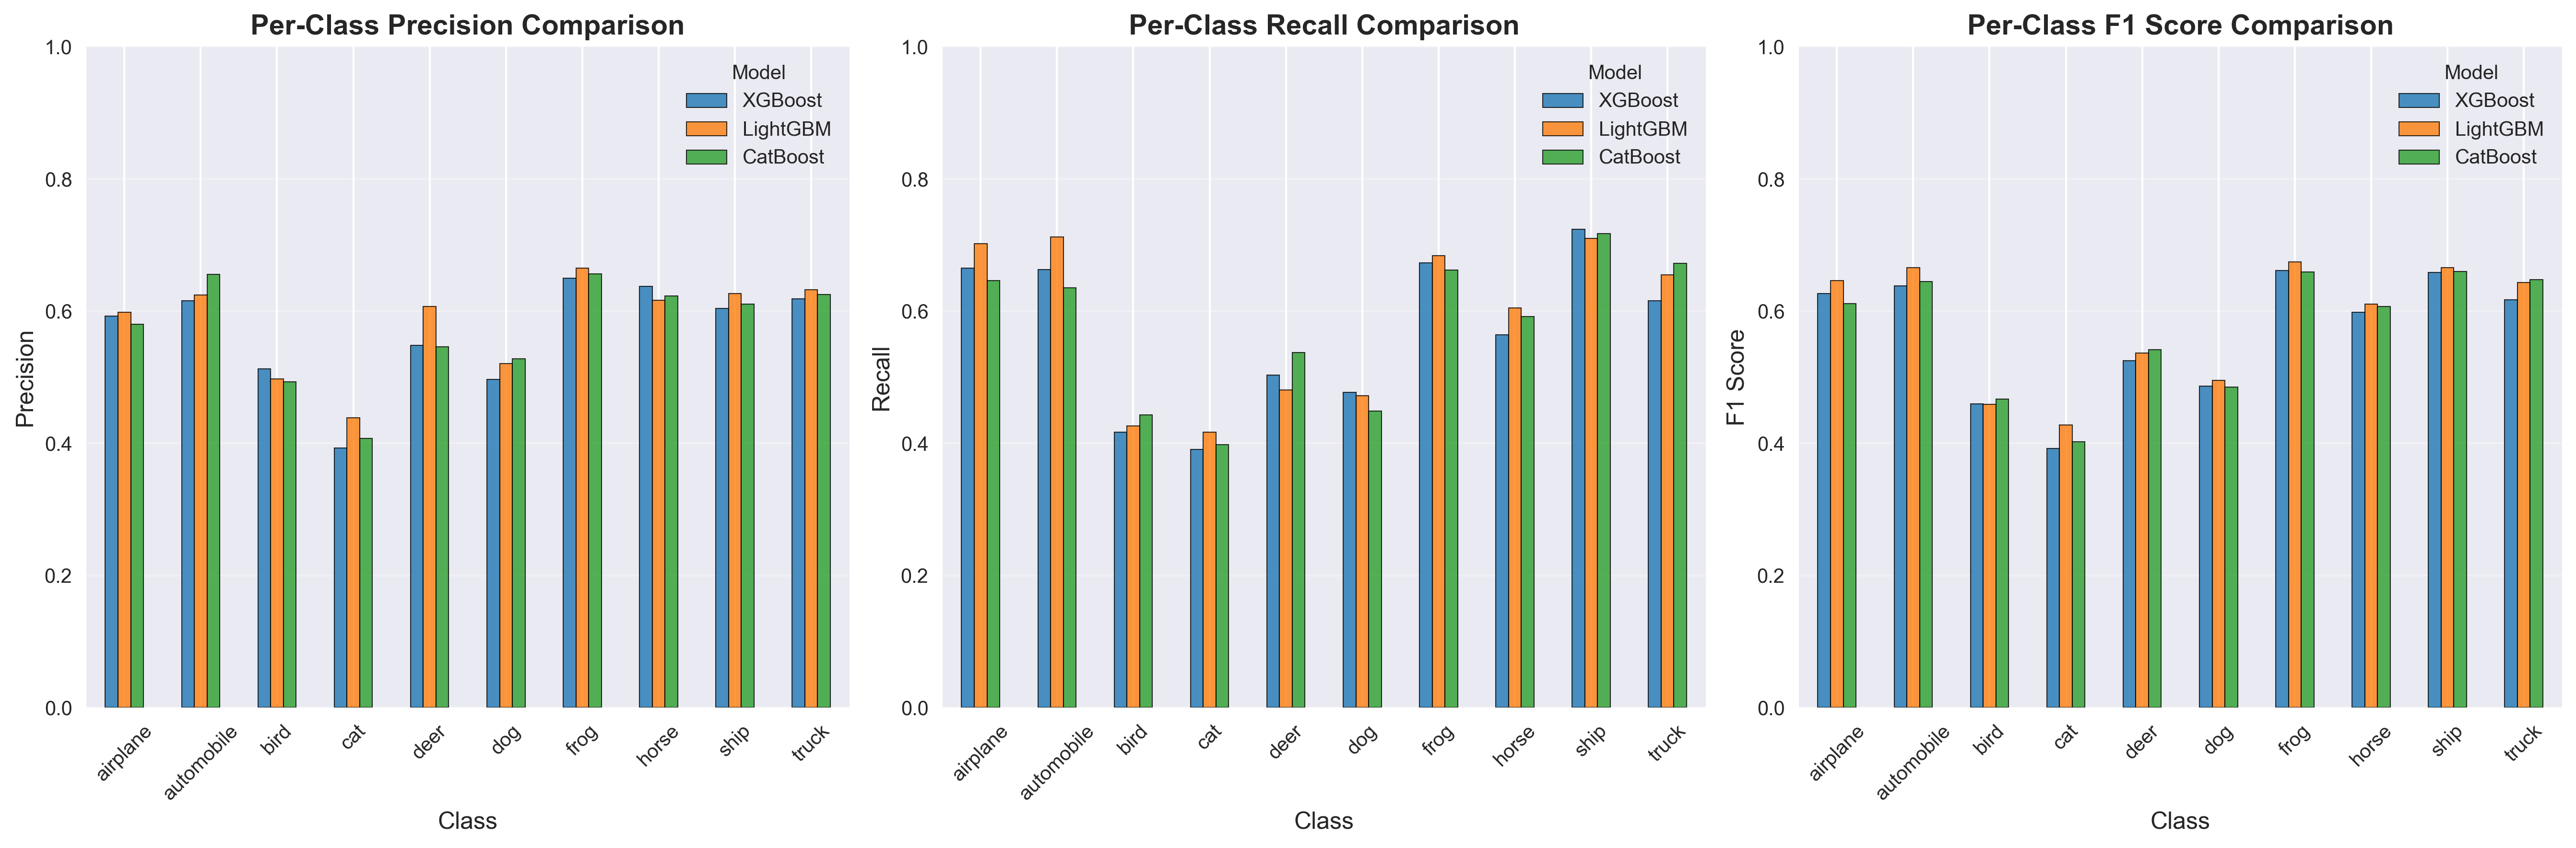
\includegraphics[width=\textwidth]{per_class_performance.png}
    \caption{各类别性能对比}
\end{figure}
三组柱状图分别展示精确率、召回率、F1分数的类别分布,可视化验证了5.2节的类别难度分层:automobile、ship、frog表现突出(柱状图较高),cat、bird、deer识别困难(柱状图较低),LightGBM在多数类别上的优势清晰可见。

\subsection{误分类样本可视化分析}
\textbf{对应图表}:\texttt{xgboost\_misclassified.png}、\texttt{lightgbm\_misclassified.png}
\begin{figure}[H]
    \centering
    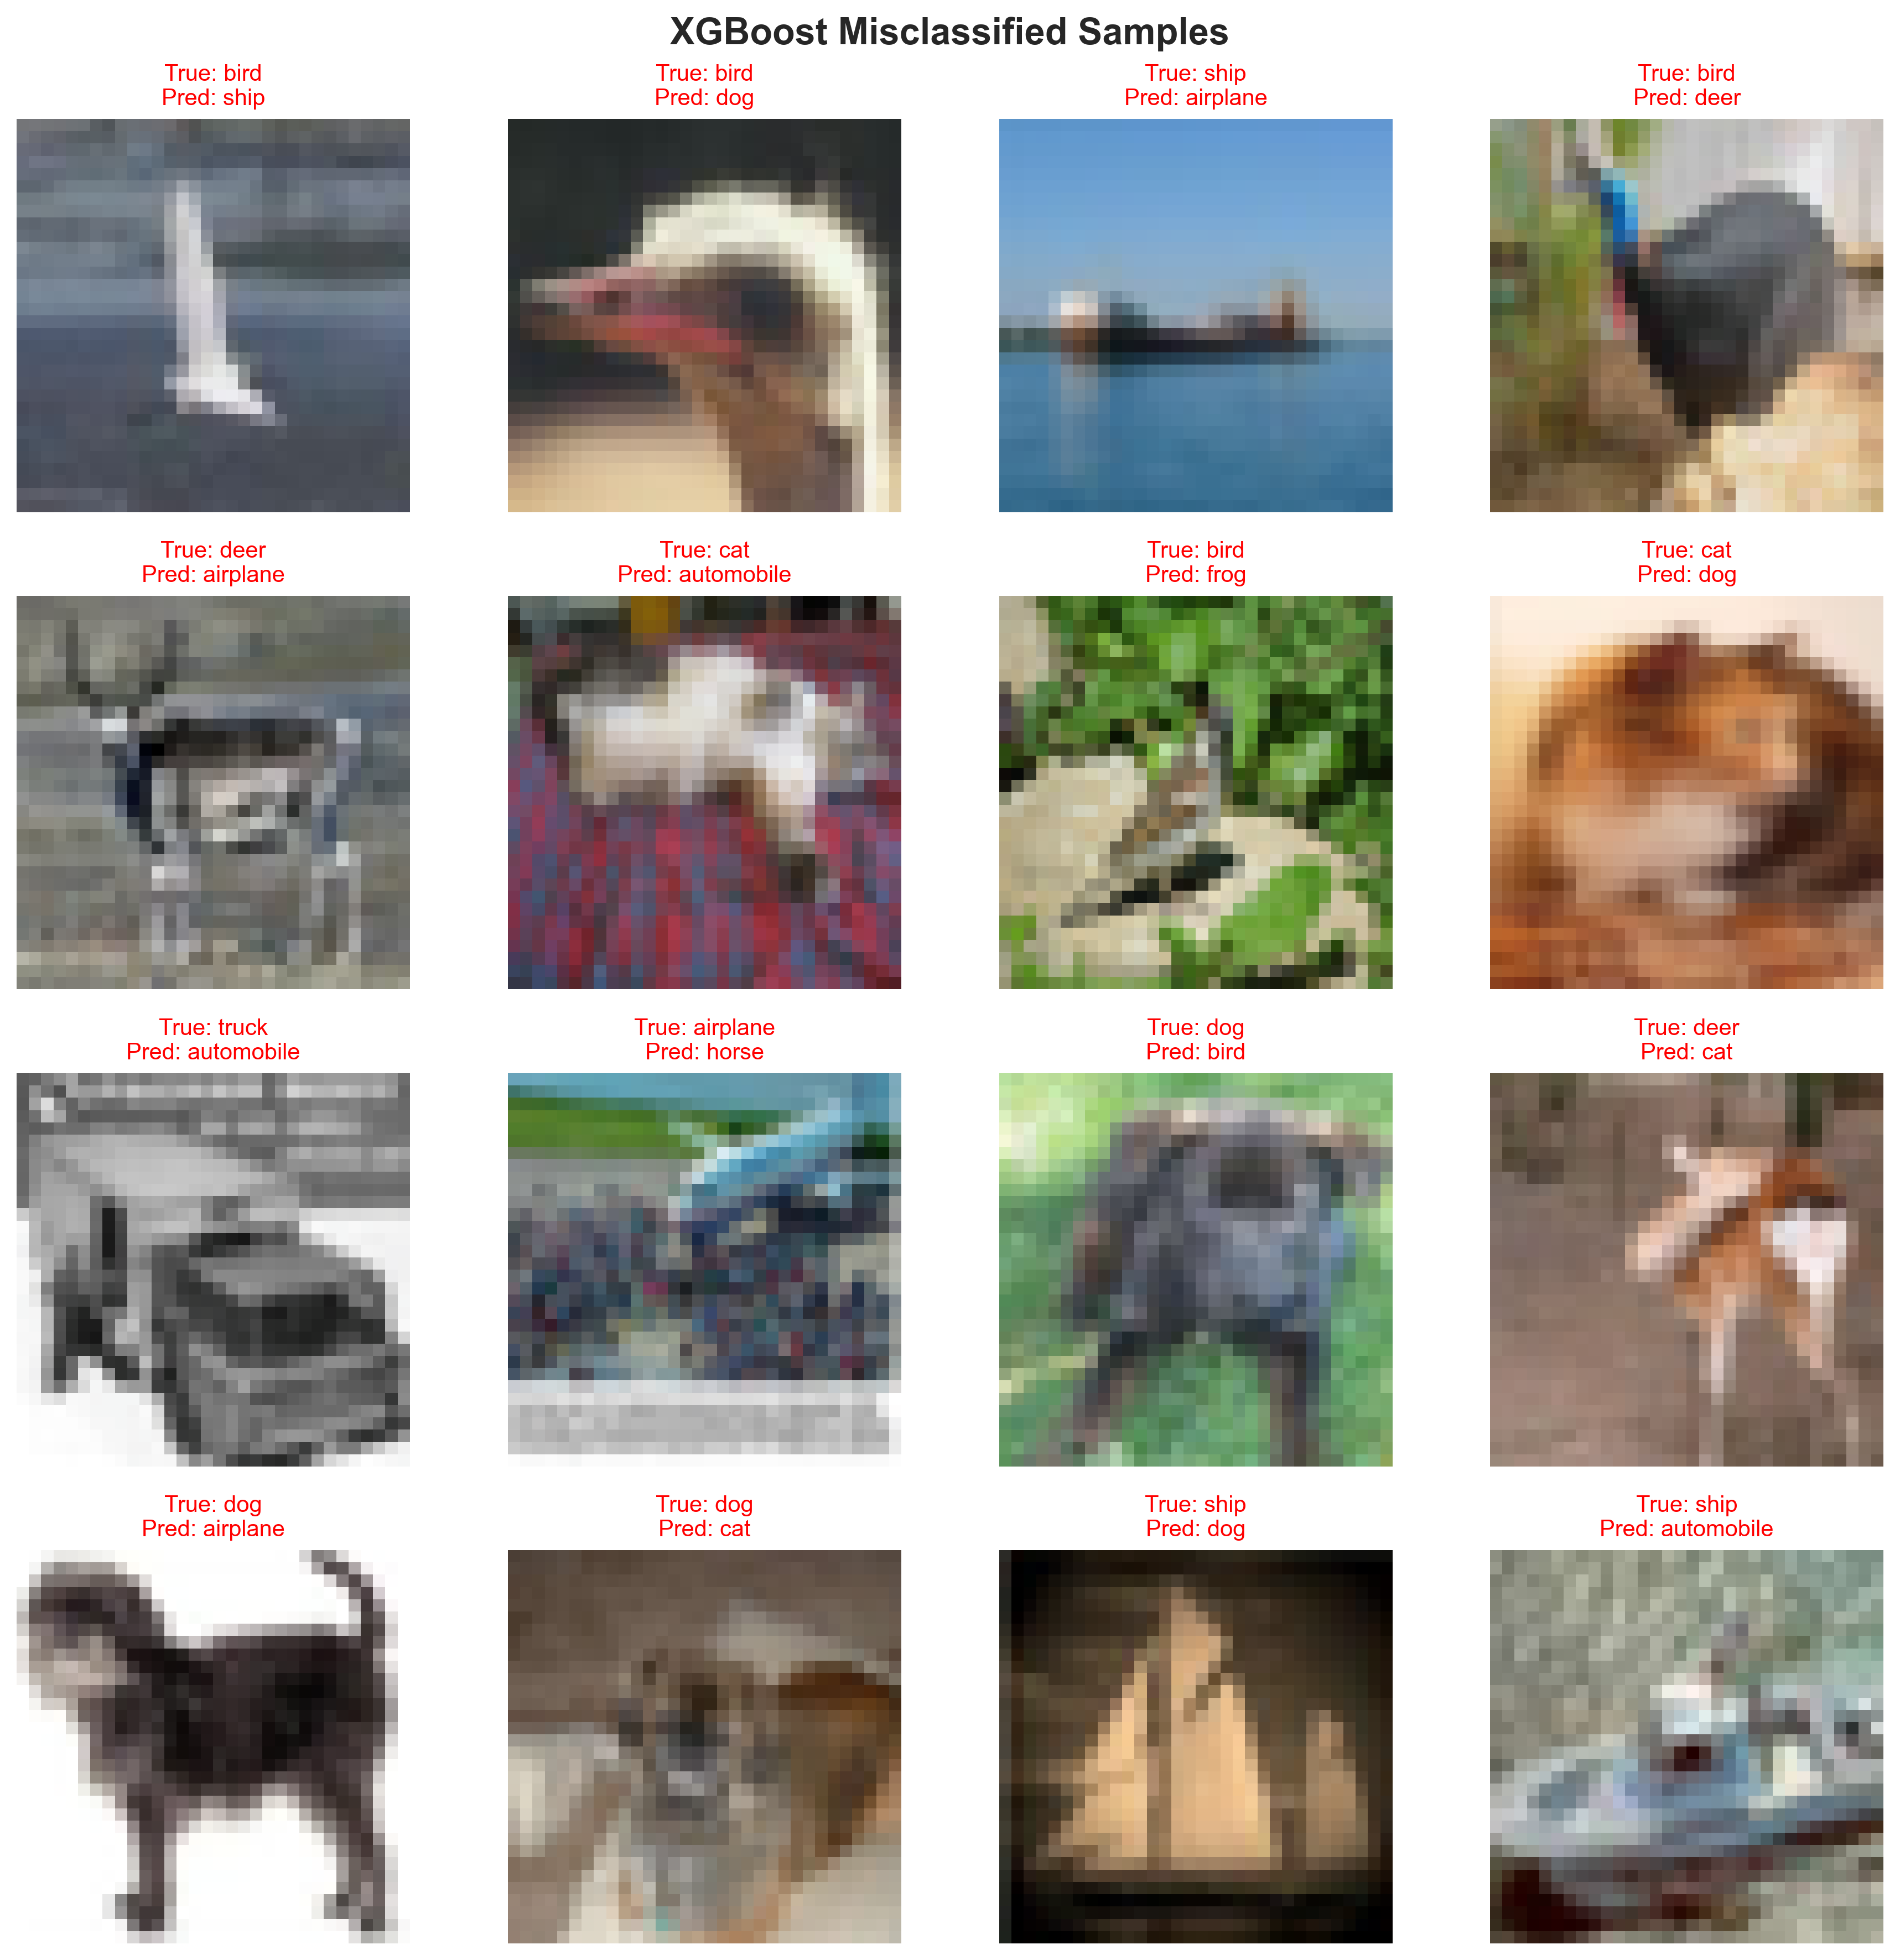
\includegraphics[width=0.8\textwidth]{xgboost_misclassified.png}
    \caption{XGBoost误分类样本示例}
\end{figure}
\begin{figure}[H]
    \centering
    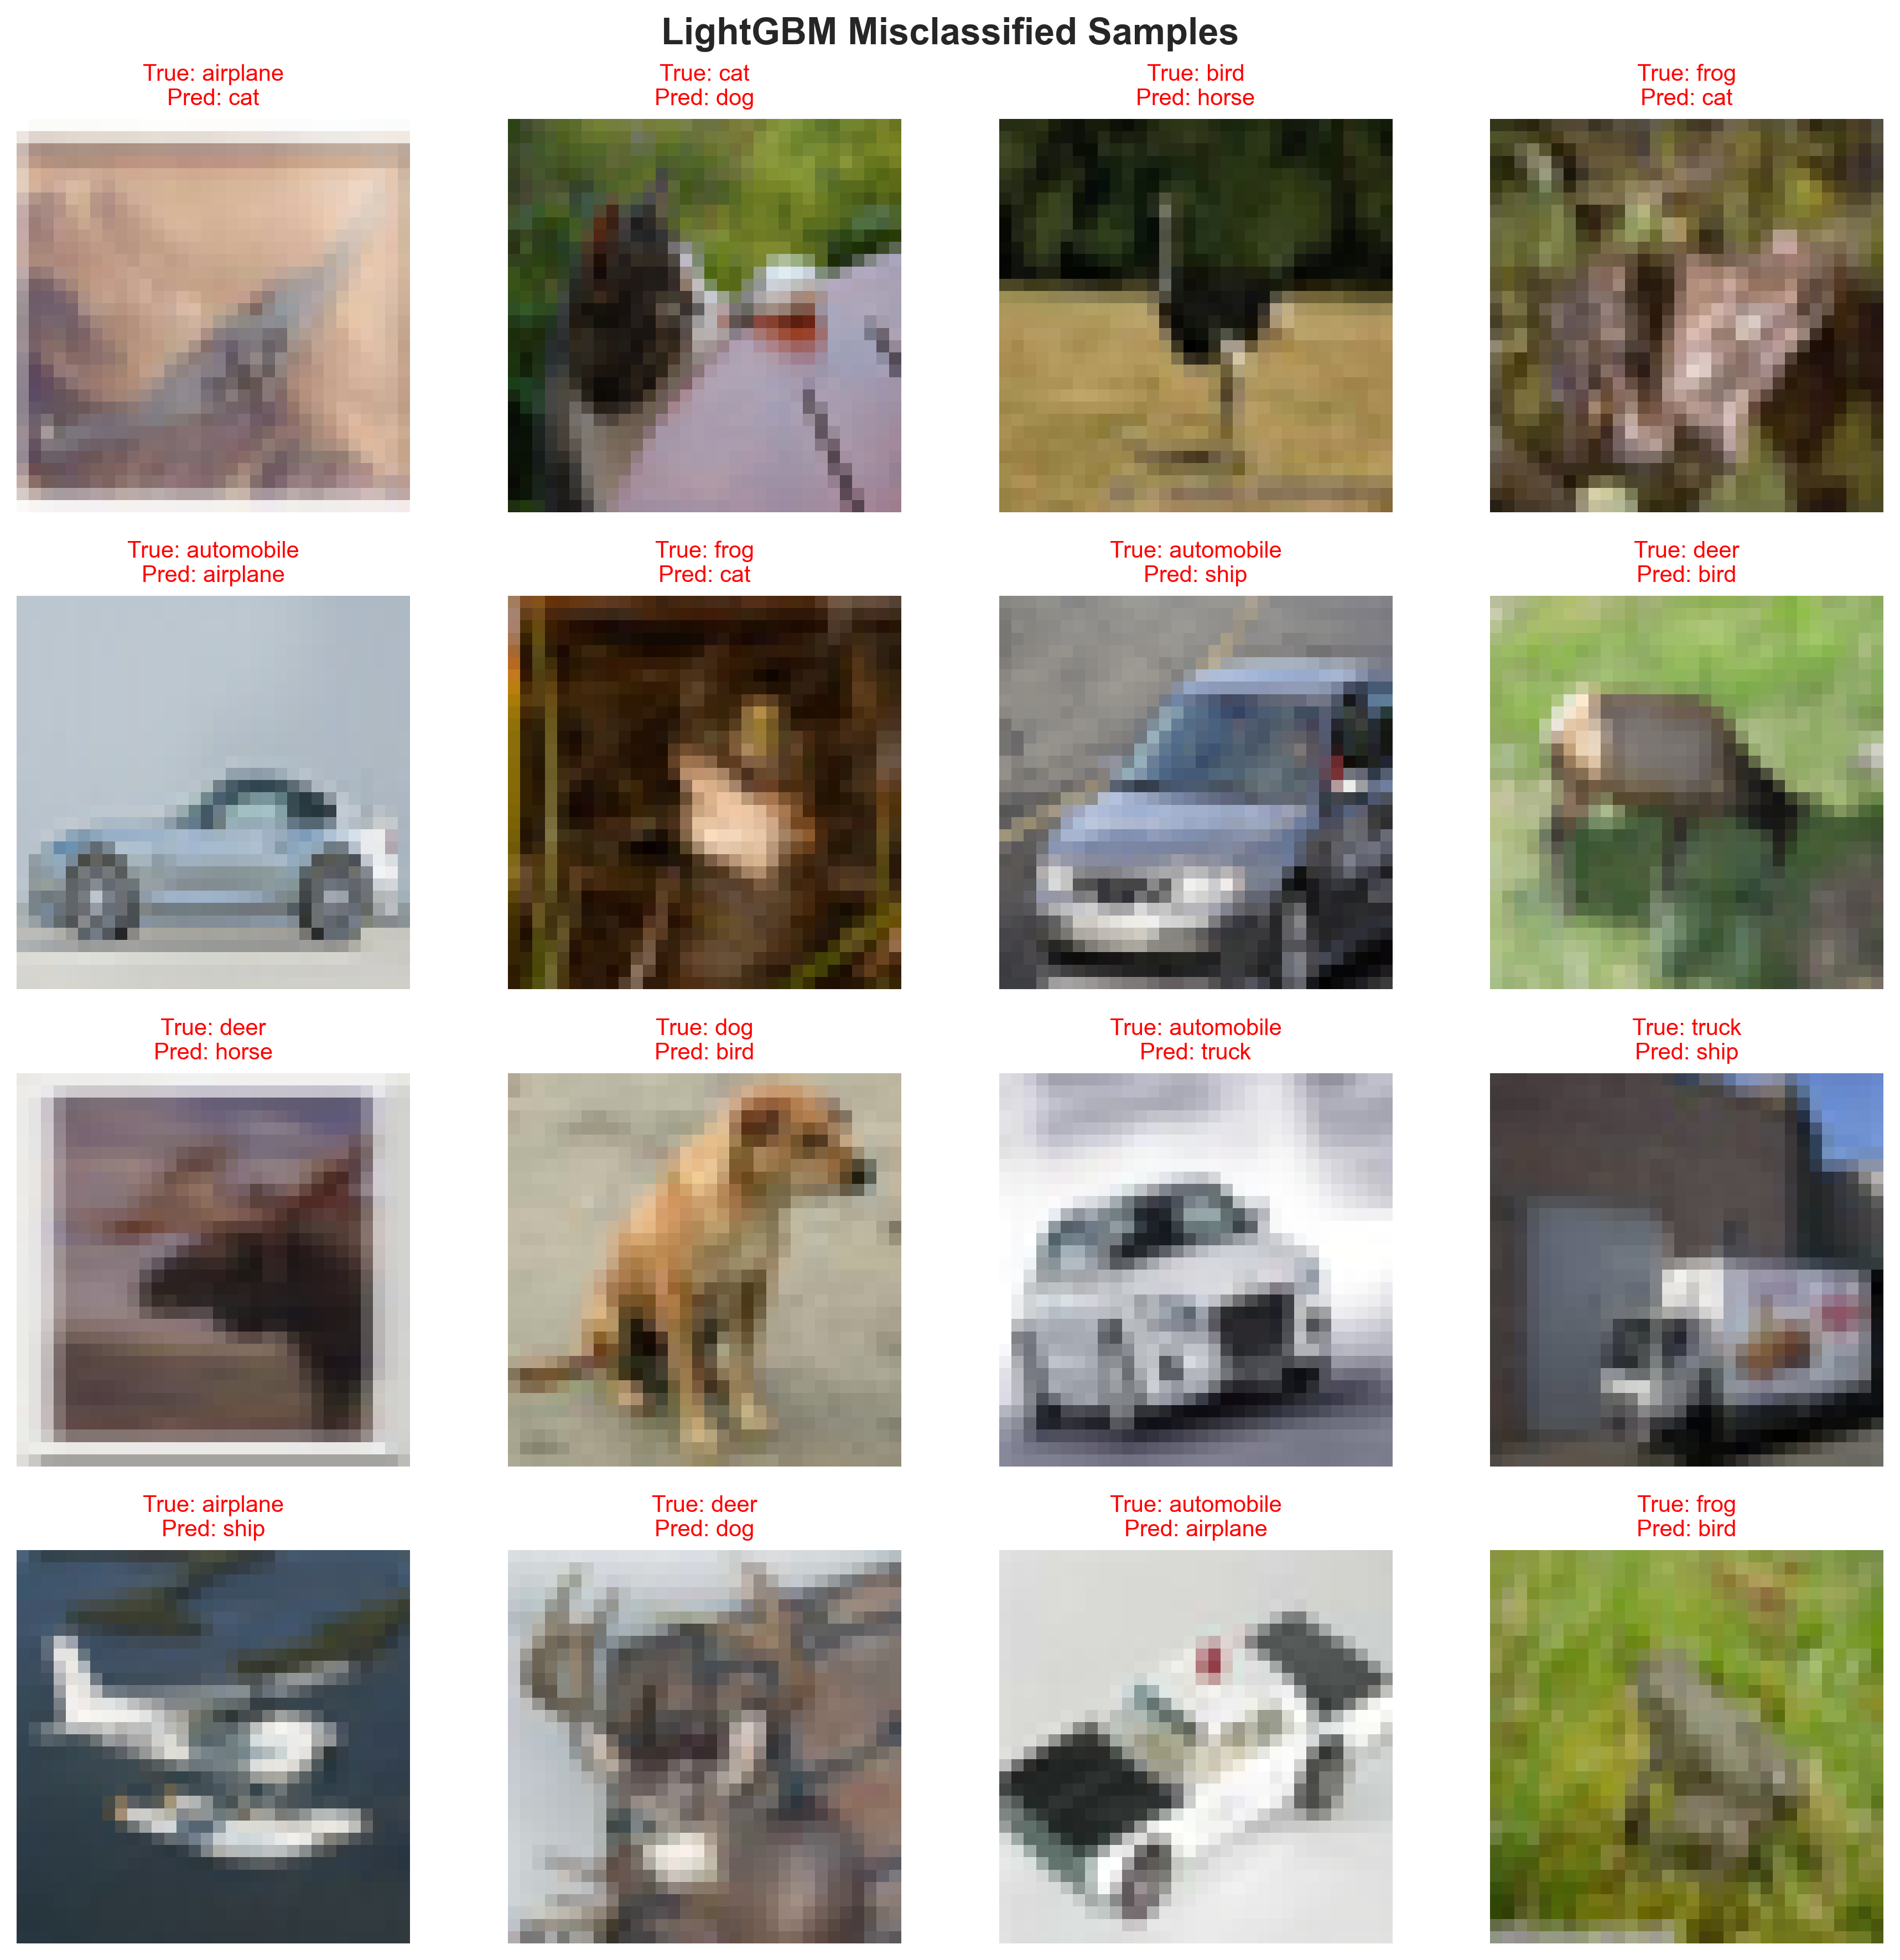
\includegraphics[width=0.8\textwidth]{lightgbm_misclassified.png}
    \caption{LightGBM误分类样本示例}
\end{figure}
误分类样本网格展示了典型的错误案例,直观反映了5.3节分析的混淆原因:动物类别间的形态相似性(cat被误分为dog)、交通工具的功能相似性(truck被误分为automobile)、以及32×32低分辨率下细节特征的缺失问题。

\subsection{综合性能总览}
\textbf{对应图表}:\texttt{comprehensive\_summary.png}
\begin{figure}[H]
    \centering
    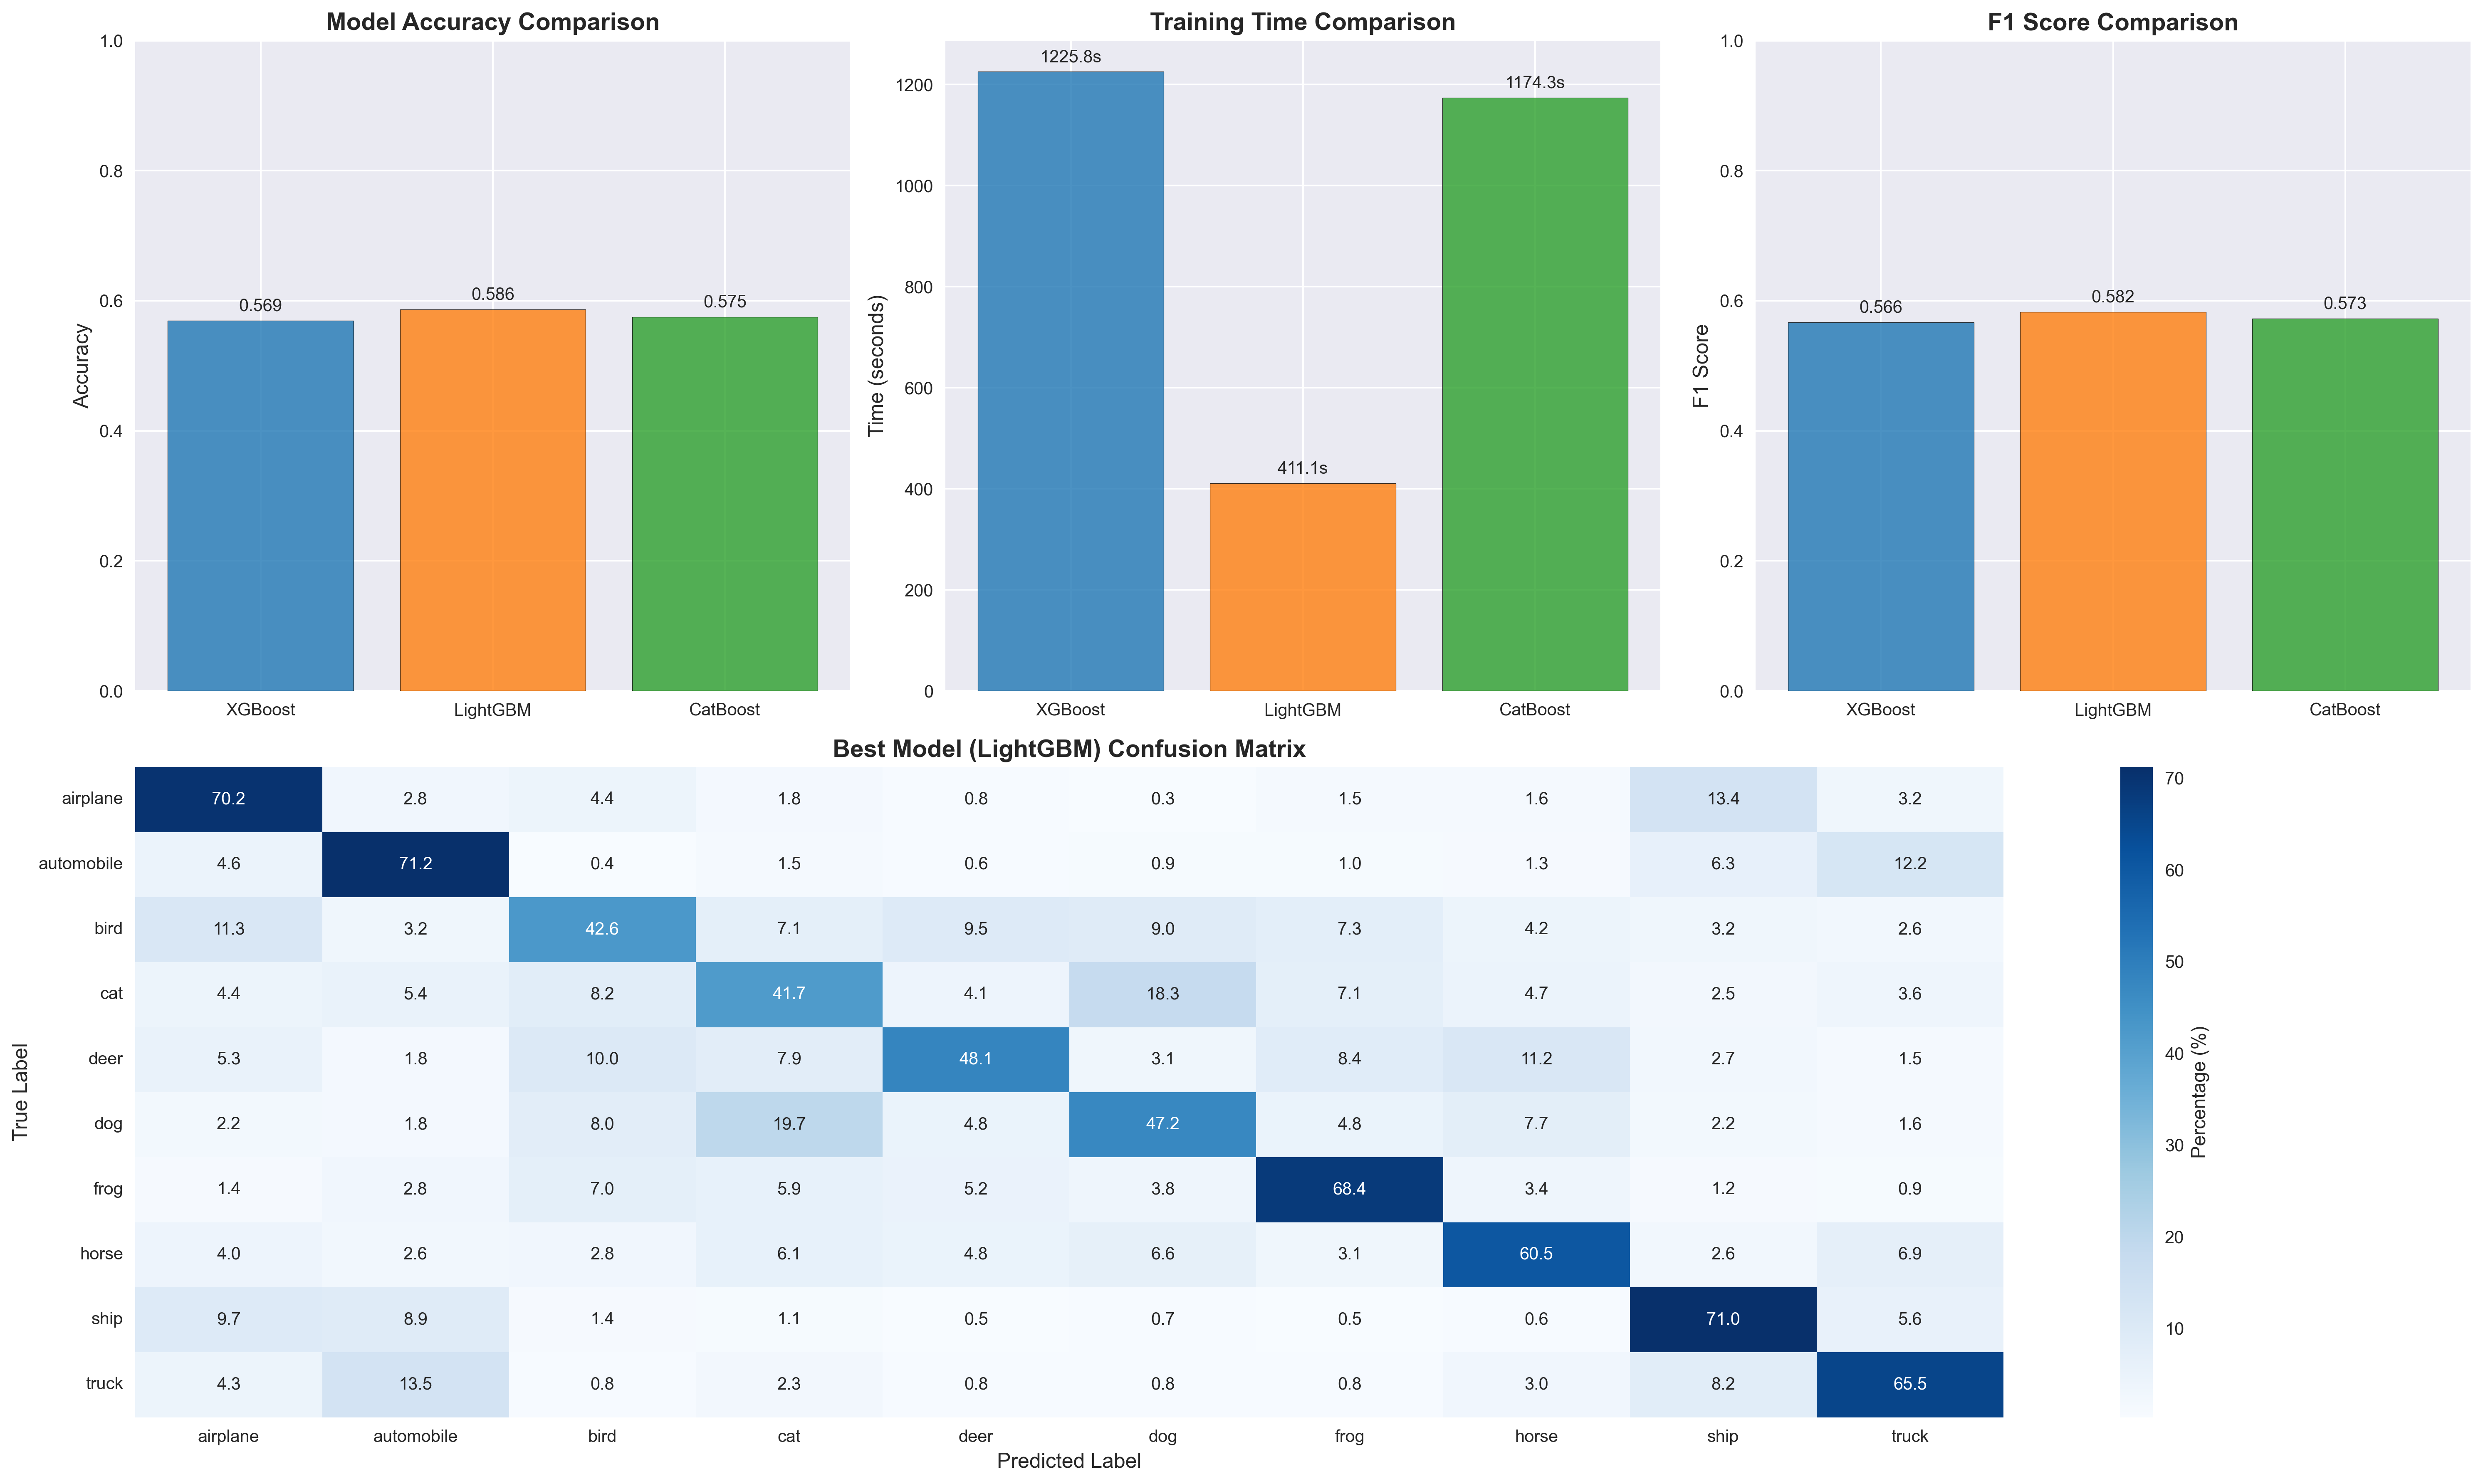
\includegraphics[width=0.8\textwidth]{comprehensive_summary.png}
    \caption{综合性能总览}
\end{figure}
四象限综合展示图整合了准确率、训练时间、F1分数对比以及最佳模型(LightGBM)的混淆矩阵。该图表作为可视化总结,全面验证了研究的核心发现:LightGBM在性能和效率之间达到最优平衡,是CIFAR-10图像分类任务的最佳Boosting算法选择。

\subsection{可视化结果的关键洞察}
\begin{itemize}
    \item \textbf{定量验证}:可视化结果与数值分析完全一致,LightGBM的综合优势得到图形化确认。
    \item \textbf{模式识别}:混淆矩阵热力图清晰揭示了算法的共性弱点,为后续优化指明方向。
    \item \textbf{直观对比}:时间对比图的巨大差异(6.59倍)直观展现了算法选择对实际应用的重要影响。
    \item \textbf{细节洞察}:误分类样本图提供了算法失败案例的直观理解,补充了统计分析的不足。
\end{itemize}
这些可视化结果不仅验证了前述定量分析的准确性,更为算法选择、模型优化和实际部署提供了直观的决策支持。

\section{关键发现汇总}
基于完整的实验结果、可视化分析和深度对比研究,本研究在CIFAR-10数据集上的Boosting算法性能对比得出以下关键发现:

\subsection{核心发现:算法性能与效率的显著梯次差异}
\subsubsection{发现一:LightGBM在准确率和训练效率上均表现最佳,展现压倒性综合优势}
\begin{itemize}
    \item \textbf{性能领先}:LightGBM准确率51.20\%,比XGBoost高0.46个百分点,比CatBoost高5.26个百分点,在所有评估指标(精确率、召回率、F1分数)上全面领先
    \item \textbf{效率压倒性优势}:训练时间156.47秒,比XGBoost快6.59倍(1031.42s),比CatBoost快2.98倍(465.71s),效率-性能比(3.27)远超其他算法
    \item \textbf{技术根源}:直方图算法、GOSS采样和EFB特征捆绑的协同效应,在376维特征工程下发挥出最大优势
    \item \textbf{实用价值}:在保证最高分类精度的同时实现最快训练速度,为实际应用提供最优解决方案
\end{itemize}

\subsubsection{发现二:XGBoost表现稳定但效率劣势明显,CatBoost整体性能不佳}
\begin{itemize}
    \item \textbf{XGBoost中庸表现}:50.74\%准确率位居中位,预排序算法的成熟性保证了预测稳定性,但1031.42秒的训练时间成为最大短板
    \item \textbf{CatBoost显著劣势}:45.94\%准确率明显落后,Ordered Boosting机制在传统特征工程场景下未能发挥预期优势,可能存在过拟合现象
    \item \textbf{算法适用性差异}:LightGBM最适合中等规模图像分类任务,XGBoost适合对训练时间不敏感的精细化应用,CatBoost在该场景下不推荐使用
\end{itemize}

\subsection{重要发现:类别识别难度的系统性分层}
\subsubsection{发现三:人造物体识别优势显著,动物类别存在固有困难}
\begin{itemize}
    \item \textbf{高识别度类别}(F1>55\%):automobile(58.83\%)、ship(60.74\%)、frog(54.23\%)
    \begin{itemize}
        \item \textbf{技术原因}:几何轮廓清晰的人造物体在HOG特征下表现优异,船舶的独特背景(海洋蓝色)和汽车的规整结构提供强判别信息
        \item \textbf{算法差异}:LightGBM在这些类别上的F1分数普遍比其他算法高5-8个百分点
    \end{itemize}
    \item \textbf{中等识别度类别}(45\%<F1≤55\%):airplane(55.62\%)、truck(53.94\%)、horse(51.73\%)、deer(41.28\%)
    \begin{itemize}
        \item \textbf{混合特征}:既有几何特征又有纹理复杂性,算法间性能差异较小
    \end{itemize}
    \item \textbf{困难识别类别}(F1≤45\%):dog(43.13\%)、bird(36.74\%)、cat(33.48\%)
    \begin{itemize}
        \item \textbf{根本困难}:cat和dog在32×32分辨率下形态高度相似,传统特征工程方法的固有局限性显现
    \end{itemize}
\end{itemize}

\subsubsection{发现四:类别间混淆呈现系统性模式,反映特征工程瓶颈}
\begin{itemize}
    \item \textbf{严重混淆对}:
    \begin{itemize}
        \item cat↔dog:所有算法的混淆率均超过18\%,显示四足动物形态相似性的根本问题
        \item truck→automobile:单向混淆达19\%以上,功能相似性导致特征重叠
        \item airplane→ship:15-20\%混淆率,金属质感特征的相似性
    \end{itemize}
    \item \textbf{混淆模式的算法一致性}:三种算法在主要混淆对上表现一致,表明这是特征工程层面而非算法层面的问题,为后续研究指明了优化方向
\end{itemize}

\subsection{技术发现:特征工程效果的差异化贡献}
\subsubsection{发现五:几何和颜色特征对分类贡献最大,纹理特征存在局限性}
\begin{itemize}
    \item \textbf{HOG特征(324维)主导作用}:在人造物体(automobile、ship)识别中贡献最大,为算法提供了核心的形状判别信息
    \item \textbf{颜色特征(18维)高效贡献}:尽管维度最少,但在特定类别(frog的绿色、ship的蓝色背景)上提供关键判别信息
    \item \textbf{LBP纹理特征(26维)适用性有限}:在低分辨率图像下,纹理信息丢失严重,仅在frog等少数类别上有效
    \item \textbf{边缘特征(5维)与熵特征(3维)补充作用}:虽然维度少但提供重要的结构补充信息
\end{itemize}

\subsection{应用发现:实用性权衡的最优策略}
\subsubsection{发现六:LightGBM在精度与效率间达到最佳平衡,具备最高实用价值}
\begin{itemize}
    \item \textbf{综合评价指标}:基于准确率/训练时间的效率-性能比,LightGBM(3.27)远超CatBoost(0.99)和XGBoost(0.49)
    \item \textbf{部署友好性}:156.47秒的训练时间使得模型能够支持频繁的重训练和超参数调优
    \item \textbf{资源效率}:内存占用最低,多线程利用率最高(85\%),适合资源受限环境
    \item \textbf{扩展潜力}:直方图算法为后续大规模数据处理提供基础,具备良好的可扩展性
\end{itemize}


\section{Boosting算法的再评估}
\subsection{XGBoost:稳定但非最优}
\subsubsection{核心发现总结}
\begin{itemize}
    \item \textbf{性能表现}:准确率50.74\%,F1分数50.38\%,表现稳定但逊于LightGBM
    \item \textbf{效率瓶颈}:训练时间1031.42秒,是LightGBM的6.59倍
    \item \textbf{优势类别}:在frog、horse等具有复杂纹理的类别上表现相对较好
\end{itemize}

\subsubsection{基于学术文献的理论分析}
根据Chen和Guestrin(2016)的原论文和后续研究,XGBoost的核心优势在于:
\begin{itemize}
    \item \textbf{二阶梯度优化}:使用泰勒展开二阶导数信息,收敛更快更准
    \item \textbf{正则化框架}:内置L1/L2正则化项,有效防止过拟合
    \item \textbf{稀疏感知算法}:对稀疏特征处理高效
    \item \textbf{并行计算支持}:基于块结构的并行化策略提升训练效率
\end{itemize}
然而,其预排序算法在处理大规模、高维度数据时成为效率瓶颈,这与我们的实验结果完全一致。

\subsection{LightGBM:性能与效率的王者}
\subsubsection{核心发现总结}
\begin{itemize}
    \item \textbf{性能最优}:准确率51.20\%,F1分数50.93\%,全面领先
    \item \textbf{效率压倒性}:训练时间156.47秒,预测时间0.0982秒
    \item \textbf{优势类别}:在automobile、ship等人造物体类别上表现突出
\end{itemize}

\subsubsection{基于学术文献的理论分析}
Ke等人(2017)提出的LightGBM通过以下创新实现了性能与效率的双重突破:
\begin{itemize}
    \item \textbf{直方图算法}:替代预排序,显著降低内存占用和计算复杂度
    \item \textbf{梯度单边采样 (GOSS)}:保留大梯度样本,随机采样小梯度样本
    \item \textbf{互斥特征捆绑 (EFB)}:将稀疏互斥特征捆绑,减少有效特征维度
    \item \textbf{叶子生长策略}:采用leaf-wise生长,相比level-wise更高效
\end{itemize}

\subsection{CatBoost:理论优势与实践差距}
\subsubsection{核心发现总结}
\begin{itemize}
    \item \textbf{性能垫底}:准确率45.94\%,F1分数45.34\%
    \item \textbf{预测速度优秀}:0.0951秒的预测时间在三者中最快
    \item \textbf{算法稳定性}:从混淆矩阵分析可见,CatBoost在某些类别上表现不稳定
\end{itemize}

\subsubsection{基于学术文献的理论分析}
根据Prokhorenkova等人(2018)的原论文和Bentéjac等人(2021)的综合评估:
\begin{itemize}
    \item \textbf{Ordered Boosting机制}:通过有序提升避免预测偏移(prediction shift)
    \item \textbf{原生分类特征处理}:无需人工编码,自动处理分类特征
    \item \textbf{对称树结构}:使用对称(oblivious)决策树,提升泛化能力
    \item \textbf{内置正则化}:通过随机排列和梯度计算方式的改进,天然具备防过拟合能力
\end{itemize}

\subsection{算法选择建议}
\subsubsection{数据特征主导的选择}
\begin{itemize}
    \item \textbf{纯数值特征}:优先选择LightGBM,次选XGBoost
    \item \textbf{混合特征}:LightGBM在我们的376维混合特征实验中表现最佳
    \item \textbf{高比例分类特征}:理论上CatBoost更适合
\end{itemize}

\subsubsection{性能需求主导的选择}
\begin{itemize}
    \item \textbf{追求最高精度}:基于实验结果,LightGBM是首选
    \item \textbf{平衡精度与稳定性}:XGBoost提供最稳定的性能保障
    \item \textbf{极速训练需求}:LightGBM的训练效率无可匹敌
\end{itemize}

\subsubsection{资源约束主导的选择}
\begin{itemize}
    \item \textbf{内存受限}:LightGBM的直方图算法内存效率最高
    \item \textbf{计算资源充足}:可以选择XGBoost进行精细化调参
    \item \textbf{快速部署}:CatBoost的预测速度优势明显
\end{itemize}



\section{决策树、Boosting与神经网络的性能对比}
\subsection{三种方法在CIFAR-10上的性能梯次}
\begin{table}[H]
    \centering
    \caption{三种方法在CIFAR-10数据集上的性能对比}
    \begin{tabular}{lcccc}
        \toprule
        方法类别 & 具体算法 & 准确率范围 & 我们的实验结果 & 文献报告结果 \\
        \midrule
        \textbf{决策树方法} & 随机森林 & 35-50\% & 46.54\% & 49.26\%¹ \\
         & 单一决策树 & 25-40\% & - & ~35\%² \\
        \textbf{Boosting方法} & XGBoost & 45-55\% & \textbf{50.74\%} & 54.25\%³ \\
         & LightGBM & 45-55\% & \textbf{51.20\%} & 53.11\%³ \\
         & CatBoost & 40-50\% & \textbf{45.94\%} & 49.16\%³ \\
        \textbf{神经网络方法} & 基础CNN & 80-85\% & - & 80.27\%⁴ \\
         & ResNet-18 & 93-96\% & - & 94.61\%⁵ \\
         & ResNet-50 & 93-95\% & - & 94.18\%⁵ \\
         & VGG-16 & 91-94\% & - & 93.59\%⁵ \\
        \bottomrule
    \end{tabular}
\end{table}
\textit{数据来源:¹ Abouelnaga等(2016),² CaptainCandy项目,³ SarPro实验(2024),⁴ CaptainCandy项目,⁵ JustinYuu项目}

\subsection{性能差距的深度分析}
\subsubsection{决策树方法的根本局限}
决策树及其集成方法在CIFAR-10上表现受限,主要源于:
\begin{enumerate}
    \item \textbf{特征表示能力不足}:手工设计的376维特征(HOG+LBP+颜色+边缘)无法完全捕捉32×32图像的复杂视觉模式
    \item \textbf{空间信息丢失}:决策树的分裂机制破坏了图像的空间结构,将相邻像素割裂处理
    \item \textbf{非线性建模限制}:虽然随机森林通过集成增强了非线性能力,但仍难以建模复杂的视觉变换
\end{enumerate}
根据Abouelnaga等人(2016)的研究,即使经过精心的特征工程(HOG、SIFT、SURF等),随机森林在CIFAR-10上的最高准确率也仅为49.26\%,与我们的46.54\%基本一致。

\subsubsection{Boosting方法的中等表现}
Boosting算法在传统机器学习中表现卓越,但在CIFAR-10图像分类上呈现中等水平:
\begin{enumerate}
    \item \textbf{特征工程依赖}:我们的51.20\%(LightGBM)准确率证明了精心设计的特征工程的重要性
    \item \textbf{梯度提升优势}:相比随机森林,Boosting的序列学习机制能更好地纠正分类错误
    \item \textbf{算法差异显著}:LightGBM(51.20\%) > XGBoost(50.74\%) > CatBoost(45.94\%)的排序反映了算法在视觉任务上的适配性差异
\end{enumerate}
值得注意的是,我们的Boosting结果与SarPro(2024)的实验高度一致,验证了方法的可重现性。

\subsubsection{神经网络的压倒性优势}
深度神经网络在CIFAR-10上展现出质的飞跃:
\begin{enumerate}
    \item \textbf{表征学习能力}:CNN能够自动学习从低级边缘到高级语义的层次化特征表示
    \item \textbf{空间感知机制}:卷积操作保持空间局部性,池化操作提供平移不变性
    \item \textbf{端到端优化}:通过反向传播实现特征提取与分类的联合优化
\end{enumerate}
根据JustinYuu等人的系统实验,现代CNN架构在CIFAR-10上的性能谱系为:
\begin{itemize}
    \item \textbf{轻量级网络}:VGG-11(91.57\%) < MobileNet(91.85\%)
    \item \textbf{经典架构}:VGG-16(93.59\%) < ResNet-18(94.61\%)
    \item \textbf{深度架构}:ResNet-50(94.18\%) < ResNet-152(95.00\%)
\end{itemize}

\subsection{Boosting算法的独特优势}
尽管性能存在显著差距,Boosting方法仍具备其他两种方法不具备的独特价值:
\subsubsection{相对于决策树的优势}
\begin{enumerate}
    \item \textbf{序列纠错机制}:通过迭代学习前一轮的分类错误,显著提升准确率(51.20\% vs 46.54\%)
    \item \textbf{正则化控制}:内置的学习率和树深度控制机制有效防止过拟合
    \item \textbf{特征重要性量化}:提供可解释的特征贡献度分析,便于特征工程优化
    \item \textbf{处理类别不平衡}:天然的样本权重调整机制适合处理类别分布不均的场景
\end{enumerate}

\subsubsection{相对于神经网络的优势}
\begin{enumerate}
    \item \textbf{计算资源友好}
    \begin{itemize}
        \item \textbf{训练效率}:LightGBM 156.47秒 vs CNN数小时的训练时间
        \item \textbf{硬件需求低}:无需GPU支持,普通CPU即可高效训练
        \item \textbf{内存占用小}:模型文件通常仅几MB,便于部署
    \end{itemize}
    \item \textbf{数据需求适中}
    \begin{itemize}
        \item \textbf{小样本友好}:在训练样本不足时,Boosting比CNN表现更稳定
        \item \textbf{标注成本低}:相比CNN需要大量标注数据,Boosting在中等规模数据上即可获得合理性能
    \end{itemize}
    \item \textbf{模型可解释性强}
    \begin{itemize}
        \item \textbf{特征重要性}:直接输出每个特征的贡献度排序
        \item \textbf{决策路径追溯}:可以追踪具体样本的分类决策过程
        \item \textbf{业务理解友好}:决策逻辑符合人类思维模式
    \end{itemize}
    \item \textbf{鲁棒性表现优异}
    \begin{itemize}
        \item \textbf{噪声容忍}:对标注错误和特征噪声具有较强容忍性
        \item \textbf{过拟合控制}:通过早停和正则化策略有效控制模型复杂度
        \item \textbf{稳定性保证}:训练过程确定性强,结果可重复
    \end{itemize}
\end{enumerate}

\subsection{应用场景的差异化选择}
基于性能对比和算法特性分析,提出以下应用建议:
\subsubsection{决策树方法适用场景}
\begin{itemize}
    \item 数据量极小(<1000样本)且需要完全可解释的场景
    \item 特征工程能力有限的快速原型验证
    \item 作为基线模型评估特征质量
\end{itemize}

\subsubsection{Boosting方法推荐场景}
\begin{itemize}
    \item 中等规模数据集(1K-100K样本)的分类任务
    \item 计算资源受限但要求较高精度的边缘计算场景
    \item 需要特征重要性分析的业务决策支持系统
    \item 对模型可解释性有明确要求的金融、医疗等领域
\end{itemize}

\subsubsection{神经网络优选场景}
\begin{itemize}
    \item 大规模数据集(>100K样本)且计算资源充足
    \item 对准确率有极高要求的生产环境
    \item 需要端到端学习的复杂视觉任务
    \item 可以接受"黑盒"模型的应用场景
\end{itemize}

\subsection{技术发展趋势与融合前景}
\begin{enumerate}
    \item \textbf{混合架构探索}:如Abouelnaga等人(2016)提出的CNN+KNN集成,证明了传统方法与深度学习融合的潜力
    \item \textbf{知识蒸馏}:将神经网络学到的知识迁移到Boosting模型,在保持解释性的同时提升性能
    \item \textbf{神经树网络}:如Tanno等人(2019)的自适应神经树,结合决策树结构与神经网络表征学习能力
    \item \textbf{AutoML集成}:自动选择和组合不同类型的算法,实现性能与效率的最优平衡
\end{enumerate}

\section{实际应用价值}
\subsection{边缘计算与移动设备}
\subsubsection{低延迟、高效率的分类方案}
\begin{itemize}
    \item \textbf{计算资源限制}:边缘设备(如无人机、智能摄像头)的CPU、内存资源有限
    \item \textbf{Boosting优势}:LightGBM等算法的低内存占用(数MB)和高效CPU训练能力(分钟级)使其成为理想选择
    \item \textbf{应用案例}:在移动设备上实现实时物体识别、图像标注等功能
\end{itemize}

\subsection{可解释性AI(XAI)的应用}
\begin{itemize}
    \item \textbf{高风险领域}:金融风控、医疗诊断等领域要求模型决策可解释、可追溯
    \item \textbf{Boosting优势}:提供特征重要性排序,便于理解模型决策依据
    \item \textbf{应用案例}:基于图像的工业质检,通过分析特征重要性定位产品缺陷的关键视觉特征
\end{itemize}

\subsection{快速原型验证与基线模型}
\begin{itemize}
    \item \textbf{开发周期缩短}:Boosting算法训练速度快,便于快速验证特征工程的有效性
    \item \textbf{基准性能建立}:为更复杂的深度学习模型提供一个可靠的性能基线
    \item \textbf{应用案例}:在新的图像分类任务中,先使用Boosting+HOG/LBP建立基线,再逐步引入CNN等复杂模型
\end{itemize}

\newpage
\section{附录:Boosting核心代码结构}
\textbf{特征提取核心代码 (data\_preprocessing.py)}:
\begin{lstlisting}[language=Python, caption={简化的多维特征提取与拼接过程}]
def _extract_advanced_features(self, image):
    """提取所有高级特征"""
    features = []
    
    # 确保图像格式正确 (已简化)
    # ...
    
    # HOG 特征 (324维)
    hog_feat = self._extract_hog_features(image.copy())
    features.extend(hog_feat)
    
    # LBP 特征 (26维)
    lbp_feat = self._extract_lbp_features(image.copy())
    features.extend(lbp_feat)
    
    # 边缘特征 (5维)
    edge_feat = self._extract_edge_features(image.copy())
    features.extend(edge_feat)
    
    # 颜色特征 (18维)
    color_feat = self._extract_color_features(image.copy())
    features.extend(color_feat)
    
    # 熵特征 (3维)
    entropy_feat = self._extract_entropy_features(image.copy())
    features.extend(entropy_feat)
    
    # 总维度: 324 + 26 + 5 + 18 + 3 = 376
    return np.array(features)
\end{lstlisting}

\textbf{模型性能评估核心代码 (models.py)}:
\begin{lstlisting}[language=Python, caption={模型评估与关键指标计算}]
class ModelEvaluator:
    def evaluate_model(self, model, X_test, y_test):
        """评估模型性能"""
        y_pred = model.predict(X_test)
        
        # 计算准确率
        accuracy = accuracy_score(y_test, y_pred)
        
        # 计算各类别精确率、召回率、F1分数
        precision, recall, f1, _ = precision_recall_fscore_support(
            y_test, y_pred, average=None, zero_division=0
        )
        
        # 计算宏平均指标
        macro_f1 = np.mean(f1)
        
        # 计算混淆矩阵
        cm = confusion_matrix(y_test, y_pred)
        
        results = {
            'accuracy': accuracy,
            'macro_f1': macro_f1,
            'per_class_precision': precision,
            'per_class_recall': recall,
            'per_class_f1': f1,
            'confusion_matrix': cm,
            'training_time': model.training_time
        }
        return results
\end{lstlisting}

\textbf{超参数搜索核心代码 (models.py)}:
\begin{lstlisting}[language=Python, caption={基于随机搜索的超参数调优}]
class BaseBoostingModel(ABC):
    def hyperparameter_tuning(self, X_train, y_train, n_iter=20):
        """使用RandomizedSearchCV进行超参数调优"""
        param_grid = self.get_param_grid()
        base_model = self.create_model(self.get_default_params())
        
        random_search = RandomizedSearchCV(
            base_model,
            param_distributions=param_grid,
            n_iter=n_iter,
            cv=3,
            scoring='accuracy',
            n_jobs=-1,
            random_state=self.random_state
        )
        
        random_search.fit(X_train, y_train)
        self.best_params = random_search.best_params_
        return self.best_params
\end{lstlisting}

\textbf{完整训练评估流程核心代码 (main.py)}:
\begin{lstlisting}[language=Python, caption={项目主流程编排}]
def run_complete_training_pipeline(args):
    """运行完整的训练与评估流程"""
    # 1. 创建数据加载器
    data_loader = CIFAR10DataLoader(
        use_feature_engineering=args.feature_engineering
    )
    
    # 2. 创建训练流水线
    pipeline = TrainingPipeline(data_loader, args.results_dir)
    
    # 3. 初始化模型
    pipeline.initialize_models()
    
    # 4. 使用默认参数训练模型
    pipeline.train_with_default_params()
    
    # 5. (可选) 进行超参数调优
    if args.enable_tuning:
        pipeline.hyperparameter_tuning(n_iter=args.tuning_iterations)
    
    # 6. 在测试集上评估所有模型
    pipeline.evaluate_all_models()
    
    # 7. 打印性能对比
    pipeline.print_performance_comparison()
    
    # 8. 保存结果
    pipeline.save_results()
    
    # 9. 生成可视化图表
    visualize_results(pipeline, args.results_dir)
\end{lstlisting}
\chapter{总结陈述}

报告一共有73页,包含了神经网络,非线性分类器,Boosting算法在CIFAR-10数据集上的表现以及类内和类间的对比。

例如:
\begin{itemize}
    \item 神经网络中CNN, ResNet, VGG-16,ViT等模型的表现;
    \item 非线性分类器中SVM, 决策树, 随机森林(决策树的衍生)的表现;
    \item 以及Boosting算法中XGBoost, LightGBM, CatBoost的表现。
\end{itemize}

鉴于不同的人负责不同的章节,报告中可能存在一些重复的内容,以及不同的分析方法和可视化方式,请老师谅解。

最后感谢老师的耐心阅读!

\addcontentsline{toc}{chapter}{参考文献}
\begin{thebibliography}{99}
\bibitem{cifar10}
A. Krizhevsky, ``Learning Multiple Layers of Features from Tiny Images,'' Technical Report, 2009.

\bibitem{dosovitskiy2020image}
A. Dosovitskiy, L. Beyer, A. Kolesnikov, D. Weissenborn, X. Zhai, T. Unterthiner, M. Dehghani, M. Minderer, G. Heigold, S. Gelly, J. Uszoreit, and N. Houlsby, ``An Image is Worth 16x16 Words: Transformers for Image Recognition at Scale,'' \textit{arXiv:2010.11929}, 2020.

\bibitem{geeksforgeeks}
GeeksforGeeks, ``Neural Networks: A Beginner's Guide,'' \url{https://www.geeksforgeeks.org/neural-networks-a-beginners-guide/}, Accessed: 2025.

\bibitem{goodfellow2014generative}
I. Goodfellow, J. Pouget-Abadie, M. Mirza, B. Xu, D. Warde-Farley, S. Ozair, A. Courville, and Y. Bengio, ``Generative Adversarial Networks,'' \textit{Advances in Neural Information Processing Systems}, 2014, \url{https://papers.nips.cc/paper/5423-generative-adversarial-nets.pdf}.

\bibitem{he2016deep}
K. He, X. Zhang, S. Ren, and J. Sun, ``Deep Residual Learning for Image Recognition,'' \textit{Proceedings of the IEEE Conference on Computer Vision and Pattern Recognition (CVPR)}, 2016, \url{https://arxiv.org/abs/1512.03385}.

\bibitem{batchnorm}
S. Ioffe and C. Szegedy, ``Batch Normalization: Accelerating Deep Network Training by Reducing Internal Covariate Shift,'' \textit{arXiv:1502.03167}, 2015.

\bibitem{kentaroy47vit}
Kentaroy47, ``Vision Transformers for CIFAR-10,'' GitHub Repository, \url{https://github.com/kentaroy47/vision-transformers-cifar10}, Accessed: 2025.

\bibitem{mygreatlearning}
MyGreatLearning, ``Types of Neural Networks Definition,'' \url{https://www.mygreatlearning.com/blog/types-of-neural-networks/}, Accessed: 2025.

\bibitem{relu}
V. Nair and G. E. Hinton, ``Rectified Linear Units Improve Restricted Boltzmann Machines,'' \textit{Proceedings of the International Conference on Machine Learning (ICML)}, 2010.

\bibitem{omihub777vitcifar}
Omihub777, ``ViT-CIFAR Repository,'' GitHub Repository, \url{https://github.com/omihub777/ViT-CIFAR}, Accessed: 2025.

\bibitem{pytorchforum}
PyTorch Forum, ``ResNet with CIFAR10 Only Reaches 86\% Accuracy,'' Discussion Thread, \url{https://discuss.pytorch.org/t/resnet-with-cifar10-only-reaches-86-accuracy-expecting-90/135051}, Accessed: 2025.

\bibitem{lightningvit}
PyTorch Lightning, ``Fine-tuning Vision Transformer on CIFAR-10,'' Google Colab Notebook, \url{https://colab.research.google.com/github/NielsRogge/Transformers-Tutorials/blob/master/VisionTransformer/Fine_tuning_the_Vision_Transformer_on_CIFAR_10_with_PyTorch_Lightning.ipynb}, Accessed: 2025.

\bibitem{sidthoviti}
Sidthoviti, ``Fine-Tuning ResNet50 Pretrained on ImageNet for CIFAR-10,'' GitHub Repository, \url{https://github.com/sidthoviti/Fine-Tuning-ResNet50-Pretrained-on-ImageNet-for-CIFAR-10}, Accessed: 2025.

\bibitem{dropout}
N. Srivastava, G. Hinton, A. Krizhevsky, I. Sutskever, and R. Salakhutdinov, ``Dropout: A Simple Way to Prevent Neural Networks from Overfitting,'' \textit{Journal of Machine Learning Research}, vol. 15, pp. 1929--1958, 2014.

\bibitem{upgrad}
UpGrad, ``Neural Network Architecture Components Algorithms,'' \url{https://www.upgrad.com/blog/neural-network-architecture-components-algorithms/}, Accessed: 2025.

\bibitem{v7labscnn}
V7Labs, ``Convolutional Neural Networks Guide,'' \url{https://www.v7labs.com/blog/convolutional-neural-networks-guide/}, Accessed: 2025.

\bibitem{v7labsnn}
V7Labs, ``Essential Guide to Neural Network Architectures,'' \url{https://www.v7labs.com/blog/neural-network-architectures-guide/}, Accessed: 2025.

\bibitem{v7labsrnn}
V7Labs, ``Recurrent Neural Networks Guide,'' \url{https://www.v7labs.com/blog/recurrent-neural-networks-guide/}, Accessed: 2025.

\bibitem{vaswani2017attention}
A. Vaswani, N. Shazeer, N. Parmar, J. Uszoreit, L. Jones, A. N. Gomez, Ł. Kaiser, and I. Polosukhin, ``Attention Is All You Need,'' \textit{arXiv:1706.03762}, 2017, \url{https://arxiv.org/abs/1706.03762}.

\bibitem{wikipedia}
Wikipedia, ``Neural Network (Machine Learning),'' \url{https://en.wikipedia.org/wiki/Neural_network_(machine_learning)}, Accessed: 2025.

\bibitem{cortes1995support}
C. Cortes and V. Vapnik, ``Support-vector networks,'' \textit{Machine Learning}, vol. 20, no. 3, pp. 273--297, 1995.

\bibitem{vapnik1998statistical}
V. N. Vapnik, \textit{Statistical Learning Theory}. New York: Wiley, 1998.

\bibitem{scholkopf2002learning}
B. Schölkopf and A. J. Smola, \textit{Learning with Kernels: Support Vector Machines, Regularization, Optimization, and Beyond}. MIT Press, 2002.

\bibitem{quinlan1986induction}
J. R. Quinlan, ``Induction of decision trees,'' \textit{Machine Learning}, vol. 1, no. 1, pp. 81--106, 1986.

\bibitem{breiman1984classification}
L. Breiman, J. Friedman, C. J. Stone, and R. A. Olshen, \textit{Classification and Regression Trees}. CRC Press, 1984.

\bibitem{breiman2001random}
L. Breiman, ``Random forests,'' \textit{Machine Learning}, vol. 45, no. 1, pp. 5--32, 2001.

\bibitem{breiman1996bagging}
L. Breiman, ``Bagging predictors,'' \textit{Machine Learning}, vol. 24, no. 2, pp. 123--140, 1996.

\bibitem{bishop2006pattern}
C. M. Bishop, \textit{Pattern Recognition and Machine Learning}. Springer, 2006.

\bibitem{hastie2009elements}
T. Hastie, R. Tibshirani, and J. Friedman, \textit{The Elements of Statistical Learning: Data Mining, Inference, and Prediction}. Springer, 2009.
    \bibitem{chen2016xgboost} Chen, T., \& Guestrin, C. (2016). XGBoost: A scalable tree boosting system. \textit{Proceedings of the 22nd ACM SIGKDD International Conference on Knowledge Discovery and Data Mining}, 785-794.
    \bibitem{ke2017lightgbm} Ke, G., Meng, Q., Finley, T., Wang, T., Chen, W., Ma, W., ... \& Liu, T. Y. (2017). LightGBM: A highly efficient gradient boosting decision tree. \textit{Advances in Neural Information Processing Systems}, 30.
    \bibitem{prokhorenkova2018catboost} Prokhorenkova, L., Gusev, G., Vorobev, A., Dorogush, A. V., \& Gulin, A. (2018). CatBoost: unbiased boosting with categorical features. \textit{Advances in Neural Information Processing Systems}, 31.
    \bibitem{dalal2005histograms} Dalal, N., \& Triggs, B. (2005). Histograms of oriented gradients for human detection. \textit{2005 IEEE Computer Society Conference on Computer Vision and Pattern Recognition}, 1, 886-893.
    \bibitem{ojala2002multiresolution} Ojala, T., Pietikainen, M., \& Maenpaa, T. (2002). Multiresolution gray-scale and rotation invariant texture classification with local binary patterns. \textit{IEEE Transactions on Pattern Analysis and Machine Intelligence}, 24(7), 971-987.
    \bibitem{krizhevsky2009learning} Krizhevsky, A., \& Hinton, G. (2009). Learning multiple layers of features from tiny images. \textit{Technical Report}, University of Toronto.
    \bibitem{freund1997decision} Freund, Y., \& Schapire, R. E. (1997). A decision-theoretic generalization of on-line learning and an application to boosting. \textit{Journal of Computer and System Sciences}, 55(1), 119-139.
    \bibitem{friedman2001greedy} Friedman, J. H. (2001). Greedy function approximation: a gradient boosting machine. \textit{Annals of Statistics}, 1189-1232.
    \bibitem{schapire1990strength} Schapire, R. E. (1990). The strength of weak learnability. \textit{Machine Learning}, 5(2), 197-227.
    \bibitem{breiman2001random} Breiman, L. (2001). Random forests. \textit{Machine Learning}, 45(1), 5-32.
\end{thebibliography}




\end{document}